% !TeX spellcheck = en_US
% !TeX program = lualatex


% Do not surround the equal signs with spaces, it causes errors!
\documentclass[
	ruledheaders=section,
	class=report,
	thesis={type=bachelor},
	accentcolor=1c,
	custommargins=false,
	marginpar=false,
	BCOR=5mm, % Bindekorrektur
	parskip=half-,
	fontsize=11pt,
	instbox=false,
	twoside
]{tudapub}

% Include preamble to not clutter this file.
% Core packages.
% Primary: English, Secondary: German.
\usepackage[main = english, ngerman]{babel}
% Other packages.
%\usepackage{graphicx}
\usepackage{tikz}
\usepackage{mathtools}
\usepackage{amssymb}
\usepackage{siunitx}
\usepackage{amsthm}
% Remove dot at the end: nopostdot; Don't skip any groups: nogroupskip
\usepackage[xindy, section = section, nonumberlist, sanitize={symbol=false}, shortcuts, acronym, nomain, nowarn]{glossaries}
\usepackage{tabularx}
\usepackage{booktabs}
\usepackage{longtable}
\usepackage{enumitem}
%\usepackage{listings}
\usepackage{xcolor}
\usepackage{caption}
\usepackage{subcaption}
\usepackage{epstopdf}
\usepackage{wrapfig}
\usepackage[ruled, vlined, linesnumbered, resetcount, algochapter]{algorithm2e}
\usepackage[autostyle]{csquotes}
\usepackage{microtype}
\usepackage{physics}
\usepackage{cancel}
\usepackage{hyperref}
\usepackage{tabto}
\usepackage{eqparbox}
\usepackage{pgfplots}
\usepackage{multicol}
\usepackage{listings}
\usepackage{xspace}
\usepackage[bottom]{footmisc}

\usetikzlibrary{arrows.meta, shapes, backgrounds, angles, calc, chains, scopes, decorations.pathmorphing, patterns, positioning, quotes}

% Debug packages.
\usepackage{comment}
\usepackage{todonotes}

\makeatletter

% Make LOF a section.
\renewcommand\listoffigures{
	\section*{\listfigurename}
	\@mkboth{\MakeUppercase\listfigurename}{\MakeUppercase\listfigurename}
	\@starttoc{lof}
}
% Make LOT a section.
\renewcommand\listoftables{
	\section*{\listtablename}
	\@mkboth{\MakeUppercase\listtablename}{\MakeUppercase\listtablename}
	\@starttoc{lot}
}

\makeatother



% Style definitions.

% Description-list styling.
\SetLabelAlign{parright}{\parbox[t]{\labelwidth}{\raggedleft#1}}
\setlist[description]{style = multiline, leftmargin = 4cm, align = parright}

\MakeOuterQuote{"}

% Captions should be centered.
\captionsetup{justification=centering}

% Matrix/Vector notation.
\renewcommand{\vec}[1]{\boldsymbol{\mathrm{#1}}}
\newcommand{\mat}[1]{\boldsymbol{\mathrm{#1}}}
% Shorthands.
\renewcommand{\C}{\mathbb{C}}
\newcommand{\R}{\mathbb{R}}
\newcommand{\E}{\mathbb{E}}
\newcommand{\normal}{\mathcal{N}}
\newcommand{\gaussianMulti}[4]{\frac{1}{\left(2\pi\right)^{#4/2} \cdot \lvert #3 \rvert^{1/2}} \exp \bigg\{\! -\frac{1}{2} \left(#1 - #2\right)^T #3^{-1} \left(#1 - #2\right) \bigg\}}
\newcommand{\logGaussianMulti}[4]{-\frac{1}{2} \ln \lvert #3 \rvert - \frac{#4}{2} \ln\left(2\pi\right) - \frac{1}{2} \left(#1 - #2\right)^T #3^{-1} \left(#1 - #2\right)}
\newcommand{\subgiven}{\vert}
\newcommand{\given}{\,\vert\,}
\newcommand{\biggiven}{\,\big\vert\,}
\newcommand{\Biggiven}{\,\Big\vert\,}
\newcommand{\bigggiven}{\,\bigg\vert\,}
\newcommand{\Bigggiven}{\,\Bigg\vert\,}
\newcommand{\new}{\mathrm{new}}
\newcommand{\KL}[2]{D_\mathrm{KL}\big( #1 \,\Vert\, #2 \big)}
\newcommand{\SRC}{\mathit{SRC}}
% Math operators.
\DeclareMathOperator{\const}{const}
\DeclareMathOperator{\Cov}{Cov}
\DeclareMathOperator{\diag}{diag}

\newcommand{\oversetfootnotemark}[1]{\stepcounter{footnote} \overset{\mathclap{(\thefootnote)}}{#1}}
\let\realfootnote\footnote
\let\realfootnotetext\footnotetext
\renewcommand{\footnote}[1]{\realfootnote{\, #1}}
\renewcommand{\footnotetext}[1]{\realfootnotetext{\, #1}}
\newcommand{\doublefootnotetext}[2]{\addtocounter{footnote}{-1} \footnotetext{#1} \stepcounter{footnote} \footnotetext{#2}}
\newcommand{\triplefootnotetext}[3]{\addtocounter{footnote}{-2} \footnotetext{#1} \stepcounter{footnote} \footnotetext{#2} \stepcounter{footnote} \footnotetext{#3}}

\renewcommand{\arraystretch}{1.5}
\parindent0pt

% Definitions, Theorems and Lemmata.
\newtheorem{theorem}{Theorem}[chapter]
\newtheorem{definition}[theorem]{Definition}
\newtheorem{lemma}[theorem]{Lemma}

% Do not include subsections and lower in TOC.
\setcounter{tocdepth}{1}

% BibTeX.
\renewcommand{\bibname}{References}
%\bibliographystyle{ieeetr}
\bibliographystyle{alpha}

% Penalties.

% TikZ-related stuff.
\tikzset{> = { Latex[length = 2mm] }}



% Glossary styles.
\newcolumntype{L}[1]{>{\raggedright\let\newline\\\arraybackslash\hspace{0pt}}m{#1}}
\newcolumntype{C}[1]{>{\centering\let\newline\\\arraybackslash\hspace{0pt}}m{#1}}
\newcolumntype{R}[1]{>{\raggedleft\let\newline\\\arraybackslash\hspace{0pt}}m{#1}}
\newglossarystyle{iasThesisGeneral}{
	\glossarystyle{super3colheader}%
	\renewenvironment{theglossary}%
		{\begin{longtable}{L{0.15\textwidth}L{0.8\textwidth}R{0\textwidth}}}%
		{\end{longtable}}%
	\renewcommand*{\glossaryheader}{\textbf{\entryname} & \textbf{\descriptionname} & \\}
	\renewcommand*{\glossaryentryfield}[5]{\glsentryitem{##1}\glstarget{##1}{##2} & ##3 \\}
}
\newglossarystyle{iasThesisOperators}{
	\glossarystyle{super3colheader}
	\renewenvironment{theglossary}
		{\begin{longtable}{L{0.15\textwidth}L{0.55\textwidth}L{0.25\textwidth}}}%
		{\end{longtable}}%
	\renewcommand*{\glossaryheader}{\textbf{\entryname} & \textbf{\descriptionname} & \textbf{Operator} \\}
	\renewcommand*{\glossaryentryfield}[5]{\glsentryitem{##1}\glstarget{##1}{##2} & ##3 & ##4 \\}
}

% Acronyms.
% Common-language acronyms.
\newacronym{eg}{e.g.}{for example}
\newacronym{ie}{i.e.}{that is}
\newacronym{iid}{i.i.d.}{independently and identically distributed}
\newacronym{wrt}{w.r.t.}{with respect to}
% 2 letters without plural.
\newacronym{em}{EM}{Expectation-Maximization}
\newacronym{gd}{GD}{Gradient Descent}
\newacronym{kl}{KL}{Kullback-Leibler}
% 2 letters with plural.
\newacronym[shortplural = {UTs}, longplural = {Unscented Transformations}]{ut}{UT}{Unscented Transformation}
% 3 letters without plural.
\newacronym{ekf}{EKF}{Extended Kalman Filter}
\newacronym{rts}{RTS}{Rauch-Tung-Striebel}
% 3 letters with plural.
\newacronym[shortplural = {HMMs}, longplural = {Hidden Markov Models}]{hmm}{HMM}{Hidden Markov Model}
\newacronym[shortplural = {LQGs}, longplural = {Linear Quadratic Gaussian}]{lqg}{LQG}{Linear Quadratic Gaussian}
\newacronym[shortplural = {LQRs}, longplural = {Linear Quadratic Regulators}]{lqr}{LQR}{Linear Quadratic Regulator}
\newacronym[shortplural = {ODEs}, longplural = {Ordinal Differential Equations}]{ode}{ODE}{Ordinary Differential Equation}
\newacronym[shortplural = {PDEs}, longplural = {Partial Differential Equations}]{pde}{PDE}{Partial Differential Equation}
\newacronym[shortplural = {VAEs}, longplural = {Variational Auto-Encoders}]{vae}{VAE}{Variational Auto-Encoder}
% 4 letterd without plural.
\newacronym{aevb}{AEVB}{Auto-Encoding Variational Bayes}
% 4 letters with plural.
\newacronym[shortplural = {ELBOs}, longplural = {Evidence Lower Bounds}]{elbo}{ELBO}{Evidence Lower Bound}
\newacronym[shortplural = {LGDSs}, longplural = {Linear Gaussian Dynamical Systems}]{lgds}{LGDS}{Linear Gaussian Dynamical System}

% Operators.
\newglossary[opg]{operator}{opi}{opo}{List of Operators}
\newglossaryentry{expectation}{
	sort		= { expectation value },
	name		= { \ensuremath{\E} },
	symbol		= { \ensuremath{\E[\cdot]} },
	description	= { Expectation value. },
	type		= operator
}
\newglossaryentry{covariance}{
	sort		= { covariance },
	name		= { \ensuremath{\Cov} },
	symbol		= { \ensuremath{\Cov[\cdot]} },
	description	= { Covariance. },
	type		= operator
}
\newglossaryentry{log}{
	sort		= { logarithm },
	name		= { \ensuremath{\log_k} },
	symbol		= { \ensuremath{\log_k(\cdot)} },
	description	= { Logarithm of base \ensuremath{k}. If no base is given, the natural logarithm. },
	type		= operator
}
\newglossaryentry{trace}{
	sort		= { linalg trace },
	name		= { \ensuremath{\tr} },
	symbol		= { \ensuremath{\tr(\cdot)} },
	description	= { Trace of a matrix. },
	type		= operator
}
\newglossaryentry{diag}{
	sort		= { linalg diag },
	name		= { \ensuremath{\diag} },
	symbol		= { \ensuremath{\diag(\alpha_1, \alpha_2, \cdots, \alpha_n)} },
	description	= { Represents a \(n\)-dimensional diagonal matrix with diagonal entries \(\alpha_i\), \( i = 1, 2, \cdots, n \). },
	type		= operator
}
\newglossaryentry{src}{
	sort		= { cubature spherical-radial },
	name		= { \ensuremath{\SRC} },
	symbol		= { \ensuremath{\SRC[\vec{f}; \vec{\mu}, \mat{\Sigma}]} },
	description	= { Evaluation of spherical-radical cubature rule of function \(\vec{f}\) under mean \(\vec{\mu}\) and covariance \(\mat{\Sigma}\). },
	type		= operator
}

% Symbols.
\newglossary[syg]{symbol}{sys}{syo}{List of Symbols}
\newglossaryentry{theta}{
	sort		= { parameters theta },
	name		= { \ensuremath{\vec{\theta}} },
	description	= { Vector of parameters from a probability distribution, a model or similar. },
	type		= symbol
}
\newglossaryentry{gaussian}{
	sort		= { distribution gaussian },
	name		= { \ensuremath{\mathcal{N}(\vec{\mu}, \mat{\Sigma})} },
	description	= { Multivariate normal probability distribution with mean \(\vec{\mu}\) and covariance \(\mat{\Sigma}\). },
	type		= symbol
}


\makeglossaries

% Tikz-diagrams for not cluttering the text.

\newcommand{\tikzHarmonicOscillator}{
	\begin{tikzpicture}
		\node [draw, rectangle] (m) at (0, 3) {\(m\)};
		\draw [thick] (-1.5, 5) -- (1.5, 5);
		\fill [pattern = north east lines] (-1.5, 5) rectangle (1.5, 5.2);
		\draw [decoration = { aspect = 0.3, segment length = 2mm, amplitude = 3mm, coil }, decorate] (0, 5) -- node[left, xshift = -0.4cm]{\(k\)} (m);

		\coordinate (xA) at (1, 4.5);
		\coordinate (xB) at (1, 3.5);
		\draw [->] (xA) -- node[right]{\(x\)} (xB);
	\end{tikzpicture}
}

\newcommand{\tikzSimplePendulum}{
	\begin{tikzpicture}
		\node [draw, circle, fill, minimum width = 0.5cm] (C) at (0, 0) {};
		\node [draw, circle] (mass) at (90-30:3cm) {\(m\)};
		\coordinate (A) at (90:3cm);
		\draw (C) -- coordinate(cm) (mass);
		\path (cm) -- node[right]{\(\ell_1\)} (mass);
		\draw [dashed] (C) -- (A);
		\draw pic [draw, "$\varphi$", angle radius = 1.5cm, angle eccentricity = 0.85] {angle=mass--C--A};

		\draw [<-] (-0.5, 1) -- node[left]{\(g\)} (-0.5, 2);
	\end{tikzpicture}
}

\newcommand{\tikzDoublePendulum}{
	\begin{tikzpicture}
		\def\L{3};
		\node [draw, circle, fill, minimum width = 0.5cm] (C) at (0, 0) {};
		\node [draw, circle] (mass1) at (270+20:\L) {\(m_{\mathclap{\,\,1}}\)};
		\coordinate (A) at (270:\L);
		\draw (C) -- coordinate(cm1) (mass1);
		\path (cm1) -- node[right]{\(\ell_1\)} (mass1);
		\draw [dashed] (C) -- (A);
		\draw pic [draw, "$\,\varphi_1$", angle radius = 1.5cm, angle eccentricity = 0.85] {angle=A--C--mass1};

		\draw [<-] (-0.5, -2) -- node[left]{\(g\)} (-0.5, -1);

		\begin{scope}[rotate=300, shift=(mass1)]
			\coordinate (B) at (0:\L);
			\node [draw, circle] (mass2) at (30:\L) {\(m_{\mathclap{\,\;2}}\)};
			\draw (mass1) -- coordinate(cm2) (mass2);
			\path (cm2) -- node[right, yshift = 2pt]{\(\ell_2\)} (mass2);
			\draw [dashed] (mass1) -- (B);
			\draw pic [draw, "$\,\varphi_2$", angle radius = 1.5cm, angle eccentricity = 0.85] {angle=B--mass1--mass2};
		\end{scope}
	\end{tikzpicture}
}

\newcommand{\tikzCartpole}{
	\begin{tikzpicture}
		\coordinate (cartTopLeft);
		\draw [fill] (cartTopLeft) rectangle coordinate(C) ++(1.5, 0.5);
		\coordinate [above = 3 of C] (A);
		\draw [dashed] (C) -- (A);
		\coordinate [left = 4 of C] (a);
		\coordinate [right = 4 of C] (b);
		\draw (a) -- (b);

		\draw [<-] (0.25, 1.5) -- node[left]{\(g\)} (0.25, 2.5);

		\coordinate [below = 0.5 of C] (xInd);
		\coordinate [above = 0.1 of xInd] (xIndA);
		\coordinate [below = 0.1 of xInd] (xIndB);
		\draw (xIndA) -- (xIndB);
		\coordinate [right = 0.75 of xInd] (xInd2);
		\draw [->] (xInd) -- node[below, xshift = -1pt]{\(x\)} (xInd2);

		\begin{scope}[shift=(C)]
			\coordinate (mass) at (90-30:3);
			\draw [line width = 1mm] (C) -- coordinate(cm) (mass);
			\path (cm) -- node[right, yshift=-2pt]{\(L\)} (mass);
			\draw pic [draw, "$\theta$", angle radius = 1.5cm, angle eccentricity = 0.85] {angle=mass--C--A};
		\end{scope}
	\end{tikzpicture}
}

\newcommand{\tikzKoopmanOperator}{
	\begin{tikzpicture}[->, state/.style = { draw, circle, minimum width = 1cm, minimum height = 1cm }]
		\node [state]                  (y1) {\raisebox{-5pt}{\(\vec{y}_{\,\mathclap{\,1}}\)}};
		\node [state, right = 1 of y1] (y2) {\raisebox{-5pt}{\(\vec{y}_{\,\mathclap{\,2}}\)}};
		\node [state, right = 1 of y2] (y3) {\raisebox{-5pt}{\(\vec{y}_{\,\mathclap{\,3}}\)}};
		\node [minimum width = 1cm, minimum height = 1cm, right = 1 of y3] (yD) {\(\cdots\)};
		\node [state, right = 1 of yD] (yT) {\raisebox{-5pt}{\(\vec{y}_{\,\mathclap{\,T}}\)}};

		\node [state, below = 1 of y1] (x1) {\raisebox{-5pt}{\(\vec{x}_{\,\mathclap{\,1}}\)}};
		\node [state, below = 1 of y2] (x2) {\raisebox{-5pt}{\(\vec{x}_{\,\mathclap{\,2}}\)}};
		\node [state, below = 1 of y3] (x3) {\raisebox{-5pt}{\(\vec{x}_{\,\mathclap{\,3}}\)}};
		\node [minimum width = 1cm, minimum height = 1cm, below = 1 of yD] (xD) {\(\cdots\)};
		\node [state, below = 1 of yT] (xT) {\raisebox{-5pt}{\(\vec{x}_{\,\mathclap{\,T}}\)}};

		% TikZ centering magic. Align on the states, not the h^{-1} stuff or so. Ensures all three HMM, LGDS and Koopman have the same width.
		\coordinate [left = 0.5 of x1] (needle1);
		\coordinate [right = 0.5 of xT] (needle2);
		\draw [opacity = 0] (needle1) -- (x1);
		\draw [opacity = 0] (needle2) -- (xT);

		\draw (y1) -- node[above]{\(\mathcal{K}\,\)} (y2);
		\draw (y2) -- node[above]{\(\mathcal{K}\,\)} (y3);
		\draw (y3) -- node[above]{\(\mathcal{K}\,\)} (yD);
		\draw (yD) -- node[above]{\(\mathcal{K}\,\)} (yT);

		\draw (x1) -- node[below]{\(\vec{F}\)} (x2);
		\draw (x2) -- node[below]{\(\vec{F}\)} (x3);
		\draw (x3) -- node[below]{\(\vec{F}\)} (xD);
		\draw (xD) -- node[below]{\(\vec{F}\)} (xT);

		\draw (y1) to[bend right = 15] node[left]{\(\vec{h}\)} (x1);
		\draw (y2) to[bend right = 15] node[left]{\(\vec{h}\)} (x2);
		\draw (y3) to[bend right = 15] node[left]{\(\vec{h}\)} (x3);
		\draw (yT) to[bend right = 15] node[left]{\(\vec{h}\)} (xT);

		\draw [dashed] (x1) to[bend right = 15] node[right]{\(\vec{h}^{-1}\)} (y1);
		\draw [dashed] (x2) to[bend right = 15] node[right]{\(\vec{h}^{-1}\)} (y2);
		\draw [dashed] (x3) to[bend right = 15] node[right]{\(\vec{h}^{-1}\)} (y3);
		\draw [dashed] (xT) to[bend right = 15] node[right]{\(\vec{h}^{-1}\)} (yT);
	\end{tikzpicture}
}

\newcommand{\tikzHiddenMarkovModel}{
	\begin{tikzpicture}[->, state/.style = { draw, circle, minimum width = 1cm, minimum height = 1cm }]
		\node [state]                  (s1) {\raisebox{-5pt}{\(s_{\,\mathclap{\,1}}\)}};
		\node [state, right = 1 of s1] (s2) {\raisebox{-5pt}{\(s_{\,\mathclap{\,2}}\)}};
		\node [state, right = 1 of s2] (s3) {\raisebox{-5pt}{\(s_{\,\mathclap{\,3}}\)}};
		\node [minimum width = 1cm, minimum height = 1cm, right = 1 of s3] (sD) {\(\cdots\)};
		\node [state, right = 1 of sD] (sT) {\raisebox{-5pt}{\(s_{\,\mathclap{\,T}}\)}};

		\node [state, below = 1 of s1] (y1) {\raisebox{-5pt}{\(\vec{y}_{\,\mathclap{\,1}}\)}};
		\node [state, below = 1 of s2] (y2) {\raisebox{-5pt}{\(\vec{y}_{\,\mathclap{\,2}}\)}};
		\node [state, below = 1 of s3] (y3) {\raisebox{-5pt}{\(\vec{y}_{\,\mathclap{\,3}}\)}};
		\node [state, below = 1 of sT] (yT) {\raisebox{-5pt}{\(\vec{y}_{\,\mathclap{\,T}}\)}};

		% TikZ centering magic. Align on the states, not the h^{-1} stuff or so. Ensures all three HMM, LGDS and Koopman have the same width.
		\coordinate [left = 0.5 of s1] (needle1);
		\coordinate [right = 0.5 of sT] (needle2);
		\draw [opacity = 0] (needle1) -- (s1);
		\draw [opacity = 0] (needle2) -- (sT);

		\draw (s1) -- (s2);
		\draw (s2) -- (s3);
		\draw (s3) -- (sD);
		\draw (sD) -- (sT);

		\draw (s1) -- (y1);
		\draw (s2) -- (y2);
		\draw (s3) -- (y3);
		\draw (sT) -- (yT);
	\end{tikzpicture}
}

\newcommand{\tikzLinearGaussianDynamicalSystem}{
	\begin{tikzpicture}[->, state/.style = { draw, circle, minimum width = 1cm, minimum height = 1cm }]
		\node [state]                  (x1) {\raisebox{-5pt}{\(\vec{s}_{\,\mathclap{\,1}}\)}};
		\node [state, right = 1 of x1] (x2) {\raisebox{-5pt}{\(\vec{s}_{\,\mathclap{\,2}}\)}};
		\node [state, right = 1 of x2] (x3) {\raisebox{-5pt}{\(\vec{s}_{\,\mathclap{\,3}}\)}};
		\node [minimum width = 1cm, minimum height = 1cm, right = 1 of x3] (xD) {\(\cdots\)};
		\node [state, right = 1 of xD] (xT) {\raisebox{-5pt}{\(\vec{s}_{\,\mathclap{\,T}}\)}};

		\node [state, below = 1 of x1] (y1) {\raisebox{-5pt}{\(\vec{y}_{\,\mathclap{\,1}}\)}};
		\node [state, below = 1 of x2] (y2) {\raisebox{-5pt}{\(\vec{y}_{\,\mathclap{\,2}}\)}};
		\node [state, below = 1 of x3] (y3) {\raisebox{-5pt}{\(\vec{y}_{\,\mathclap{\,3}}\)}};
		\node [state, below = 1 of xT] (yT) {\raisebox{-5pt}{\(\vec{y}_{\,\mathclap{\,T}}\)}};

		% TikZ centering magic. Align on the states, not the h^{-1} stuff or so. Ensures all three HMM, LGDS and Koopman have the same width.
		\coordinate [left = 0.5 of x1] (needle1);
		\coordinate [right = 0.5 of xT] (needle2);
		\draw [opacity = 0] (needle1) -- (x1);
		\draw [opacity = 0] (needle2) -- (xT);

		\draw (x1) -- node[above]{\(\mat{A}\)} (x2);
		\draw (x2) -- node[above]{\(\mat{A}\)} (x3);
		\draw (x3) -- node[above]{\(\mat{A}\)} (xD);
		\draw (xD) -- node[above]{\(\mat{A}\)} (xT);

		\draw (x1) -- node[left]{\(\mat{C}\)} (y1);
		\draw (x2) -- node[left]{\(\mat{C}\)} (y2);
		\draw (x3) -- node[left]{\(\mat{C}\)} (y3);
		\draw (xT) -- node[left]{\(\mat{C}\)} (yT);
	\end{tikzpicture}
}

\newcommand{\tikzNonlinearGaussianKoopman}{
\begin{tikzpicture}[->, state/.style = { draw, circle, minimum width = 1cm, minimum height = 1cm }]
	\node [state]                  (x1) {\raisebox{-5pt}{\(\vec{s}_{\,\mathclap{\,1}}\)}};
	\node [state, right = 1 of x1] (x2) {\raisebox{-5pt}{\(\vec{s}_{\,\mathclap{\,2}}\)}};
	\node [state, right = 1 of x2] (x3) {\raisebox{-5pt}{\(\vec{s}_{\,\mathclap{\,3}}\)}};
	\node [minimum width = 1cm, minimum height = 1cm, right = 1 of x3] (xD) {\(\cdots\)};
	\node [state, right = 1 of xD] (xT) {\raisebox{-5pt}{\(\vec{s}_{\,\mathclap{\,T}}\)}};

	\node [state, below = 1 of x1] (y1) {\raisebox{-5pt}{\(\vec{y}_{\,\mathclap{\,1}}\)}};
	\node [state, below = 1 of x2] (y2) {\raisebox{-5pt}{\(\vec{y}_{\,\mathclap{\,2}}\)}};
	\node [state, below = 1 of x3] (y3) {\raisebox{-5pt}{\(\vec{y}_{\,\mathclap{\,3}}\)}};
	\node [state, below = 1 of xT] (yT) {\raisebox{-5pt}{\(\vec{y}_{\,\mathclap{\,T}}\)}};

	% TikZ centering magic. Align on the states, not the h^{-1} stuff or so. Ensures all three HMM, LGDS and Koopman have the same width.
	\coordinate [left = 0.5 of x1] (needle1);
	\coordinate [right = 0.5 of xT] (needle2);
	\draw [opacity = 0] (needle1) -- (x1);
	\draw [opacity = 0] (needle2) -- (xT);

	\draw (x1) -- node[above]{\(\mat{A}\)} (x2);
	\draw (x2) -- node[above]{\(\mat{A}\)} (x3);
	\draw (x3) -- node[above]{\(\mat{A}\)} (xD);
	\draw (xD) -- node[above]{\(\mat{A}\)} (xT);

	\draw (x1) -- node[left]{\(\vec{g}(\cdot)\)} (y1);
	\draw (x2) -- node[left]{\(\vec{g}(\cdot)\)} (y2);
	\draw (x3) -- node[left]{\(\vec{g}(\cdot)\)} (y3);
	\draw (xT) -- node[left]{\(\vec{g}(\cdot)\)} (yT);
\end{tikzpicture}
}

% #1 := Optional TikZ style arguments.
% #2 := Number of input neurons.
% #3 := Number of hidden neurons.
% #4 := Number of output neurons.
% #5 := Number of hidden layers plus one.
\newcommand{\tikzNeuralNetwork}[5][]{
	\begin{scope}[
				input neuron/.style = { draw, circle, minimum width = 0.2cm, minimum height = 0.2cm, fill = TUDa-4a },
				neuron/.style = { draw, circle, minimum width = 0.2cm, minimum height = 0.2cm, fill = TUDa-1a },
				output neuron/.style = { draw, circle, minimum width = 0.2cm, minimum height = 0.2cm, fill = TUDa-6a },
				#1
			]
		\def\xMultiplier{1}
		\foreach \x in { 0, ..., #5 }
			\ifthenelse{\x = 0}
				{\foreach \y in { 1, ..., #2 }}
				{\ifthenelse{\x = #5}
					{\foreach \y in { 1, ..., #4 }}
					{\foreach \y in { 1, ..., #3 }}}
				\ifthenelse{\x = 0}
					{\node [input neuron] (e\x\y) at (\xMultiplier*\x, \y+#3/2-#2/2) {}}
					{\ifthenelse{\x = #5}
						{\node [output neuron] (e\x\y) at (\xMultiplier*\x, \y+#3/2-#4/2) {}}
						{\node [neuron] (e\x\y) at (\xMultiplier*\x, \y) {}}};
		\foreach \xB [count = \xA from 0] in { 1, ..., #5 }
			\ifthenelse{\xA = 0}
				{\foreach \yA in { 1, ..., #2 }}
				{\foreach \yA in { 1, ..., #3 }}
				\ifthenelse{\xB = #5}
					{\foreach \yB in { 1, ..., #4 }}
					{\foreach \yB in { 1, ..., #3 }}
					\draw (e\xA\yA) -- (e\xB\yB);
		\ifthenelse{#2 > #3}
			{
				\def\m{#2};
				\def\cA{e01};
				\def\cB{e0#2};
			}
			{
				\def\m{#3};
				\def\cA{e11};
				\def\cB{e1#3};
			}
		\ifthenelse{\m > #4}{}{
			\def\cA{e#51};
			\def\cB{e#5#4};
		}
		\path let \p1 = (e01.west), \p2 = (\cA.south) in coordinate (bottom-left) at (\x1, \y2);
		\path let \p1 = (e#51.east), \p2 = (\cB.north) in coordinate (top-right) at (\x1, \y2);
		\path [use as bounding box] (bottom-left) rectangle (top-right);
	\end{scope}
}

% #1 := Optional TikZ style arguments.
% #2 := Observation dimension.
% #3 := Latent dimension.
% #4 := Number of neurons.
% #5 := Number of hidden layers plus one.
\newcommand{\tikzAutoEncoder}[5][]{
	\begin{scope}[#1]
		\tikzNeuralNetwork{#2}{#4}{#3}{#5}
		\tikzNeuralNetwork[input neuron/.style = { draw, circle, minimum width = 0.2cm, minimum height = 0.2cm, fill = TUDa-3a }, xshift = #5cm]{#3}{#4}{#2}{#5}
	\end{scope}
}

\newcommand{\tikzVariationalAutoEncoder}{
	\begin{tikzpicture}
		\tikzAutoEncoder{3}{2}{5}{5}
	\end{tikzpicture}
}

\newcommand{\tikzPredictionFilteringSmoothing}{
	\begin{tikzpicture}
		\coordinate (aStart) at (0, 0);
		\coordinate (bStart) at (0, 1);
		\coordinate (cStart) at (0, 2);
		\coordinate (aEnd) at (10, 0);
		\coordinate (bEnd) at (10, 1);
		\coordinate (cEnd) at (10, 2);
		\coordinate (kA) at (4.5, -0.5);
		\coordinate (kB) at (4.5, 2.5);
		\coordinate (kpA) at (5, -0.5);
		\coordinate (kpB) at (5, 2.5);
		\coordinate (t1) at (0, -0.5);
		\coordinate (tT) at (10, -0.5);

		\foreach \n in { 0, 1, 2 } {
			\foreach \t in { 0, ..., 20 } {
				\ifthenelse{\t = 0 \OR \t = 20}{
					\draw (\t*0.5, \n+0.25) -- (\t*0.5, \n-0.25);
				}{
					\draw (\t*0.5, \n+0.125) -- (\t*0.5, \n-0.125);
				}
			}
		}

		\draw (aStart) -- (aEnd);
		\draw (bStart) -- (bEnd);
		\draw (cStart) -- (cEnd);

		\draw [line width = 1pt, dotted] (kA) -- (kB);
		\draw [line width = 0.75pt] (kpA) -- (kpB);

		\node [right = 0.5 of aEnd] {Smoothing};
		\node [right = 0.5 of bEnd] {Filtering};
		\node [right = 0.5 of cEnd] {Prediction};

		\node [below = 0 of kA] {\small \( t - 1 \)};
		\node [below = 0 of kpA] {\small \( t \)};

		\node [below = 0 of t1] {\( 0 \)};
		\node [below = 0 of tT] {\( T \)};

		\path [fill = black, opacity = 0.1] (0, 0.2) -- (10, 0.2) -- (10, -0.2) -- (0, -0.2) -- cycle;
		\path [fill = black, opacity = 0.1] (0, 1.2) -- (5, 1.2) -- (5, 0.8) -- (0, 0.8) -- cycle;
		\path [fill = black, opacity = 0.1] (0, 2.2) -- (4.5, 2.2) -- (4.5, 1.8) -- (0, 1.8) -- cycle;
	\end{tikzpicture}
}


\newcommand{\algname}{Nonlinear Gaussian Koopman}



\begin{document}
	% Alph page numbering for preamble.
	\pagenumbering{Alph}

	\Metadata{
		title = Variational Autoencoders for Koopman Dynamical Systems,
		author = Fabian Damken
	}

	\title{Variational Autoencoders for Koopman Dynamical Systems}
	\subtitle{Variational Autoencoder für Koopman-Dynamische Systeme}

	\author{Fabian Damken}
	\birthplace{Frankfurt am Main}
	\reviewer{Jan Peters \and Joe Watson}
	\department{inf}
	\institute{TU Darmstadt}
	\group{Intelligent Autonomous Systems}
	\addTitleBoxLogo*{
\includegraphics[width=0.75\linewidth]{img/iasLogo.pdf}}

	\submissiondate{November 20, 2020}
	\examdate{\today}

	\maketitle

	% Include meta-content.
	\begin{abstract}
	In control theory, we try to control a system to reach a specific goal, for example for a pendulum to stand upright. For linear dynamical systems, highly evolved control methods like the linear quadratic regulator exist. In the case of nonlinear systems, however, we do not have such control methods. This is the reason why linearization of a nonlinear system is quite appealing as it offers a way for us to apply methods of linear control theory to nonlinear systems. Typical linearization approaches like small angle approximation have the disadvantage of only being valid locally. Koopman theory offers a way to linearize a system globally by mapping the nonlinear behavior to an infinite-dimensional embedding using nonlinear observation functions. In this embedding, the dynamics behave linearly with an infinite-dimensional operator called the \emph{Koopman operator}, advancing the observations forward in time.

	Prior work has studied the Koopman operator and how to approximate it using a finite-dimensional linear embedding and to find the Koopman eigenfunctions. These functions only scale when applying the Koopman operator to it, spanning an invariant subspace of the embedding. Most of the prior work employed a deterministic view on the Koopman operator which makes gauging the uncertainty of the system impossible.

	In this thesis we present an algorithm based on the theory of \aclp{lgds} by replacing the linear with nonlinear observations. This algorithm, the \emph{Koopman inference} algorithm, is an \acl{em} algorithm that alternates between estimating the linear latent state, and optimizing the latent state dynamics and the observation function. With this approach the algorithm will be able to approximate the dynamics of nonlinear systems using a finite-dimensional linear embedding.

	We can show that our algorithm performs decently on common nonlinear environments like a pendulum, successfully finding an embedding where the dynamics behave linearly.
\end{abstract}

	\chapter*{Acknowledgments}


	% Sadly, this thesis submission is purely digital…
	\begin{affidavit*}[ngerman]{Erklärung zur Abschlussarbeit gemäß \S{}22~Abs.~7~APB TU~Darmstadt}
		Hiermit versichere ich, Fabian Damken, die vorliegende Bachelorarbeit gemäß \S{}22~Abs.~7~APB der TU Darmstadt ohne Hilfe Dritter und nur mit den angegebenen Quellen und Hilfsmitteln angefertigt zu haben. Alle Stellen, die Quellen entnommen wurden, sind als solche kenntlich gemacht worden. Diese Arbeit hat in gleicher oder ähnlicher Form noch keiner Prüfungsbehörde vorgelegen.

		Mir ist bekannt, dass im Falle eines Plagiats (\S{}38~Abs.~2 ~APB) ein Täuschungsversuch vorliegt, der dazu führt, dass die Arbeit mit 5,0 bewertet und damit ein Prüfungsversuch verbraucht wird. Abschlussarbeiten dürfen nur einmal wiederholt werden.

		Bei einer Thesis des Fachbereichs Architektur entspricht die eingereichte elektronische Fassung dem vorgestellten Modell und den vorgelegten Plänen.
	\end{affidavit*}
	\AffidavitSignature[Darmstadt]

	% Roman page numbering for toc and glossaries.
	\pagenumbering{Roman}

	\tableofcontents

	\chapter*{Figures and Tables}
		\begingroup
		\let\clearpage\relax
		\listoffigures\listoftables
		\endgroup
	% end

	\chapter*{Abbreviations, Symbols and Operators}
		\glsaddall
		\printglossary[type = acronym,  title = List of Abbreviations, style = iasThesisGeneral]
		\printglossary[type = symbol,   style = iasThesisGeneral]
		\printglossary[type = operator, style = iasThesisOperators]
	% end

	% Arabic page numbering for content.
	\cleardoublepage
	\pagenumbering{arabic}

	% Include content.
	\chapter{Introduction}
\label{c:introduction}
\IMRADlabel{introduction}



% People are doing complicated stuff -> back to more basic approaches.

\todo{Introduction}

\section{Basics of Dynamical Systems}
	% Probably shortly introduce ODEs, explain why linearization is important.
	% Highlight why local linarization methods (e.g. small angle approximations) fail on a large scale.

	A \emph{dynamical system}~\cite{birkhoffDynamicalSystems1927} is a (physical) system that evolves over time \(t\) and is completely defined by the values of \(n\) real variables
	\begin{equation*}
		x_1, x_2, \,\cdots\!, x_n \quad\longleftrightarrow\quad \vec{x} = \begin{bmatrix} x_1 & x_2 & \cdots & x_m \end{bmatrix}^T
	\end{equation*}
	called the \emph{state} and often written in vector form (right). Given the differentiability of these values, we can also study their rate of change (often referred to as the "velocity") and the rate of change of the rate of change (often referred to as the "acceleration"):
	\begin{equation*}
		\dot{\vec{x}} = \dv{\vec{x}}{t} \qquad \ddot{\vec{x}} = \dv[2]{\vec{x}}{t}
	\end{equation*}
	Describing these systems is possible using differential equations, both ordinary and partial ones. A general \ac{ode} is given by an implicit equation
	\begin{equation}
		\vec{0} = \vec{F}\big( \vec{x}, \vec{x}^{(1)}, \vec{x}^{(2)}, \,\cdots\!, \vec{x}^{(k - 1)}, \vec{x}^{(k)}; t \big),\quad \vec{x}^{(l)} \coloneqq \dv[l]{\vec{x}}{t}  \label{eq:ode}
	\end{equation}
	which establishes a connection between the state itself and its time derivatives. We call a function \( \vec{x}(t) \) a \emph{solution} of an \ac{ode} if its derivatives fulfill the given \ac{ode}~\eqref{eq:ode}. In all of the following, we assume to have explicit, autonomous, first order \acp{ode}. This is valid because we can transform every explicit higher order \ac{ode} into a system of first order \acp{ode} as well as we can introduce another "clock state" which makes our \ac{ode} autonomous.

	The solution theory for linear \acp{ode} is highly evolved and solutions exist for nearly every possible \ac{ode}. But for nonlinear \acp{ode}, the world looks different. With the exception of some rare cases, nonlinear \acp{ode} are not tractable. Hence, we often need approximations for the nonlinear case. Some well-known approaches for these approximations are \ac{eg} \emph{small angle approximation} for Sines and Cosines. In small angle approximations, we Taylor-expand \( \sin \)/\( \cos \) at \( \varphi_a = 0 \) and cut all higher order terms:
	\begin{gather*}
		\sin(\varphi) = \varphi - \underbrace{\frac{\varphi^3}{3!} + \frac{\varphi^5}{5!} + \cdots}_\text{higher order terms} \approx \varphi \\
		\cos(\varphi) = 1 - \underbrace{\frac{\varphi^2}{2!} + \frac{\varphi^4}{4!} - \frac{\varphi^6}{6!} + \cdots}_\text{higher order terms} \approx 1
	\end{gather*}
	This approach is illustrated in~\autoref{fig:smallAngleApproximation}.

	\begin{figure}
		\centering
		\begin{subfigure}[t]{0.5\linewidth}
			\centering
			\includegraphics[width = \linewidth]{figures/introduction/generated/small-angle-approximation-sin.pdf}
			\caption{Small angle approximation \( \sin(\varphi) \approx \varphi \) of Sine.}
		\end{subfigure}%
		~
		\begin{subfigure}[t]{0.5\linewidth}
			\centering
			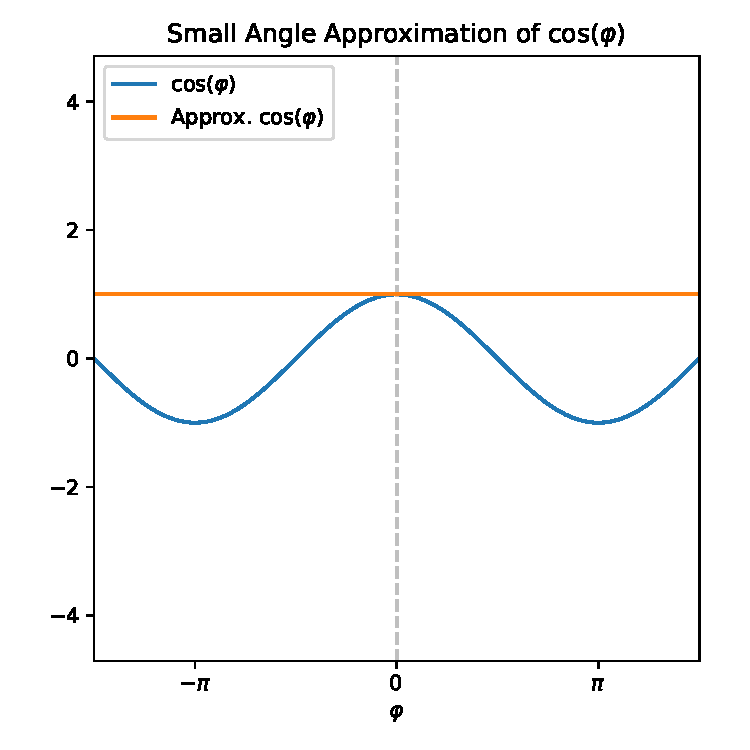
\includegraphics[width = \linewidth]{figures/introduction/generated/small-angle-approximation-cos.pdf}
			\caption{Small angle approximation \( \cos(\varphi) \approx 1 \) of Cosine.}
		\end{subfigure}
		\caption{Visualization of the small angle approximation (given in orange) of the basic trigonometric functions Sine and Cosine (given in blue). It is clear that the approximation is only valid in a small region around zero (\( \varphi \approx 0 \)).}
		\label{fig:smallAngleApproximation}
	\end{figure}

	We now look at two examples of dynamical systems, one of which is linear and one that is not.

	\paragraph{Harmonic Oscillator}
		\label{subsec:harmonicOscillator}

		\begin{figure}
			\centering
			\tikzHarmonicOscillator
			\caption{Illustration of a simple harmonic oscillator with mass \(m\), spring stiffness \(k\) and position \(x\) that is not affected by any external force like gravity. The mass is in equilibrium if \( x = 0 \).}
			\label{fig:simpleHarmonicOscillator}
		\end{figure}

		The \emph{simple harmonic oscillator} describes the dynamical system of a mass \(m\) that is attached to a spring that is following Hooke's Law with stiffness \(k\) (see~\autoref{fig:simpleHarmonicOscillator}). This harmonic oscillator is described by the \ac{ode}
		\begin{equation}
			m\ddot{x} = -kx \quad\iff\quad \ddot{x} = -\frac{k}{m} x  \label{eq:harmonicOscillator}
		\end{equation}
		where \(x\) and \(\ddot{x}\) are the position and acceleration of the mass, respectively. Note that if \( x = 0 \), the mass is in equilibrium and no force is acting on it.

		By using basic results in the solution theory of linear \acp{ode}, we see that the general solution is given as
		\begin{equation*}
			x(t) = A \cos\Big(t \sqrt{k / m} + \varphi\Big)
		\end{equation*}
		with the amplitude \(A\) and the phase \(\varphi\) (see~\autoref{app:harmonicOscillatorSolution} for the derivation of the solution). As neither gravity nor damping or other external forces are involved in the dynamical system, the motion continues forever with a non-changing amplitude.
	% end

	\paragraph{Simple Pendulum}
		\label{subsec:simplePendulum}

		\begin{figure}
			\centering
			\tikzSimplePendulum
			\caption{Illustration of an inverse pendulum with mass \(m\) and displacement \(\varphi\) that is only affected by gravity and no other external force. The mass is in equilibrium for both \( \varphi = 0 \) and \( \varphi = \pi \), where the former is an unstable equilibrium.}
			\label{fig:simplePendulum}
		\end{figure}

		The \emph{inverse pendulum} describes the dynamical system of a mass \(m\) that is attached to a rigid pole of length \(L\) which can freely swing around a suspension point (see~\autoref{fig:simplePendulum}). The pendulum stands upright if \( \varphi = 0 \) and its equation of motion is described by the \ac{ode}
		\begin{equation*}
			\ddot{\varphi} = \frac{g}{L} \sin(\varphi)
		\end{equation*}
		where \(g\), \(L\), \(\varphi\) and \(\ddot{\varphi}\) describe the gravity acceleration, pole length, displacement and acceleration of the mass, respectively. Note that if \( \varphi = 0 \), the mass is in an unstable equilibrium and no force is acting on it.

		In comparison to the harmonic oscillator (\autoref{subsec:harmonicOscillator}), this differential equation is nonlinear. And, even for the case with unit gravity acceleration \( g = 1 \) and unit pole length \( L = 1\), where the \ac{ode} looks really simple
		\begin{equation}
			\ddot{\varphi} = \sin(\varphi)  \label{eq:inversePendulum}
		\end{equation}
		it is not tractable analytically (\ac{ie} there exists no solution in closed form).

		Still, we can apply the small angle approximation introduced before (in this case, \( \sin(\varphi) \approx \varphi \)) which yields the simple \ac{ode}
		\begin{equation}
			\ddot{\varphi} \approx \varphi  \label{eq:linearizedInversePendulum}
		\end{equation}
		solved by
		\begin{equation*}
			\varphi(t) = \frac{1}{2} e^{-t} \big(\varphi_0 + e^{2t} \varphi_0 - \dot{\varphi}_0 + e^{2t} \dot{\varphi}_0\big)
		\end{equation*}
		where \(\varphi_0\) and \(\dot{\varphi}_0\) are the initial displacement and velocity, respectively.

		However, this small angle approximation can only forecast small displacements \( \varphi \ll \pi/2 \). And, as the equilibrium at \( \varphi = 0 \) is unstable, the approximation becomes worse as time goes by because the pendulum falls down. This behavior is shown in~\autoref{fig:inversePendulumApprox}.

		\begin{figure}
			\centering
			\begin{subfigure}[t]{0.5\linewidth}
				\centering
				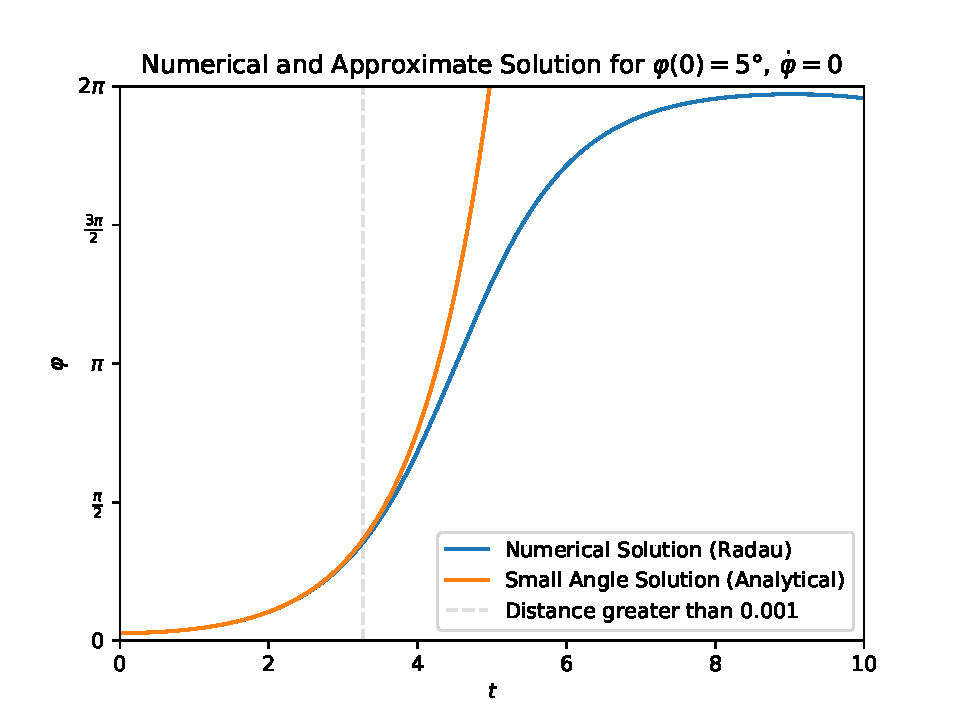
\includegraphics[width = \linewidth]{figures/introduction/generated/pendulum-motion-solutions}
				\caption{Trajectories of two solution strategies to the inverse pendulum, where the blue is a numerical solution of the actual motion of equation (solved using the Radau~IIA method~\cite[p.~72]{guglielmiImplementingRadauIIA2001}) and the orange one is the analytically computed solution linearized \ac{ode}. The latter is linearized using small angle approximation. The dashed gray vertical line shows when the distance tolerance of \( \varepsilon = 10^{-3} \) is exceeded.}
			\end{subfigure}%
			~
			\begin{subfigure}[t]{0.5\linewidth}
				\centering
				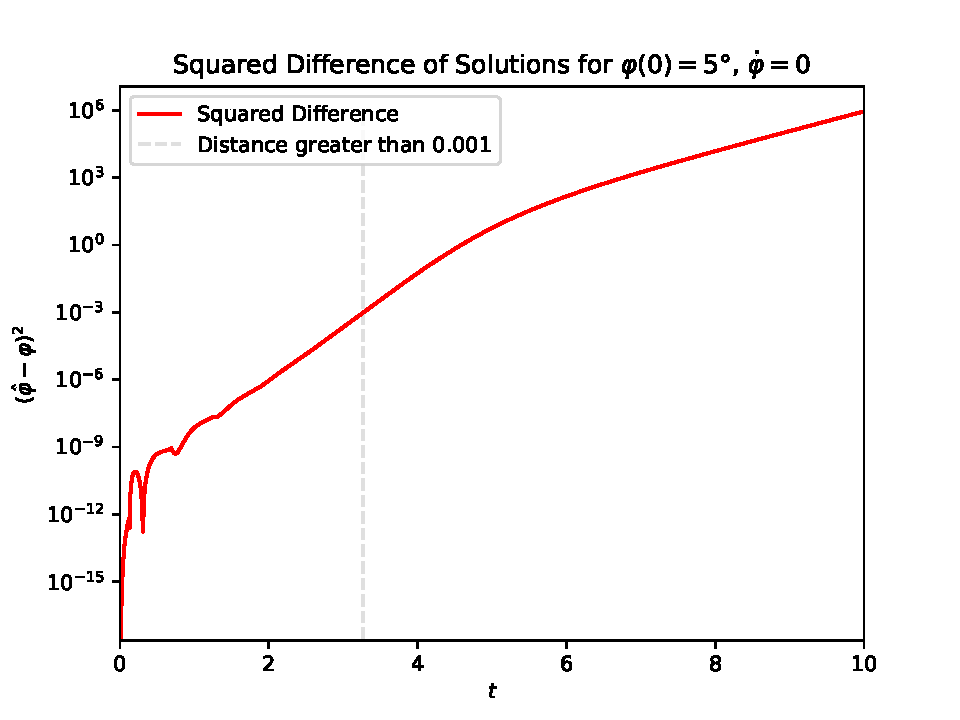
\includegraphics[width = \linewidth]{figures/introduction/generated/pendulum-motion-difference}
				\caption{Differences between the small angle approximation and the numerical solution of the \ac{ode}. The dashed gray vertical line shows when the distance tolerance of \( \varepsilon = 10^{-3} \) is exceeded.}
			\end{subfigure}
			\caption{Comparison of a numerical solution to the \ac{ode} of the inverse pendulum given in~\eqref{eq:inversePendulum} and the analytical solution of the linearized \ac{ode} given in~\eqref{eq:linearizedInversePendulum}. A tolerance value of \( \varepsilon = 10^{-3} \) is used to show when both solutions diverge from each other.}
			\label{fig:inversePendulumApprox}
		\end{figure}
	% end

	\subsection{Discrete-Time Dynamical Systems}
		In comparison to continuous-time dynamical systems described by \acp{ode}, discrete-time systems are described by a \emph{dynamics function} \( \vec{F} : \R^n \to \R^n \) advancing all states forward in time:
		\begin{equation*}
			\vec{x}_{t + 1} = \vec{F}(\vec{x}_t)
		\end{equation*}
		But we should note that, while seeming more restrictive, discrete-time dynamical systems are more general than continuous-time systems as we can discretize every continuous-time system
		\begin{equation*}
			\dot{\vec{x}} = \vec{f}(\vec{x})
		\end{equation*}
		as a discrete-time dynamical system
		\begin{equation*}
			\vec{x}_{t + 1} = \vec{F}(\vec{x}_t)
		\end{equation*}
		using the state dynamics function
		\begin{equation*}
			\vec{F}\big(\vec{x}(t_0)\big) = \vec{x}(t_0 + \Delta_t) = \vec{x}(t_0) + \int_{t_0}^{t_0 + \Delta_t} \! \vec{f}\big(\vec{x}(\tau)\big) \dd{\tau}
		\end{equation*}
		where \( \Delta_t \) is called the \emph{discretization interval} and \( \vec{x}_k = \vec{x}(k \Delta_t) \). From the Nyquist-Shannon sampling theorem, we know for band-limited functions that the sampling rate \( f_s = 1/\Delta_t \) has to be greater than two times the maximum frequency of the original function~\cite{shannonCommunicationPresenceNoise1949}, \ac{ie} \( f_s = 1/\Delta_t > 2 f \).
	% end
% end

	\chapter{Related Work}
	\label{c:relatedWork}

	% See references mindmap.

	\todo{Related Work}
% end

	\chapter{Koopman Theory of Dynamical Systems}
\label{c:koopmanTheoryOfDynamicalSystems}



In the previous chapter we have seen that we are in the need of a linearization technique that generalizes globally, not only locally like the small angle approximation. This brings us directly to Koopman theory, original introduced by Bernard Koopman in 1931~\cite{koopmanHamiltonianSystemsTransformation1931} in the context of Hamiltonian systems and transformations in Hilbert spaces. Considering a nonlinear discrete-time dynamical system
\begin{align*}
	\vec{s}_{t + 1} = \vec{F}(\vec{s}_t),\quad \vec{F} : \R^k \to \R^k
\end{align*}
and observations \( \vec{g} : \R^p \to \R^p \) of this system, \ac{ie} \( \vec{g}_t \coloneqq \vec{g}(\vec{s}_t) \), the infinite-dimensional \emph{Koopman operator} \(\mathcal{K}\) advances all of the measurements forward in time. This relation can also be expressed as the composition
\begin{align*}
	\mathcal{K} \vec{g} \coloneqq \vec{g} \circ \vec{F} \qquad\iff\qquad \mathcal{K} \vec{g}(\vec{s}_t) = \vec{g}\big( \vec{F}(\vec{s}_t) \big) = \vec{g}(\vec{s}_{t + 1})
\end{align*}
This relation is true for every possible measurement function \( \vec{g} \) at any point of the system space \( \R^k \)~\cite{bruntonKoopmanInvariantSubspaces2016}. All possible measurement functions \( \vec{g} \) span an infinite-dimensional Hilbert space \( \mathcal{G} \). A finite set of measurements \( \vec{g}_1, \vec{g}_2, \cdots, \vec{g}_p \) that span an invariant subspace \( \mathcal{G}' \subset \mathcal{G} \), \ac{ie} applying the Koopman operator to a linear combination of these functions keeps them in the subspace
\begin{align*}
	\vec{g} &= \alpha_1 \vec{g}_1 + \alpha_2 \vec{g}_2 + \cdots + \alpha_p \vec{g}_p \\
	\mathcal{K} \vec{g} &= \beta_1 \vec{g}_1 + \beta_2 \vec{g}_2 + \cdots + \beta_p \vec{g}_p
\end{align*}
can be considered as a basis of that subspace. If that is possible, we can restrict the Koopman operator onto \( \mathcal{G}' \). Functions that both span the subspace \(\mathcal{G}'\) and do only scale when applying the Koopman operator, \ac{ie} \( \mathcal{K} \vec{\varphi} = \lambda \vec{\varphi} \) are called \emph{Eigenfunctions} of the Koopman operator. Finding these Eigenfunctions is extremely desirable, as it allows us to get a finite Koopman operator \( \mat{K} \) globally linearizing the dynamical system \( \vec{F} \).

For this thesis, we do not focus on finding the actual Eigenfunctions but to just approximate them.

	\chapter{Inference in Dynamical Systems}
\label{c:inferenceInDynamicalSystems}



\todo{Inference in Dynamical Systems}

\section{Hidden Markov Models and LGDS}
	% HMM with cintinuous state --> LGDS

	\todo{Inference: HMM and LGDS}
% end

\section{Filtering and Smoothing}
	\subsection{Filtering and Smoothing}

	\subsection{Kalman Filter}
		\todo{Filtering: Kalman}
	% end

	\subsection{Rauch-Tung-Striebel/Kalman Smoother}
		\todo{Filtering: RTS}
	% end
% end

\section{Cubature Rules and Filtering}
	\todo{Inference: Cubature}

	\subsection{Square-Root Filtering/Smoothing}
		\todo{Cubature: Sqrt Filtering}
	% end
% end

	\chapter{The Nonlinear Gaussian Koopman Algorithm}  % TODO: Find better name.
\label{c:nonlinearGaussianKoopman}
\IMRADlabel{methods}



In this chapter we will introduce out contribution and the theoretical background of the \algname algorithm that we will implement as a proof of concept in~\autoref{c:experiments}. We will start by introducing the ideas that lead to the idea, then formulate and also solve the arising (approximate) inference problem.

By looking at the graphical model for an \ac{lgds} and the state transition model for a Koopman dynamical system in~\autoref{fig:lgdsKoopmanRelation}, we can see that there are lots of similarities. The first and most interesting similarity is that both systems assume a latent state that transitions linearly, either with a state dynamics matrix \(\mat{A}\) for the \ac{lgds} or with the Koopman operator\footnote{From now on, we assume a finite-dimensional matrix approximation \(\mat{K}\) of the Koopman operator \(\mathcal{K}\).} \(\mat{K}\). The greatest difference is that measurements in classic \ac{lgds} are taken linearly with an observation matrix \( \mat{C} \) and nonlinear in the Koopman system with the measurement function \( \vec{h}(\cdot) \).

\begin{figure}
	\centering
	\begin{subfigure}[t]{0.5\linewidth}
		\centering
		\resizebox{\linewidth}{!}{\tikzLinearGaussianDynamicalSystem}
		\caption{Graphical model of a linear Gaussian dynamical system with the latent state \(\vec{s}_t\) and the (linear) observations \(\vec{y}_t\). In contrast to the Koopman system, this system is not deterministic and the arrows represent probabilistic dependency rather than hard transitions.}
	\end{subfigure}%
	\begin{subfigure}[t]{0.5\linewidth}
		\centering
		\resizebox{\linewidth}{!}{\tikzKoopmanOperator}
		\caption{State transition model of a Koopman dynamical system with the Koopman operator \( \mathcal{K} \) that can be approximated with a matrix \(\mat{K}\). In contrast to the \ac{lgds}, the state is represented via nonlinear transitions and the observations are the linear dynamics. \\ Adopted from~\cite{bruntonKoopmanInvariantSubspaces2016}.}
	\end{subfigure}
	\caption{Side-by-side comparison of the a \ac{lgds} on the left and a Koopman dynamical system on the right. This side-by-side view highlights our idea of interpreting an Koopman system as a semi-linear dynamical system (\ac{ie} an \ac{lgds} with nonlinear observations).}
	\label{fig:lgdsKoopmanRelation}
\end{figure}

Our idea is to "flip" the Koopman dynamical system and replace the observation matrix \( \mat{C} \) with a nonlinear observation function \( \vec{g}(\cdot) \), that takes the linear states \( \vec{s}_t \) and maps them into a nonlinear observation space \( \vec{y}_t \). In other words, we seek to find the inverse function of \( \vec{h}(\cdot) \) to map out of the linear embedding that Koopman theory guarantees us to exist. Our belief that such an inverse function exists is backed by previous accomplishments in data-driven Koopman analysis~\cite{luschDeepLearningUniversal2018} that also seek and find such an inverse mapping (see~\ref{c:relatedWork} for more information).

Additionally, we contribute a probabilistic view on the Koopman operator, being able to gauche our uncertainty about the embedding and the inverse mapping to the observation space. Speaking of the observation space, this is a good point to clear up chaos of notation and names that builds up when working with two systems where "observation" means contrary concepts. From now on, we will work on the graphical system shown in~\autoref{fig:nonlinearGaussianKoopman} characterized by the dynamics
\begin{align*}
	\vec{s}_{t + 1} &= \eqmakebox[ngkIntro][l]{\( \mat{A} \vec{s}_t + \vec{w}_t,\quad \vec{w}_t \)} \sim \normal(\vec{0}, \mat{Q}) \\
	\vec{y}_t       &= \eqmakebox[ngkIntro][l]{\( \vec{g}(\vec{s}_t) + \vec{v}_t,\quad \vec{v}_t \)} \sim \normal(\vec{0}, \mat{R})
\end{align*}
that can equivalently be formulated as
\begin{align*}
	\vec{s}_{t + 1} &\sim \normal(\mat{A} \vec{s}_t, \mat{Q}) \\
	\vec{y}_t       &\sim \normal\big(\vec{g}(\vec{s}_t), \mat{R}\big)
\end{align*}
We call \( \vec{s}_t \) the \emph{latent variables} or \emph{latents} in the \emph{latent space} with dimensionality \(k\), \( \vec{y}_t \) the \emph{observation variables} or \emph{observations} in the \emph{observation space} with dimensionality \(p\), \( \vec{g} : \R^k \to \R^p \) the \emph{observation function} mapping latents to observations, \( \mat{A} \) the \emph{(state) dynamics matrix}, \( \mat{Q} \) the state covariance matrix and \( \mat{R} \) the observation covariance matrix.

\begin{figure}
	\centering
	\tikzNonlinearGaussianKoopman
	\caption{The graphical model of the \algname model. Given an observation sequence \( \vec{y}_{1:T} \), we seek the latent dynamics and the corresponding nonlinear mapping \( \vec{g}(\cdot) \) from the latent space to the observations.}
	\label{fig:nonlinearGaussianKoopman}
\end{figure}

%\section{Formulating and Solving the Nonlinear Approximate Inference Problem using an Approximate EM Algorithm}
\section{Formulating and Solving the Inference Problem using an EM Algorithm}
	% Formulate likelihood, expected likelihood.
	% Shortly outline how to do the derivation and reference appendix.
	% Summarize M-step equations.
	% Combine ideas from ch. 2 (cubature and sqrt) and summarize.

	%Instead of tackling the inference problem with some kind of \ac{vae}, we choose to use an \ac{em} algorithm as it requires less training because of putting more prior knowledge and assumptions into the model, like the Gaussian noise or the specific

	We seek to find the matrices \(\mat{A}\), \(\mat{Q}\) and \(\mat{R}\) and the observation function \( \vec{g}_{\vec{\theta}}(\cdot) \), parameterized by \(\vec{\theta}\) and the initial state distribution \( \vec{s}_1 \sim \normal(\vec{m}_0, \mat{V}_0) \) that maximize the likelihood
	\begin{equation*}
		p(\vec{s}_{1:T}, \vec{y}_{1:T}) = p(\vec{s}_1) \prod_{t = 2}^{T} p(\vec{s}_t \given \vec{s}_{t - 1}) \prod_{t = 1}^{T} p(\vec{y}_t \given \vec{s}_t)
	\end{equation*}
	which factors over the conditional distributions due to the Markovian assumption. For brevity, we will keep the parameters \( \vec{\theta} \) of the observation function \( \vec{g}_{\vec{\theta}}(\cdot) \) implicit from now on. Subsequently, we can proceed by not maximizing the likelihood but the log-likelihood which is easier to maximize as the Gaussian lies in the exponential family, exhibiting a convex optimization problem\footnote{Strictly speaking, the optimization problem is only convex \ac{wrt} \(\mat{A}\) and \(\mat{Q}\). For \(\mat{R}\) and \(\vec{\theta}\), the problem is still non-convex, but numerically more stable as sums is easier to differentiate and to compute than products.}:
	\begin{equation*}
		\log p(\vec{s}_{1:T}, \vec{y}_{1:T}) = \log p(\vec{s}_1) + \sum_{t = 2}^{T} \log p(\vec{s}_t \given \vec{s}_{t - 1}) + \sum_{t = 1}^{T} \log p(\vec{y}_t \given \vec{s}_t)
	\end{equation*}
	Inserting the Gaussian distributions
	\begin{equation*}
		p(\vec{s}_1) = \normal(\vec{s}_1 \given \vec{m}_0, \mat{V}_0) \qquad\qquad
		p(\vec{s}_t \given \vec{s}_{t - 1}) = \normal(\vec{s}_t \given \mat{A} \vec{s}_{t - 1}, \mat{Q}) \qquad\qquad
		p(\vec{y}_t \given \vec{s}_t) = \normal\big(\vec{y}_t \given \vec{g}(\vec{s}_t), \mat{R}\big)
	\end{equation*}
	yields the log-likelihood
	\begin{align*}
		\log p(\vec{s}_{1:T}, \vec{y}_{1:T})
			&= -\frac{T(k + p)}{2} \log(2\pi) - \frac{1}{2} \log \lvert \mat{V}_0 \rvert - \frac{T - 1}{2} \log \lvert \mat{Q} \rvert - \frac{T}{2} \log \lvert \mat{R} \rvert \\
			&\qquad\qquad -\frac{1}{2} (\vec{s}_1 - \vec{m}_0)^T \mat{V}_0^{-1} (\vec{s}_1 - \vec{m}_0) \\
			&\qquad\qquad -\frac{1}{2} \sum_{t = 2}^{T} (\vec{s}_t - \mat{A} \vec{s}_{t - 1})^T \mat{Q}^{-1} (\vec{s}_t - \mat{A} \vec{s}_{t - 1}) \\
			&\qquad\qquad -\frac{1}{2} \sum_{t = 1}^{T} (\vec{y}_t - \vec{g}_t)^T \mat{R}^{-1} (\vec{y}_t - \vec{g}_t)
	\end{align*}
	with the abbreviation \( \vec{g}_t \coloneqq \vec{g}(\vec{s}_t) \).

	But maximizing this quantity is impossible as we do not have the latent states \( \vec{s}_{1:T} \). Hence, as usual in \ac{em} \todo{see section xy}, we instead maximize the expected log-likelihood and estimate the latent states based on out previous guess for the state dynamics. These two steps form our E- and M-step of the \algname algorithm:
	\begin{itemize}
		\item E-Step: Estimate the latent states \( \vec{s}_{1:T} \).
		\item M-Step: Maximize the expected log-likelihood \ac{wrt} the state dynamics and observation function parameters.
	\end{itemize}
	We will proceed with deriving the M-step and finish this section off by deriving the E-step. Please be aware that we only briefly touch the derivation here and focus on the important steps. See~\autoref{app:fullNgkDerivation} for the complete derivation with explanations throughout every step.

	For the M-step, we first need the expected log-likelihood \( Q \coloneqq \E_{\vec{s}_{1:T}}\big[ p(\vec{s}_{1:T}, \vec{y}_{1:T}) \big] \) as stated previously. This quantity depends on three expectations that be estimate in the E-step:
	\begin{align*}
		\hat{\vec{s}}_{t \subgiven t_0}^{(n)}  & \coloneqq \E\Big[\vec{s}_t^{(n)} \Biggiven \vec{y}_{1:t_0}\Big]                             & \hat{\vec{s}}_{t \subgiven t_0}           & \coloneqq \frac{1}{N} \sum_{n = 1}^{N} \hat{\vec{s}}_{t \subgiven t_0}^{(n)}  \\
		\mat{P}_{t \subgiven t_0}^{(n)}        & \coloneqq \E\Big[\vec{s}_t^{(n)} \vec{s}_t^{(n), T} \bigggiven \vec{y}_{1:t_0}\Big]       & \mat{P}_{t \subgiven t_0}        & \coloneqq \frac{1}{N} \sum_{n = 1}^{N} \mat{P}_{t \subgiven t_0}^{(n)}        \\
		\mat{P}_{t, t - 1 \subgiven t_0}^{(n)} & \coloneqq \E\Big[\vec{s}_t^{(n)} \vec{s}_{t - 1}^{(n), T} \bigggiven \vec{y}_{1:t_0}\Big] & \mat{P}_{t, t - 1 \subgiven t_0} & \coloneqq \frac{1}{N} \sum_{n = 1}^{N} \mat{P}_{t, t - 1 \subgiven t_0}^{(n)}
	\end{align*}
	These expectations are called the expected state, the self-correlation and the cross-correlation, respectively. We also silently introduced an upper index, \( \cdot^{(n)} \), which indicated which observation sequence our observation is from, because the algorithm can simultaneously learn on \(N\) observation sequences. For brevity, we may write \( \hat{\vec{s}}_t \) instead of \( \hat{\vec{s}}_{t \subgiven T} \) (analogous for all other values). Additionally, we have to define two quantities for the expectations of the nonlinear observation function \( \vec{g} \) that we cannot evaluate in closed form:
	\begin{align*}
		\hat{\vec{g}}_t^{(n)} &\coloneqq \E\Big[\vec{g}_t^{(n)} \Biggiven \vec{y}_{1:T}\Big] \\
		\mat{G}_t^{(n)}       &\coloneqq \E\Big[\vec{g}_t^{(n)} \vec{g}_t^{(n), T} \Biggiven \vec{y}_{1:T}\Big]
	\end{align*}
	We can now evaluate the expected log-likelihood depending on the above quantities using the trace-trick\footnote{The trace of a product of matrices/vectors is invariant under even permutations of the matrices/vectors within the trace.}, giving the following (enormous) quantity:
	\begin{align*}
		Q
			&= \E_{\vec{s}_{1:T}}\big[ p(\vec{s}_{1:T}, \vec{y}_{1:T}) \big] \\
			&= -\frac{NT(k + p)}{2} \ln(2\pi) - \frac{N}{2} \ln \lvert \mat{V}_0 \rvert - \frac{N(T - 1)}{2} \ln \lvert \mat{Q} \rvert - \frac{NT}{2} \ln \lvert \mat{R} \rvert \\
			&\qquad\qquad -\frac{N}{2} \tr\!\Big( \mat{P}_1 \mat{V}_0^{-1} \Big) + \frac{N}{2} \tr\!\Big( \hat{\vec{s}}_1 \vec{m}_0^T \mat{V}_0^{-1} \Big) + \frac{N}{2} \tr\!\Big( \vec{m}_0 \hat{\vec{s}}_1^T \mat{V}_0^{-1} \Big) - \frac{N}{2} \tr\!\Big(\vec{m}_0 \vec{m}_0^T \mat{V}_0^{-1} \Big) \\
			&\qquad\qquad -\frac{N}{2} \sum_{t = 2}^{T} \tr\!\Big( \mat{P}_t \mat{Q}^{-1} \Big) - \tr\!\Big( \mat{P}_{t, t - 1} \mat{A}^T \mat{Q}^{-1} \Big) - \tr\!\Big( \mat{A} \mat{P}_{t, t - 1} \mat{Q}^{-1} \Big) - \tr\!\Big( \mat{A} \mat{P}_{t - 1} \mat{A}^T \mat{Q}^{-1} \Big) \\
			&\qquad\qquad -\frac{1}{2} \sum_{n = 1}^{N} \sum_{t = 1}^{T} \tr\!\Big( \vec{y}_t^{(n)} \vec{y}_t^{(n), T} \mat{R}^{-1} \Big) - \tr\!\Big( \vec{y}_t^{(n)} \hat{\vec{g}}_t^{(n), T} \mat{R}^{-1} \Big) - \tr\!\Big( \hat{\vec{g}}_t^{(n)} \vec{y}_t^{(n), T} \mat{R}^{-1} \Big) + \tr\!\Big( \mat{G}_t^{(n)} \mat{R}^{-1} \Big)
	\end{align*}
	By maximizing this quantity \ac{wrt} the dynamics matrix \(\mat{A}\), the covariance matrices \(\mat{Q}\) and \(\mat{R}\), the initial state mean \(\vec{m}_0\) and the initial state covariance \(\mat{V}_0\), \ac{ie} setting the derivative \ac{wrt} these parameters to zero and rearranging the equations, we get the closed-form solutions
	\begin{align*}
		\mat{A}^\new   &= \Bigg(\! \sum_{t = 2}^{T} \mat{P}_{t, t - 1} \!\Bigg) \Bigg(\! \sum_{t = 2}^{T} \mat{P}_{t - 1} \!\Bigg)^{-1} \\
		\mat{Q}^\new   &= \frac{1}{T - 1} \Bigg(\! \sum_{t = 2}^{T} \mat{P}_t - \mat{A}^\new \sum_{t = 2}^{T} \mat{P}_{t, t - 1} \!\Bigg) \\
		\vec{m}_0^\new &= \hat{\vec{s}}_1 = \frac{1}{N} \sum_{n = 1}^{N} \hat{\vec{s}}_1^{(n)} \\
		\mat{V}_0^\new &= \mat{P}_1 - \hat{\vec{s}}_1 \hat{\vec{s}}_1^T \\
		\mat{R}^\new   &= \frac{1}{NT} \sum_{n = 1}^{N} \sum_{t = 1}^{T} \vec{y}_t^{(n)} \vec{y}_t^{(n), T} - \hat{\vec{g}}_t^{(n)} \vec{y}_t^{(n), T} - \vec{y}_t^{(n)} \hat{\vec{g}}_t^{(n), T} + \mat{G}_t^{(n), T}
	\end{align*}
	where we assume an optimal \( \vec{g}(\cdot) \) for the last equation for \(\mat{R}\). To maximize the expected log-likelihood \ac{wrt} the observation function \( \vec{g} \), we choose a learnable function approximator, \ac{eg} a neural network and maximize \(Q\) using simple gradient descent or a more evolved optimizer like Adam~\cite{kingmaAdamMethodStochastic2017}. We should note that we do not need to fully maximize \(Q\) in every M-step but that it is enough to just get better in every M-step for the convergence properties to still hold~\cite{dempsterMaximumLikelihoodIncomplete1977a}.

	We now turn to the problem of evaluating \( \hat{\vec{g}}_t^{(n)} \) and \( \mat{G}_t^{(n)} \). Instead of using Monte Carlo methods that are both very computationally expensive (especially as the gradient has to flow through the evaluation), we are employing the spherical-radial cubature rule that we have introduced in~\autoref{sec:cubatureRules}. That way, we can approximate the integrals both efficient and deterministically (as compared to Monte Carlo methods):
	\begin{align}
		\hat{\vec{g}}_t^{(n)} &= \int\! \vec{g}_t^{(n)} p\Big(\vec{s}_t^{(n)} \Biggiven \vec{y}_{1:T}\Big) \dd{\vec{s}_{1:T}^{(n)}} \approx \SRC\Big[\vec{g};\, \hat{\vec{s}}_t^{(n)}, \mat{V}_t^{(n)}\Big]  \label{eq:ngkgeval} \\
		\mat{G}_t^{(n)}       &= \int\! \vec{g}_t^{(n)} \vec{g}\vec{s}_t^{(n), T} p\Big(\vec{s}_t^{(n)} \Biggiven \vec{y}_{1:T} \Big) \dd{\vec{s}_{1:T}^{(n)}} \approx \SRC\Big[\vec{g} \vec{g}^T;\, \hat{\vec{s}}_t^{(n)}, \mat{V}_t^{(n)}\Big]  \label{eq:ngkGeval}
	\end{align}
	This concludes the derivation of the M-step, where we do not have explicit formulas for the observation parameters \(\vec{\theta}\) as we do learn these using a numerical optimizer.

	Deriving the E-step is quite straightforward given the groundwork we developed in~\autoref{sec:filteringSmoothing} and~\autoref{subsec:cubatureFiltering}. As we heavily employ cubature rules in the M-step (in fact, in every \ac{gd} iteration in the M-step), we chose to use a square-root Kalman filter and a square-root \ac{rts} smoother to directly get the Cholesky decomposition of the used covariance matrices. We apply~\autoref{alg:sqrtCubatureKalmanFilter} after afterwards~\autoref{alg:sqrtCubatureRtsSmoother} with the state dynamics function \( \vec{f} : \R^k \to \R^k : \vec{s} \mapsto \mat{A} \vec{s} \) and the observations function \( \vec{g}_{\vec{\theta}} \). Additionally to the covariances, we have to compute the self- and cross-correlation. Following~\cite{minkaHiddenMarkovModels1999}, they are given as
	\begin{align*}
		\mat{P}_t^{(n)} &= \hat{\mat{V}}_t^{(n)} - \hat{\vec{s}}_t^{(n)} \hat{\vec{s}}_t^{(n), T} \\
		\mat{P}_{t, t - 1}^{(n)} &= \hat{\mat{J}}_{t - 1} \hat{\mat{V}}_t - \hat{\vec{s}}_{t}^{(n)} \hat{\vec{s}}_{t - 1}^{(n), T}
	\end{align*}

	The whole \algname algorithm is outline in~\autoref{alg:ngk}.

	\begin{algorithm}  \DontPrintSemicolon
		\KwData{\(N\) observation sequences \( \vec{y}_{1:T}^{(n)} \in \R^{p \times T} \).}
		\textbf{Initialize} \(\mat{A}\), \(\mat{Q}\), \(\mat{R}\), \(\vec{m}_0\), \(\mat{V}_0\) and \(\vec{\theta}\) somehow (\ac{eg} identity matrices). \;
		\While{not converged}{
			\tcp{\textbf{E-Step:}}
			\( \displaystyle \vec{s}_{1:T}^{(1:N)},\, \hat{\mat{V}}_{1:T} \gets \text{\ac{rts}-Smoother} \) \;
			\eqmakebox[ngkestep][r]{\( \displaystyle \mat{P}_t^{(n)} \gets \)} \( \displaystyle \hat{\mat{V}}_t^{(n)} - \hat{\vec{s}}_t^{(n)} \hat{\vec{s}}_t^{(n), T} \) for \( t = 1, 2, \rangedots, T \) and \( n = 1, 2, \rangedots, N \) \;
			\eqmakebox[ngkestep][r]{\( \displaystyle \mat{P}_{t, t - 1}^{(n)} \gets \)} \( \displaystyle \hat{\mat{J}}_{t - 1} \hat{\mat{V}}_t - \hat{\vec{s}}_{t}^{(n)} \hat{\vec{s}}_{t - 1}^{(n), T} \) for \( t = 2, 3, \rangedots, T \) and \( n = 1, 2, \rangedots, N \) \;
			\tcp{\textbf{M-Step:}}
			\eqmakebox[ngkmstep][r]{\( \displaystyle \vec{\theta} \gets \)} \( \text{\ac{gd}}\big(Q(\vec{\theta})\big) \) \;
			\eqmakebox[ngkmstep][r]{\( \displaystyle \mat{R} \gets \)} \( \displaystyle \frac{1}{NT} \sum_{n = 1}^{N} \sum_{t = 1}^{T} \vec{y}_t^{(n)} \vec{y}_t^{(n), T} - \hat{\vec{g}}_t^{(n)} \vec{y}_t^{(n), T} - \vec{y}_t^{(n)} \hat{\vec{g}}_t^{(n), T} + \mat{G}_t^{(n), T} \) \;
			\eqmakebox[ngkmstep][r]{\( \displaystyle \mat{A} \gets \)} \( \displaystyle \Bigg(\! \sum_{t = 2}^{T} \mat{P}_{t, t - 1} \!\Bigg) \Bigg(\! \sum_{t = 2}^{T} \mat{P}_{t - 1} \!\Bigg)^{-1} \) \;
			\eqmakebox[ngkmstep][r]{\( \displaystyle \mat{Q} \gets \)} \( \displaystyle \frac{1}{T - 1} \Bigg(\! \sum_{t = 2}^{T} \mat{P}_t - \mat{A}^\new \sum_{t = 2}^{T} \mat{P}_{t, t - 1} \!\Bigg) \) \;
			\eqmakebox[ngkmstep][r]{\( \displaystyle \vec{m}_0 \gets \)} \( \displaystyle \frac{1}{N} \sum_{n = 1}^{N} \hat{\vec{s}}_1^{(n)} \) \;
			\eqmakebox[ngkmstep][r]{\( \displaystyle \mat{V}_0 \gets \)} \( \displaystyle \mat{P}_1 - \hat{\vec{s}}_1 \hat{\vec{s}}_1^T \) \;
		}
		\caption{\algname}
		\label{alg:ngk}
	\end{algorithm}
% end

\section{Implementation}
	\label{sec:implementation}

	We implemented the \algname algorithm in Python using the popular array processing library NumPy~\cite{harrisArrayProgrammingNumPy2020} throughout the whole implementation, the deep learning library PyTorch~\cite{paszkePyTorchImperativeStyle2019} for the numerical optimization of \(\vec{\theta}\) and Sacred~\cite{greffSacredInfrastructureComputational2017} for experiment management. The whole implementation can be found on GitHub\footnote{See \href{https://github.com/fdamken/bachelors-thesis_code}{\texttt{https://github.com/fdamken/bachelors-thesis\_code}}.}.

	During the implementation we focused on making the algorithm as reusable as possible, separating all data generation and investigation code from the actual implementation. Separating the data generation also has the advantage that we can run benchmarks on the exact same data to compare model performance. We have separated the optimization of \(\vec{\theta}\) as much as possible (as outlined in~\autoref{alg:ngk}) and made it possible for the user of the algorithm to easily change the optimization algorithm to use in conjunction with the parameters of the algorithm like the learning rate (defaulting to Adam~\cite{kingmaAdamMethodStochastic2017} with a learning rate of \( 0.01 \)). We also made all of the following configurable:
	\begin{itemize}
		\item Whether to perform whitening of the observation data or not. That is, if we perform whitening, we normalize and standardize the training observations beforehand using \( \hat{\vec{y}}_{1:T, i} = (\vec{y}_{1:T, i} - \bar{\vec{y}}_i) / \sigma_{y_i} \) where \( \bar{\vec{y}}_i \) is the mean and \( \sigma_{y_i} \) is the standard deviation of the \(i\)-th component of all measurements. Doing the whitening first sometimes improves the performance as we will see in~\ref{c:experiments}.
		\item The convergence precision, \ac{ie} how much the log-likelihood has to change in order to continue the \ac{em} iterations. We will see that, due to numerical instabilities and approximation errors in the cubature rules, the algorithm rarely really converges before becoming numerically unstable.
		\item That is why we also made the maximum number of iterations configurable to support \emph{early stopping}. Once the algorithm performed these number of \ac{em} iterations, it will abort and report the results.
		\item Similarly it is possible to configure the convergence precision and maximum number of iterations for the subsequent optimization of \(\vec{\theta}\).
	\end{itemize}
	These are only the parameters that can be configured directly on the \ac{em} algorithm, but the user is also able to specify how to initialize everything, \ac{ie} the matrices \( \mat{A} \), \( \mat{Q} \), \( \mat{R} \), \( \mat{V}_0 \), \( \vec{m}_0 \) and the parameters \( \vec{\theta} \) of the observation function \( \vec{g}_{\vec{\theta}} \). Speaking of the observation function, we used a neural network with \( \tanh \) activation function and a single hidden layer for all experiments (see~\autoref{c:experiments} for more information about the experiment setup). We made it also possible to pass arbitrary Torch modules as the function approximator that can be learned via a \ac{gd}-like algorithm (\ac{ie} they must be differentiable and expose parameters).

	For learning multiple observation sequences, as outlined in the derivation of the \algname algorithm in~\autoref{c:nonlinearGaussianKoopman}, it turns out to be useful to add noise to the training data which has the effect of regularizing the algorithm a bit. This effect is visible in smoother log-likelihood curves as we will see in~\autoref{c:experiments}.

	\subsection{Insights, Problems and Solutions}
		In this section we will focus on interesting insights and problems we found during the implementation and how to (possibly) solve them.

		\subsubsection{Slow QR Decomposition on GPU}
			During our implementation we found found that QR decomposition is relatively slow on the \ac{gpu} due to a bug in PyTorch\footnote{See \href{https://web.archive.org/web/20201110121407/https://github.com/pytorch/pytorch/issues/22573}{\texttt{https://github.com/pytorch/pytorch/issues/22573}}.} at the time of writing. While faster QR decomposition methods on a \ac{gpu} have been proposed~\cite{andersonCommunicationAvoidingQRDecomposition2011a}, we stuck to copying the data back and forth between \ac{cpu} and \ac{gpu} in every \ac{em} iteration.
		% end

		\subsubsection{Diagonal Covariance}
			As we assumed the noise to be independent\todo{Include that assumption in the theoretical section!}, we can safely omit the non-diagonal entries of the covariance \( \mat{Q} \), \( \mat{R} \) and \( \mat{V}_0 \). That way we further reduce the computational overhead that would other wise be generated as we still (even with square-root filtering) have to compute the Cholesky decomposition of \( \mat{Q} \) and \( \mat{R} \). We can now just take the square-root of the diagonal entries and get the Cholesky decomposition around ten times faster\todo{Cite something or add experiment?}.

			% >>> As = [np.diag(np.random.random(size=(1000,)) ** 2) for n in range(1000)]
			% >>> timeit.timeit(lambda: [np.linalg.cholesky(A) for A in As], number=10)
			% 50.62359843800368
			% >>> timeit.timeit(lambda: [np.diag(np.sqrt(np.diag(A))) for A in As], number=10)
			% 4.582914652011823
			% >>> 50.62359843800368 / 4.582914652011823
			% 11.046157801734486
		% end

		\subsubsection{Regularization and Learning Cholesky Decompositions}
			There are also a few points where our code is extensible to make it faster, improve numerical stability and so on (see also~\autoref{sec:futureWork}). The main points are regularization and/or learning the Cholesky decomposition directly.

			As we will see in~\autoref{c:experiments}, having singular and non-positive definite matrices is a big problem that should be assessed. We already implemented the square-root smoothing that increased the numerical stability through the smoothing by not allowing non-positive definite matrices to be produced by the smoothing at all (as we directly learn the Cholesky decomposition). Additional regularization might make sense at the computation of the covariance matrices \(\mat{Q}\), \(\mat{R}\) and \(\mat{V}_0\). Another approach would be to learn the Cholesky decomposition of the covariance matrices \(\mat{Q}\), \(\mat{R}\) and \(\mat{V}_0\) directly by replacing the explicit formulas with a \ac{gd} algorithm that directly learn the Cholesky or the square-root diagonal. As the optimization problem is still convex\todo{This is a hot take.}, finding the global optimum should be easily possible.

			However we sadly did not have more time to look into this idea.
		% end
	% end

	\subsection{Hyperparameters}
		One of the largest hyperparameter with high influence is obviously the architectural choice for \( \vec{g}_{\vec{\theta}} \). As it turns out, even simple models like a single hidden layer produce good results as we will see in~\autoref{c:experiments} and~\autoref{c:discussion}. A \( \tanh \) activation function turns out to be really suitable as it produces smooth results compared to \ac{eg} a step function or \ac{relu}. The other high-influence hyperparameter is the dimensionality \(k\) of the latent space, \ac{ie} how many dimensions the Koopman operator has to build up a linear system that, taking the observations, behaves the same as the original nonlinear system. We will further investigate into the dependence on this hyperparameter in~\autoref{subsec:experimentLatentDim}.

		On the same page is the maximum number of iterations in the numerical optimization of \( \vec{\theta} \). High maximum iterations seem to lead to overfitting on the neural network, causing the whole algorithm to not generalize well. On the other hand, too less iterations do not raise the likelihood enough to get reasonable results.
	% end
% end

	\chapter{Experiments}
\label{c:experiments}
\IMRADlabel{results}



In this chapter we will present all environments we experimented with as well as \emph{Hyper-Experiments}, \ac{ie} experiments with the hyperparameters and their influence on the algorithm performance (in terms of the prediction error and similar metrics, not the computing time).

\section{Environments and Experiment Setup}
	We will not introduce to you the environments and the setup for each environment that we used. We will not discuss any results here,see~\autoref{c:discussion} for that. Do generate the data, you have to run the file \texttt{src/data.py} with the desired experiment ID as the first argument, \ac{eg} \texttt{python src/data.py pendulum\_damped}. If no argument is given, a regeneration of the data from all experiments is triggered. For each of the following environments we summarize the most important data about the environment at the start of the subsection, including the experiment ID.

	\subsection{Proof of Concept: Classic LGDS}
		\begin{itemize}
			\item Experiment ID: \texttt{lgds}
		\end{itemize}

		As a proof of concept and to empirically verify our proof on the exactness of the cubature rule and hence the similar expected performance for plain linear systems, we benchmark our algorithm against a simple linear system. The linear system has a two-dimensional state \( \vec{y} \coloneqq \begin{bmatrix} x_1 & x_2 \end{bmatrix}^T \) with the dynamics
		\begin{align*}
			\dot{x}_1 &= x_2 \\
			\dot{x}_2 &= -x_1
		\end{align*}
		The initial state \( \vec{s}_1 \) is sampled from a Gaussian with mean \( \begin{bmatrix} 0.1 & 0.2 \end{bmatrix}^T \) and covariance \( \diag\big(10^{-5}, 10^{-5}\big) \). The system is integrated using the implicit Runge-Kutta Radau~IIA~\cite{guglielmiImplementingRadauIIA2001} method with an evaluation interval of \( h = 0.1 \) for \( T = 240 \) time steps where only the first \( T_\train = 120 \) steps are used for training and the remaining \(120\) are used for validation. The raw data is shown in~\autoref{fig:envLgds}.

		As the system's eigenvalues \( -i \), \( i \) are purely imaginary, the integrated system rings around the equilibrium \( \begin{bmatrix} 0 & 0 \end{bmatrix}^T \) infinitely.

		\begin{figure}
			\centering
			\begin{subfigure}{0.5\linewidth}
				\centering
				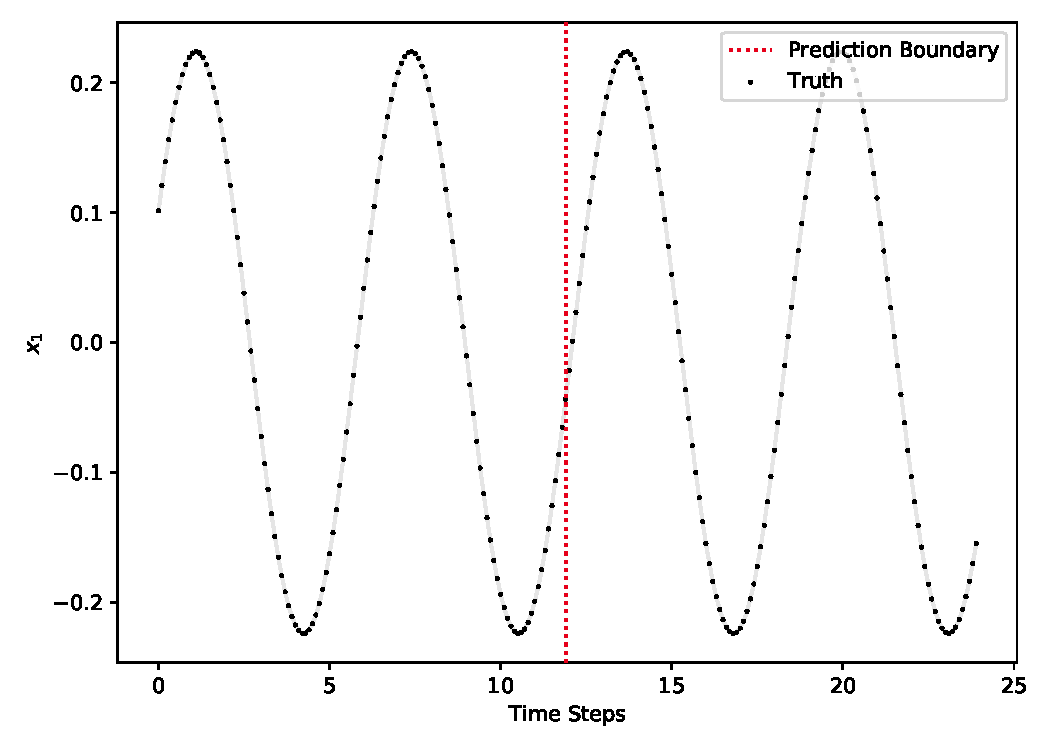
\includegraphics[width=\linewidth]{figures/experiments/environments/observations-lgds-N0-D0.pdf}
			\end{subfigure}%
			~
			\begin{subfigure}{0.5\linewidth}
				\centering
				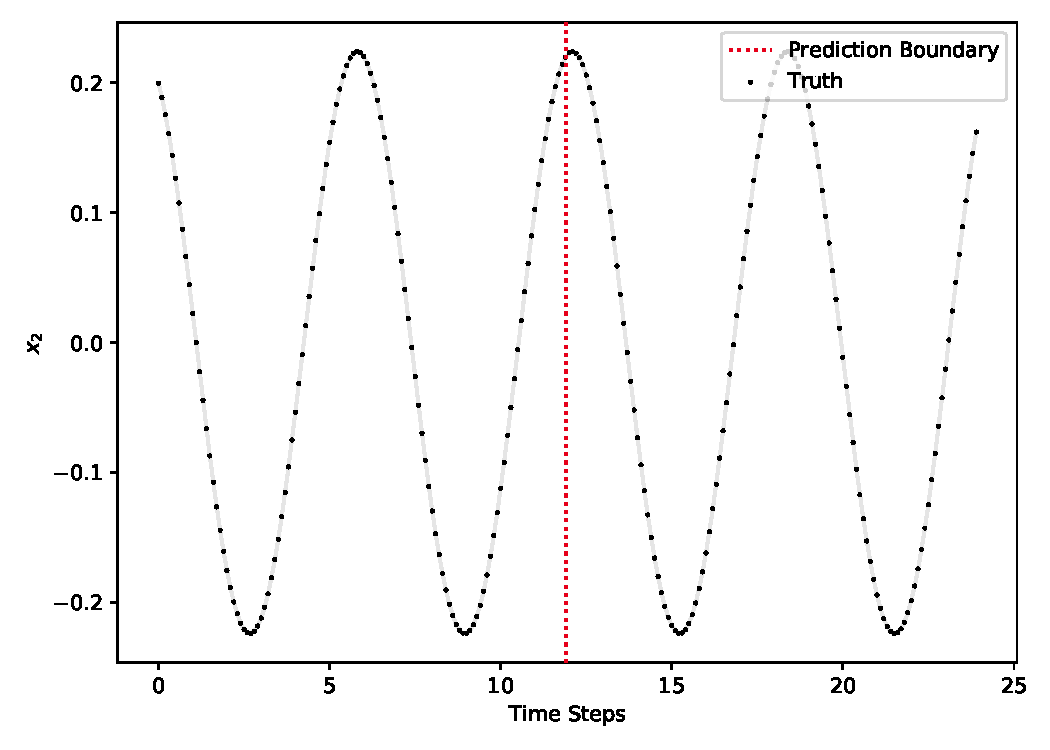
\includegraphics[width=\linewidth]{figures/experiments/environments/observations-lgds-N0-D1.pdf}
			\end{subfigure}
			\caption{Plot of the raw data used for training the proof-of-concept \ac{lgds} environment. The black dots represent the actual data points, all before the red prediction boundary are used for training, the rest for validation. The faint gray line emphasizes the connection between the data points and that they are actually generated from a dynamical system.}
			\label{fig:envLgds}
		\end{figure}
	% end

	\subsection{(Damped) Pendulum}
		\begin{itemize}
			\item Experiment ID: \texttt{pendulum} and \texttt{pendulum\_damped}
		\end{itemize}

		The first nonlinear system we look at is the (inverted) pendulum in both an undamped and a damped setting. For this experiment, we use the angular state \( \vec{y} = \begin{bmatrix} \theta & \dot{\theta} \end{bmatrix} \) where \(\theta\) is the displacement angle (see~\autoref{fig:envPendulumSketch}). The dynamics are specified by the \ac{ode}
		\begin{equation*}
			\ddot{\theta} = \sin\theta - d \dot{\theta}
		\end{equation*}
		that is solved using the Radau~IIA~\cite{guglielmiImplementingRadauIIA2001} \ac{ivp} integrator (after transforming the \ac{ode} in a first-order \ac{ode} system). The initial velocity is set to \(0\) and the initial position is sampled from a Gaussian with mean \( \pi/36 \) and variance \( \pi/8 \). This puts the pendulum in motion as it falls down from its initial position. For the undamped pendulum, we set \( d = 0 \). For both environments, we use an evaluation interval of \( h = 0.1 \) for \( T = 1000 \) time steps where only the first \( T_\train = 500 \) steps are used for training and the remaining \(500\) are used for validation. The raw data is shown in~\autoref{fig:envPendulum} for the undamped and~\autoref{fig:envPendulumDamped} for the damped pendulum.

		The damped pendulum is especially interesting as the system looses energy (\ac{ie} the sum of the kinetic and potential energy decreases over time) and Koopman theory in general has problems with finding embeddings that are able to encode energy loss\todo{citation needed}.

		\begin{figure}
			\centering
			\begin{subfigure}{0.5\linewidth}
				\centering
				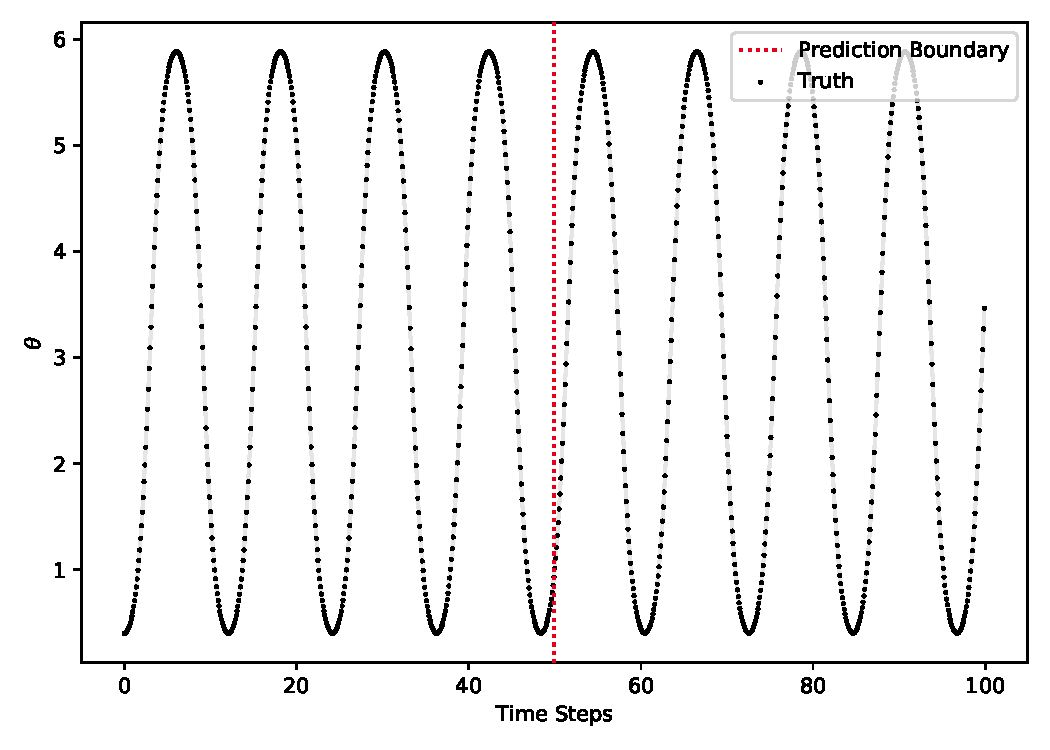
\includegraphics[width=\linewidth]{figures/experiments/environments/observations-pendulum-N0-D0.pdf}
			\end{subfigure}%
			~
			\begin{subfigure}{0.5\linewidth}
				\centering
				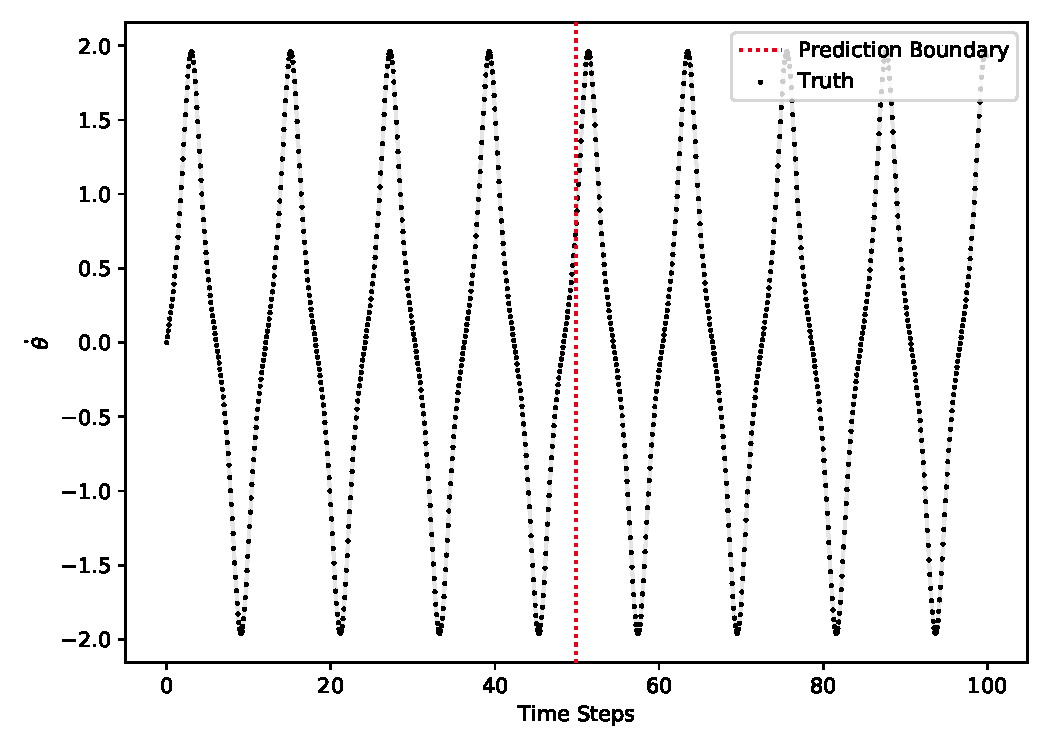
\includegraphics[width=\linewidth]{figures/experiments/environments/observations-pendulum-N0-D1.pdf}
			\end{subfigure}
			\caption{Plot of the raw data used for training the undamped pendulum environment. The black dots represent the actual data points, all before the red prediction boundary are used for training, the rest for validation. The faint gray line emphasizes the connection between the data points and that they are actually generated from a dynamical system.}
			\label{fig:envPendulum}
		\end{figure}
		\begin{figure}
			\centering
			\begin{subfigure}{0.5\linewidth}
				\centering
				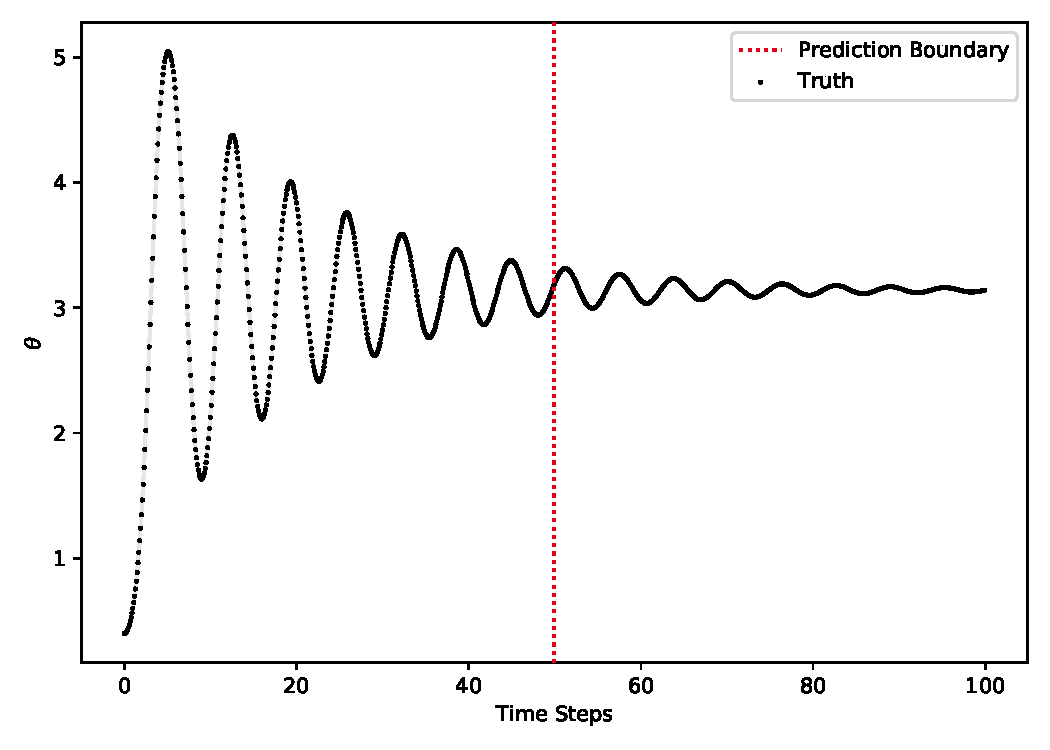
\includegraphics[width=\linewidth]{figures/experiments/environments/observations-pendulum-damped-N0-D0.pdf}
			\end{subfigure}%
			~
			\begin{subfigure}{0.5\linewidth}
				\centering
				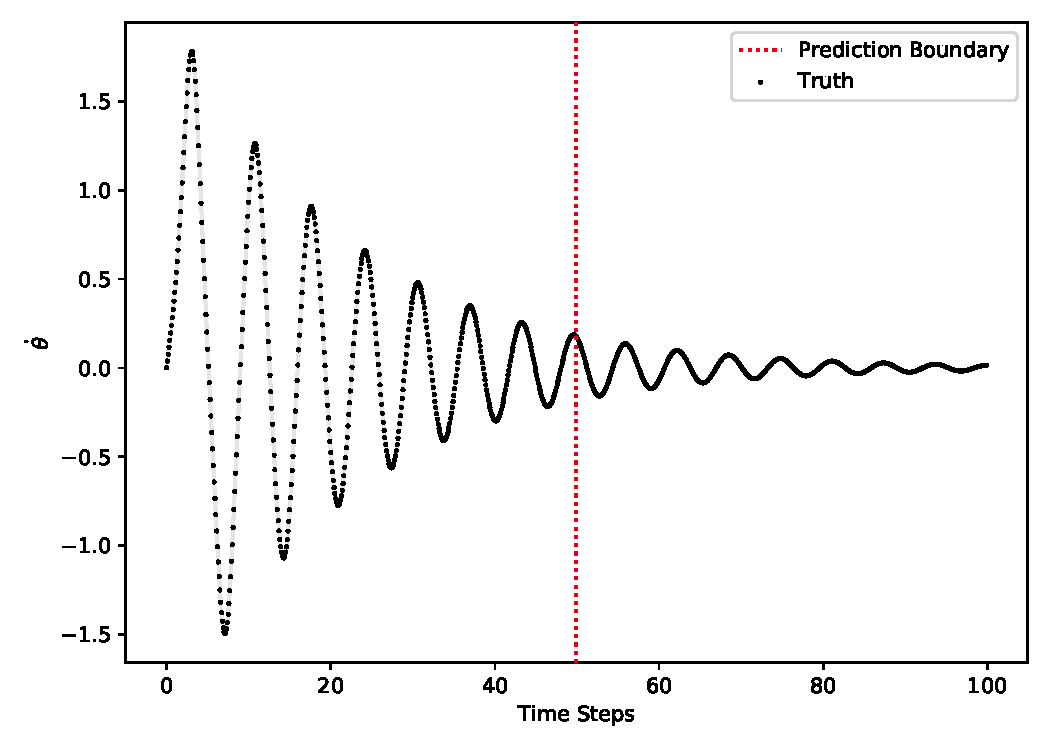
\includegraphics[width=\linewidth]{figures/experiments/environments/observations-pendulum-damped-N0-D1.pdf}
			\end{subfigure}
			\caption{Plot of the raw data used for training the damped pendulum environment. The black dots represent the actual data points, all before the red prediction boundary are used for training, the rest for validation. The faint gray line emphasizes the connection between the data points and that they are actually generated from a dynamical system.}
			\label{fig:envPendulumDamped}
		\end{figure}
	% end

	\subsection{Gym Pendulum}
		\begin{itemize}
			\item Experiment ID: \texttt{pendulum\_gym}
		\end{itemize}

		This is a sine/cosine version of the pendulum introduced before, but without damping. We use the environment of OpenAI Gym~\cite{brockmanOpenAIGym2016} for generating the data used for training. The motion equations are still the same as for the non-Gym pendulum
		\begin{equation*}
			\ddot{\theta} = \sin\theta
		\end{equation*}
		with \( d = 0 \) as the Gym pendulum does not include damping, but the state is defined as the sine and cosine of the angle:
		\begin{equation*}
			\vec{y} \coloneqq
				\begin{bmatrix}
					\cos\theta \\
					\sin\theta \\
					\dot{\theta}
				\end{bmatrix}
		\end{equation*}
		The Gym environment uses the Euler method for integrating the \ac{ode} with a step size of \( h = 0.05 \). We generate \( T = 100 \) time steps of which \( T_\train = 50 \) are used for training and the other \(50\) for validation. The raw data is shown in~\autoref{fig:envPendulumGym}.

		\begin{figure}
			\centering
			\begin{subfigure}{0.5\linewidth}
				\centering
				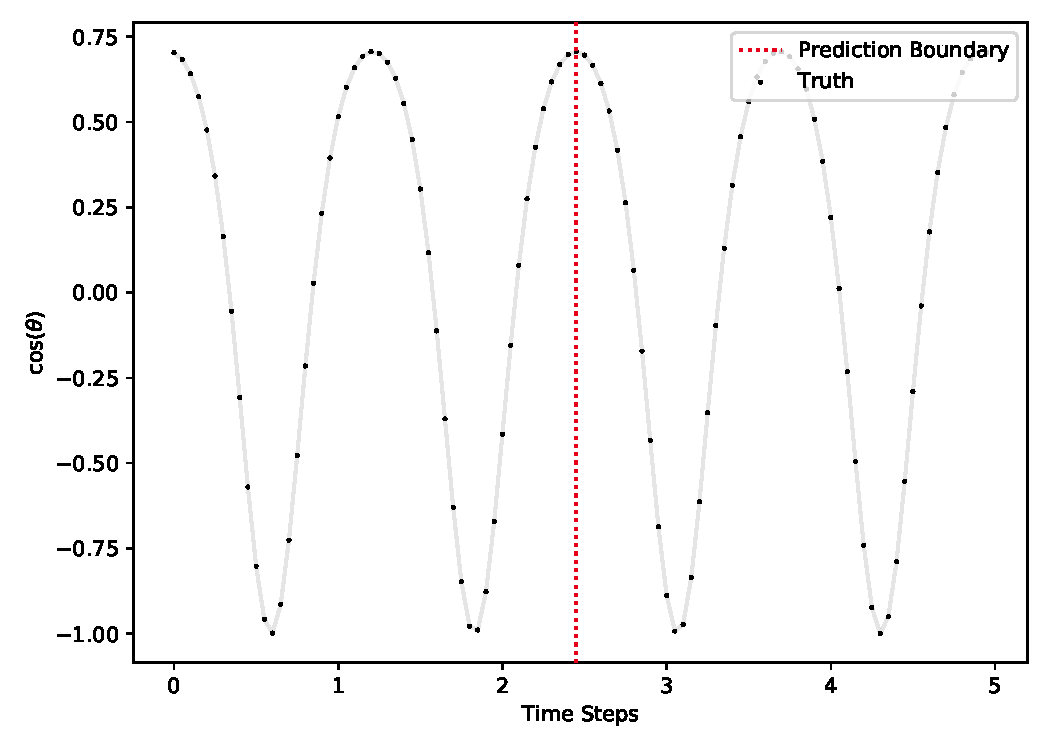
\includegraphics[width=\linewidth]{figures/experiments/environments/observations-pendulum-gym-N0-D0.pdf}
			\end{subfigure}%
			~
			\begin{subfigure}{0.5\linewidth}
				\centering
				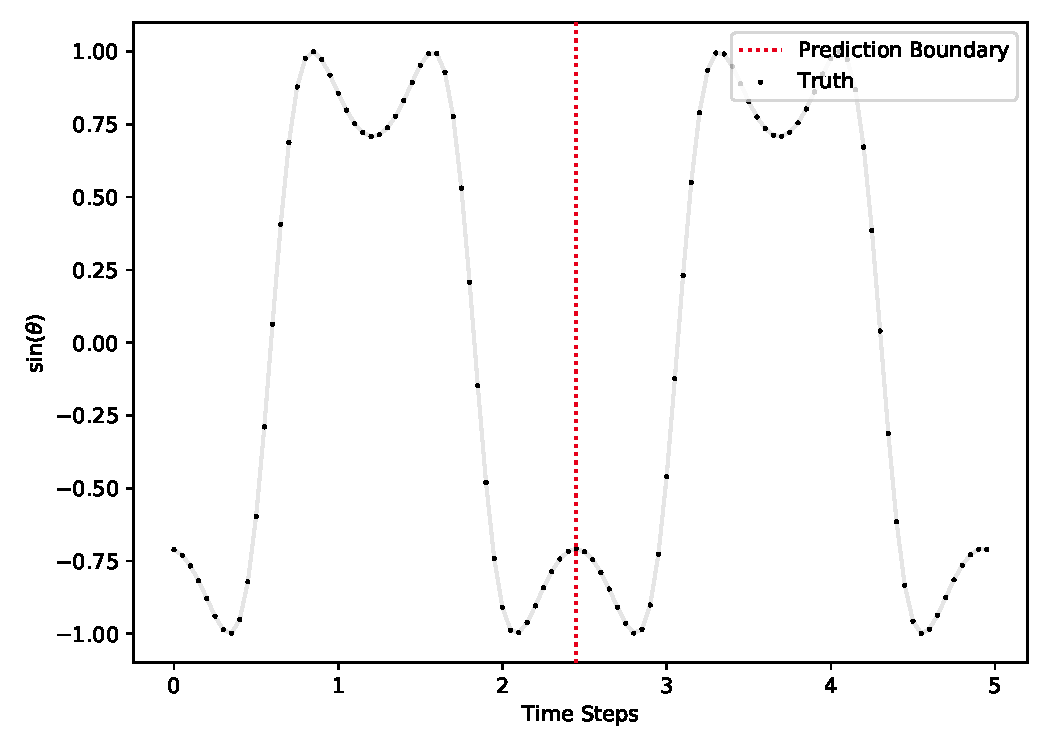
\includegraphics[width=\linewidth]{figures/experiments/environments/observations-pendulum-gym-N0-D1.pdf}
			\end{subfigure} \\
			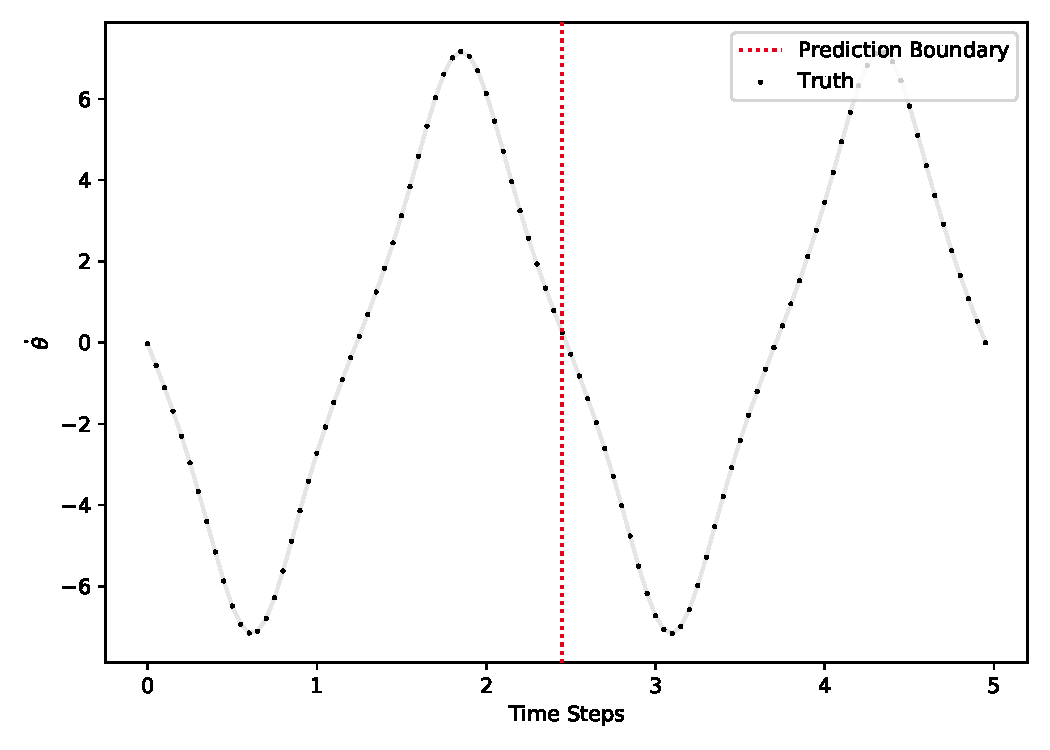
\includegraphics[width=0.5\linewidth]{figures/experiments/environments/observations-pendulum-gym-N0-D2.pdf}
			\caption{Plot of the raw data used for training the Gym pendulum environment. The black dots represent the actual data points, all before the red prediction boundary are used for training, the rest for validation. The faint gray line emphasizes the connection between the data points and that they are actually generated from a dynamical system.}
			\label{fig:envPendulumGym}
		\end{figure}
	% end

	\subsection{Gym Cartpole}
		\begin{itemize}
			\item Experiment ID: \texttt{cartpole\_gym}
		\end{itemize}

		The second last environment we run experiment on is the cartpole environment. In the cartpole environment, an inverted pendulum is build on a (typically controlled, but otherwise freely movable) cart. If the pendulum falls town, the torque on the joint is translated into a force moving the cart around. This creates nonlinear coupling and therefore highly nonlinear dynamics. A sketch of the cartpole environment is given in~\autoref{fig:envCartpoleGymSketch}. As for the previous pendulum, we rely on the cartpole implementation of Gym. We slightly modified the environment to be uncontrolled, as the environment usually has discrete actions for pushing the cart left or right. This modification is shown in~\autoref{lst:uncontrolledCartPole}. The state of the environment is given as
		\begin{equation*}
			\vec{y} \coloneqq
				\begin{bmatrix}
					x \\
					\dot{x} \\
					\theta \\
					\dot{\theta}
				\end{bmatrix}
		\end{equation*}
		where \(x\) is the cart position, \(\dot{x}\) is the cart velocity, \(\theta\) is the pole angle and \(\dot{\theta}\) is the angular velocity. The implemented equations of movement, taken from~\cite{florianCorrectEquationsDynamics2005}, are given as
		\begin{align*}
			\ddot{\theta} &= \frac{g \sin\theta + \cos\theta \Big(\! \frac{-F - m_p \ell \dot{\theta}^2 \sin\theta}{m_c + m_p} \!\Big)}{\ell \Big(\! \frac{4}{3} - \frac{m_p \cos^2\theta}{m_c + m_p} \!\Big)} \\
			\ddot{x} &= \frac{F + m_p \ell \big( \dot{\theta}^2 \sin\theta - \ddot{\theta} \cos\theta \big)}{m_c + m_p}
		\end{align*}
		where \( g = \SI{9.81}{\meter\per\second\squared} \) is the gravitational acceleration, \( m_p = \SI{0.1}{\kilogram} \) and \( m_c = \SI{1}{\kilogram} \) are the masses of the pole and cart, respectively, \( 2\ell = \SI{1}{\meter} \) is the pole length and \( [F] = \si{\newton} \) is the external (control) force acting on the cart that we set to \( \SI{0}{\newton} \). The Gym environment uses the Euler method for integrating the \ac{ode} with a step size of \( h = 0.02 \). We generate \( T = 300 \) time steps of which we use \( T_\train = 150 \) for training and the remaining \(150\) steps for validation. The raw data is shown in~\autoref{fig:envCartpoleGym}.

		\begin{lstlisting}[caption={Modification of Gym's cartpole environment to get an uncontrolled cartpole.}, label=lst:uncontrolledCartPole]
from gym.envs.classic_control import CartPoleEnv

class UncontrolledCartPole(CartPoleEnv):
	def __init__(self):
	super().__init__()

	self.force_mag = 0.0
		\end{lstlisting}

		\begin{figure}
			\centering
			\tikzCartpole
			\caption{Illustration of the cartpole environment. The cart has mass \(m_c\), the pole \(m_p\) with length \(L\). The cart can move freely on the \(x\) axis, while the pendulum can swing freely around the center of the cart, causing it to move.}
			\label{fig:envCartpoleGymSketch}
		\end{figure}

		\begin{figure}
			\centering
			\begin{subfigure}{0.5\linewidth}
				\centering
				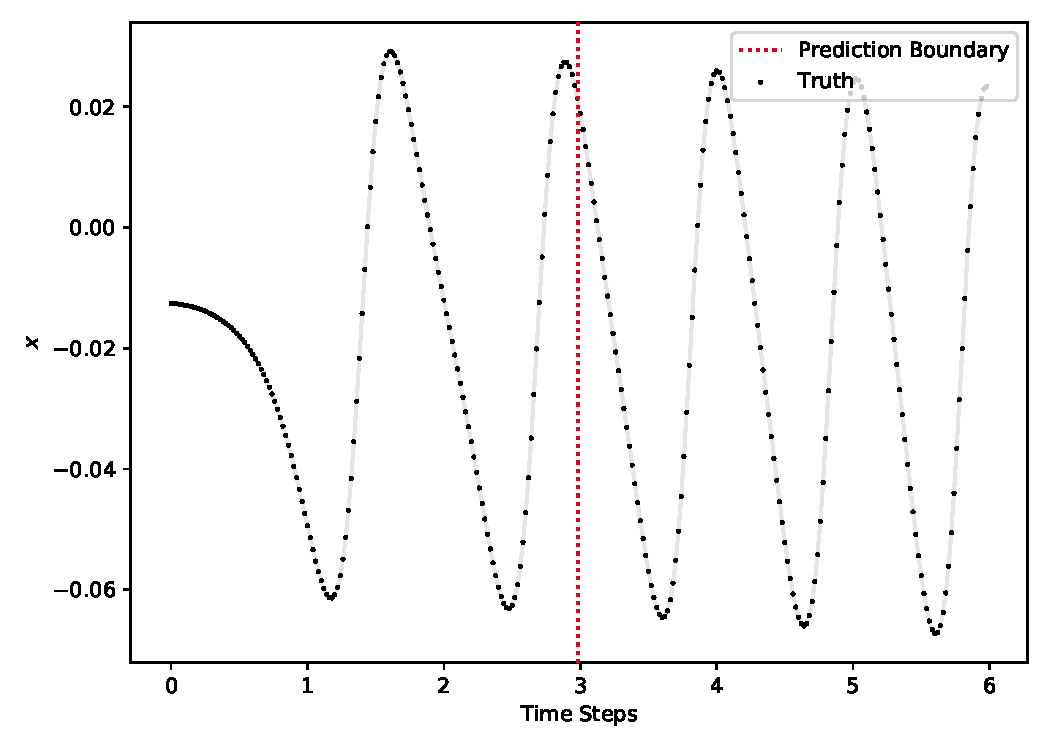
\includegraphics[width=\linewidth]{figures/experiments/environments/observations-cartpole-gym-N0-D0.pdf}
			\end{subfigure}%
			~
			\begin{subfigure}{0.5\linewidth}
				\centering
				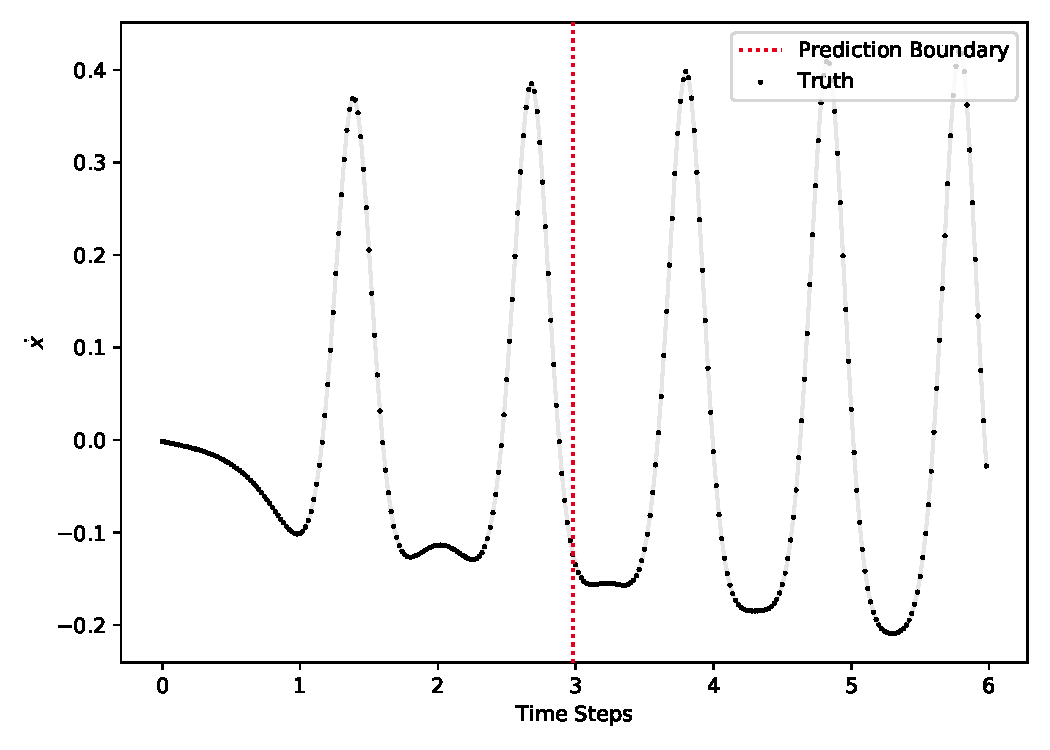
\includegraphics[width=\linewidth]{figures/experiments/environments/observations-cartpole-gym-N0-D1.pdf}
			\end{subfigure} \\
			\begin{subfigure}{0.5\linewidth}
				\centering
				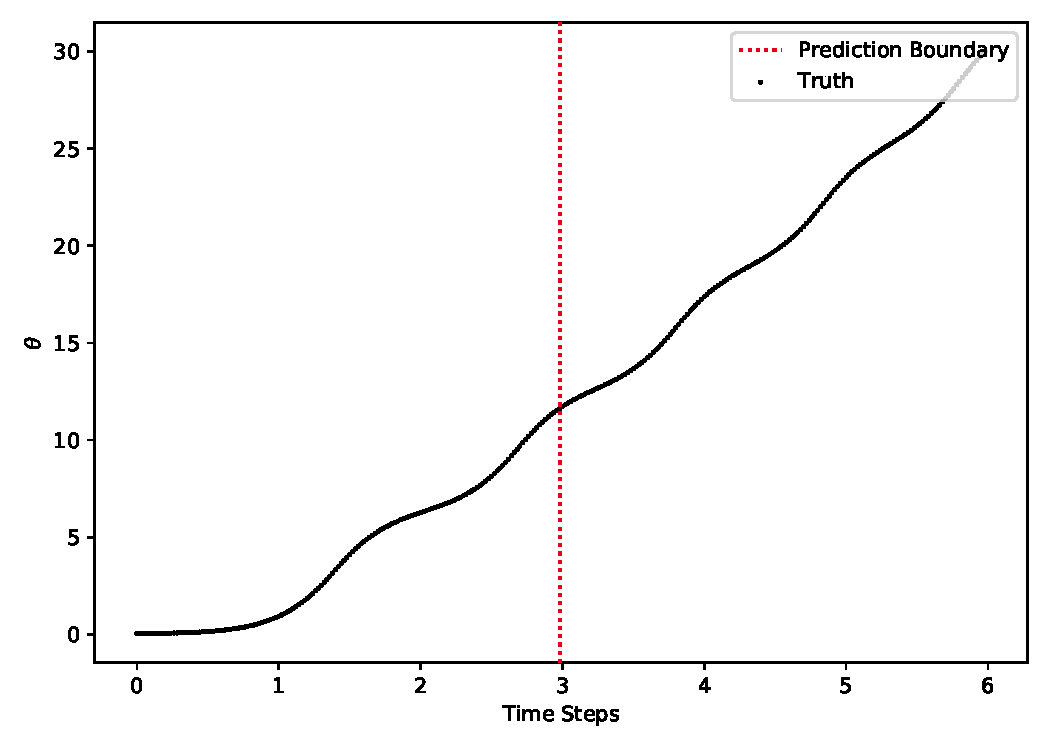
\includegraphics[width=\linewidth]{figures/experiments/environments/observations-cartpole-gym-N0-D2.pdf}
			\end{subfigure}%
			~
			\begin{subfigure}{0.5\linewidth}
				\centering
				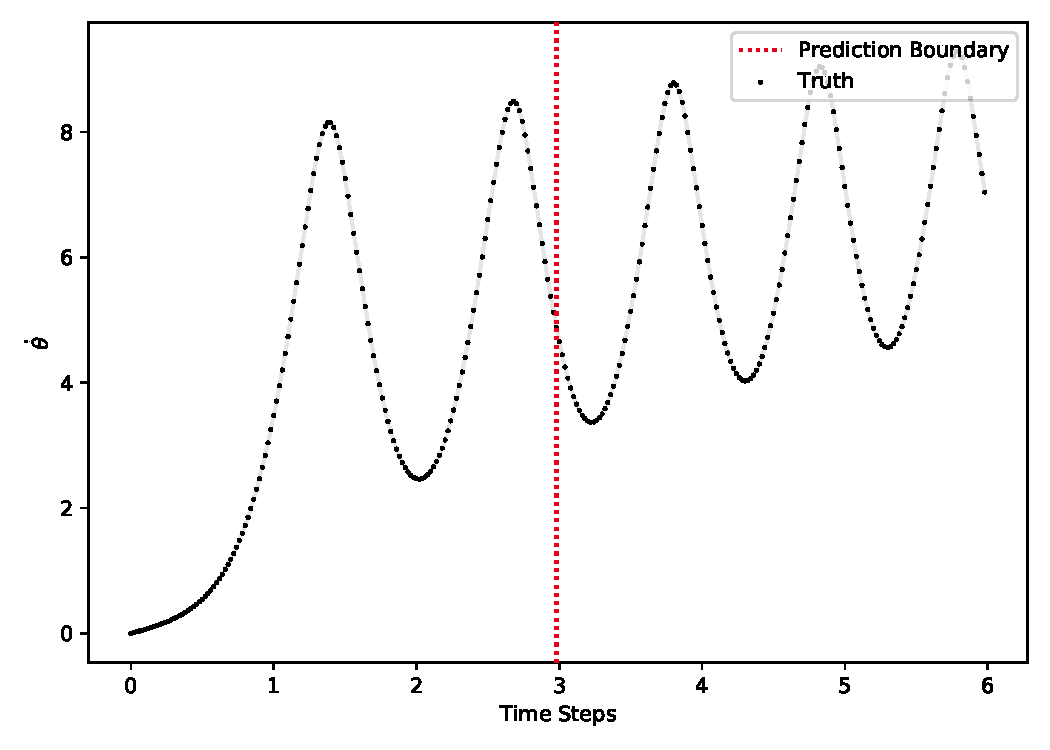
\includegraphics[width=\linewidth]{figures/experiments/environments/observations-cartpole-gym-N0-D3.pdf}
			\end{subfigure}
			\caption{Plot of the raw data used for training the Gym cartpole environment. The black dots represent the actual data points, all before the red prediction boundary are used for training, the rest for validation. The faint gray line emphasizes the connection between the data points and that they are actually generated from a dynamical system.}
			\label{fig:envCartpoleGym}
		\end{figure}
	% end

	\subsection{Gym Double Pendulum}
		\begin{itemize}
			\item Experiment ID: \texttt{acrobot\_gym}
		\end{itemize}

		The last environment we test is the double pendulum, implemented in Gym as the \emph{acrobot} (as for the cartpole, we removed all control inputs and modified the initial state to start on top rather than hanging straight down, see~\autoref{lst:topAcrobot}). The double pendulum consists of a pendulum on a fixed joint and a second pendulum attached to the end of the first pendulum. This creates highly nonlinear coupling and is the most common example of a chaotic system~\cite{shinbrotChaosDoublePendulum1992}. We observe the state vector
		\begin{equation*}
			\vec{y} \coloneqq
				\begin{bmatrix}
					\cos\varphi_1 \\
					\sin\varphi_1 \\
					\cos\varphi_2 \\
					\sin\varphi_2 \\
					\dot{\varphi}_1 \\
					\dot{\varphi}_2
				\end{bmatrix}
		\end{equation*}
		where \(\varphi_1\) and \(\varphi_2\) are the displacement of the first and second joint, respectively. See~\autoref{fig:envDoublePendulumGymSketch}) for a sketch of the double pendulum. The governing equations of motion are given as:´
		\begin{align*}
			\ddot{\varphi}_1 &= \frac{g (\sin\varphi_2 \, \cos\varphi_\Delta - \mu \sin\varphi_1) - (\ell_2 \dot{\varphi}_2^2 + \ell_1 \dot{\varphi}_1^2 \cos\varphi_\Delta) \sin\varphi_\Delta}{\ell_1 (\mu - \cos^2\varphi_\Delta)} \\
			\ddot{\varphi}_2 &= \frac{g \mu (\sin\varphi_2 \, \cos\varphi_\Delta - \mu \sin\varphi_1) + (\mu \ell_1 \dot{\varphi}_1^2 + \ell_2 \dot{\varphi}_2^2 \cos\varphi_\Delta) \sin\varphi_\Delta}{\ell_2 (\mu - \cos^2\varphi_\Delta)}
		\end{align*}
		with \( \varphi_\Delta \coloneqq \varphi_1 - \varphi \), \( \mu \coloneqq 1 + m_1/m_2 \) where \( g = \SI{9.8}{\meter\per\second\squared} \) is the gravitational acceleration, \( m_1 = \SI{1}{\kilogram} \) and \( m_2 = \SI{1}{\kilogram} \) are the masses of the two links and \( \ell_1 = \SI{1}{\meter} \) and \( \ell_2 = \SI{1}{\meter} \) are the lengths of the two links. The Gym environment uses a \ac{rk4} for integrating the \ac{ode} with an evaluation interval of \( h = 0.2 \). We modified the initial position to be drawn from a Gaussian with mean \( \pi \) and standard deviation \( \pi/8 \) and the initial velocity to be drawn from a uniform distribution in the interval \( [-0.1, 0.1] \). We generate \( T = 100 \) time steps of which we use \( T_\train = 75 \) for training and the remaining \(25\) for validation. The raw data is shown in~\autoref{fig:envDoublePendulumGym}.

		\begin{lstlisting}[caption={Modification of Gym's acrobot environment to start at the top instead of hanging down.}, label=lst:topAcrobot]
import numpy as np
from gym.envs.classic_control import AcrobotEnv

class ModifiedAcrobotEnv(AcrobotEnv):
	def __init__(self):
		super().__init__()

	def reset(self):
		position = self.np_random.normal(np.pi, np.pi / 8.0, size=(2,))
		velocity = self.np_random.uniform(low=-0.1, high=0.1, size=(2,))
		self.state = np.concatenate([position, velocity], axis=0)
		return self._get_ob()
		\end{lstlisting}

		\begin{figure}
			\centering
			\tikzDoublePendulum
			\caption{Illustration of the double pendulum environment. The pendulums have lengths \(\ell_1\) and \(\ell_2\) with the masses \(m_1\) and \(m_2\) attached to the respective ends. The inner pendulum can swing freely around the center while the other pendulum can swing freely around the end of the inner pendulum. Hence fixing one of the pendulums would transform the system back to a simple pendulum. If both pendulums can swing, the system is chaotic.}
			\label{fig:envDoublePendulumGymSketch}
		\end{figure}

		\begin{figure}
			\centering
			\begin{subfigure}{0.5\linewidth}
				\centering
				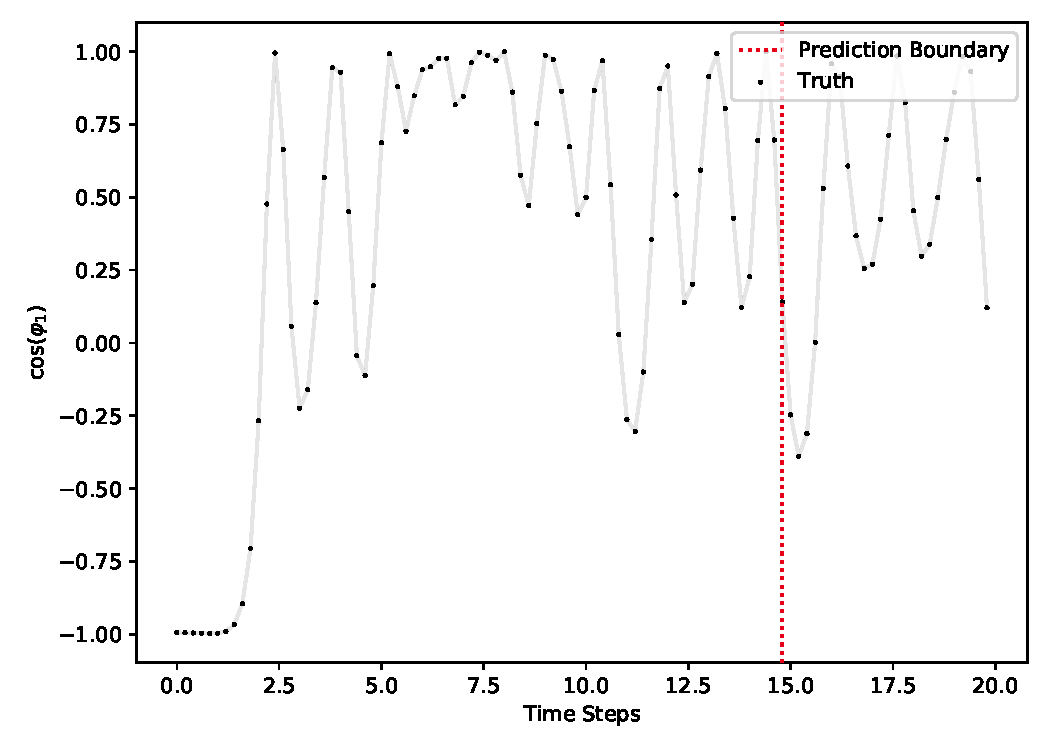
\includegraphics[width=\linewidth]{figures/experiments/environments/observations-acrobot-gym-N0-D0.pdf}
			\end{subfigure}%
			~
			\begin{subfigure}{0.5\linewidth}
				\centering
				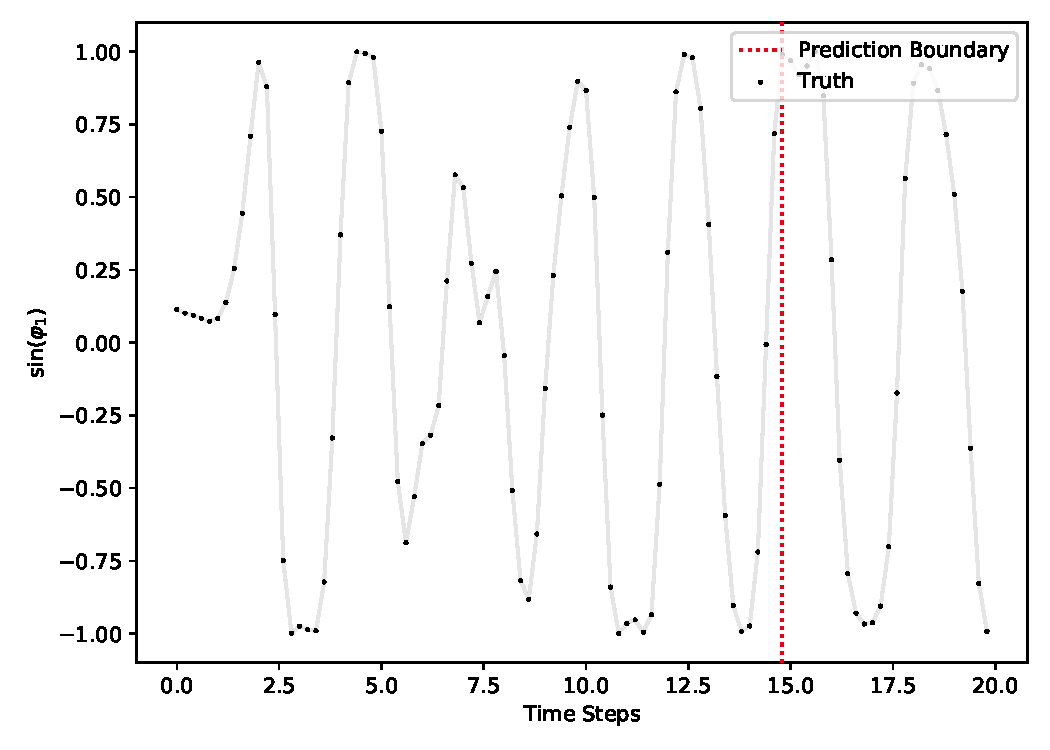
\includegraphics[width=\linewidth]{figures/experiments/environments/observations-acrobot-gym-N0-D1.pdf}
			\end{subfigure} \\
			\begin{subfigure}{0.5\linewidth}
				\centering
				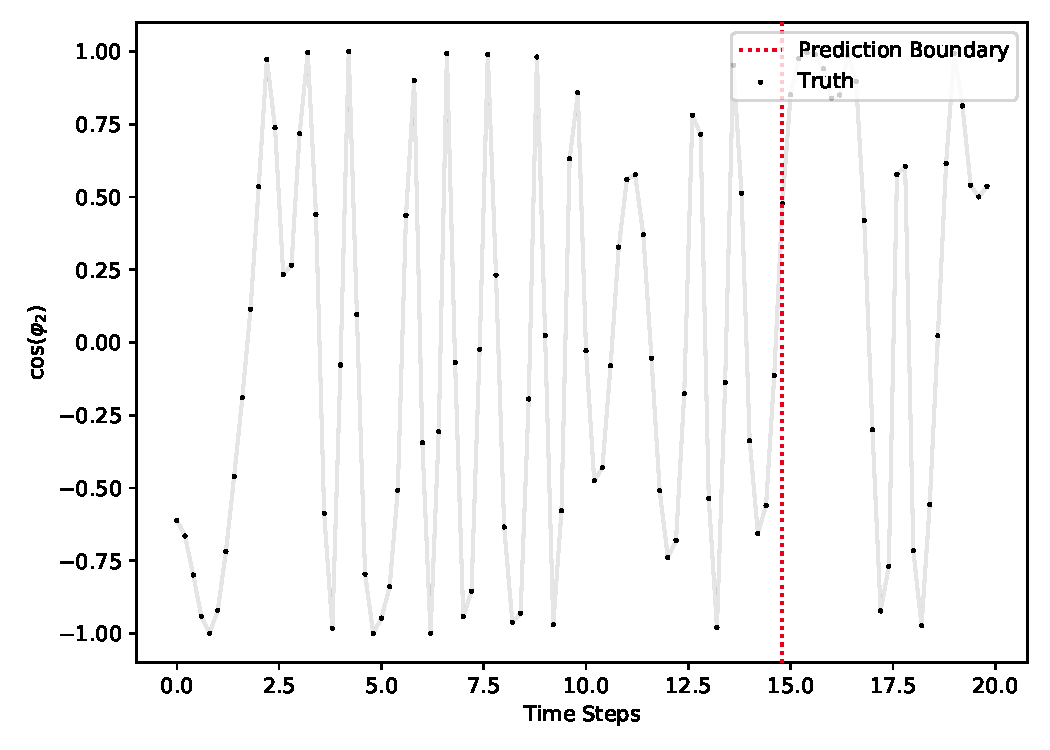
\includegraphics[width=\linewidth]{figures/experiments/environments/observations-acrobot-gym-N0-D2.pdf}
			\end{subfigure}%
			~
			\begin{subfigure}{0.5\linewidth}
				\centering
				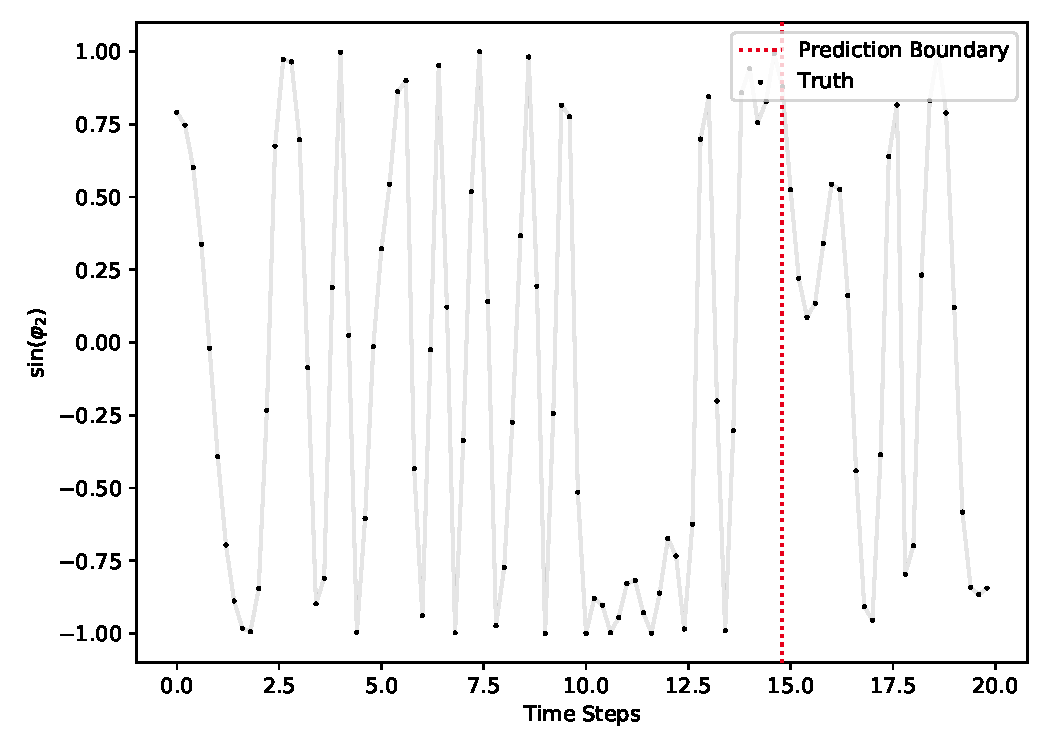
\includegraphics[width=\linewidth]{figures/experiments/environments/observations-acrobot-gym-N0-D3.pdf}
			\end{subfigure} \\
			\begin{subfigure}{0.5\linewidth}
				\centering
				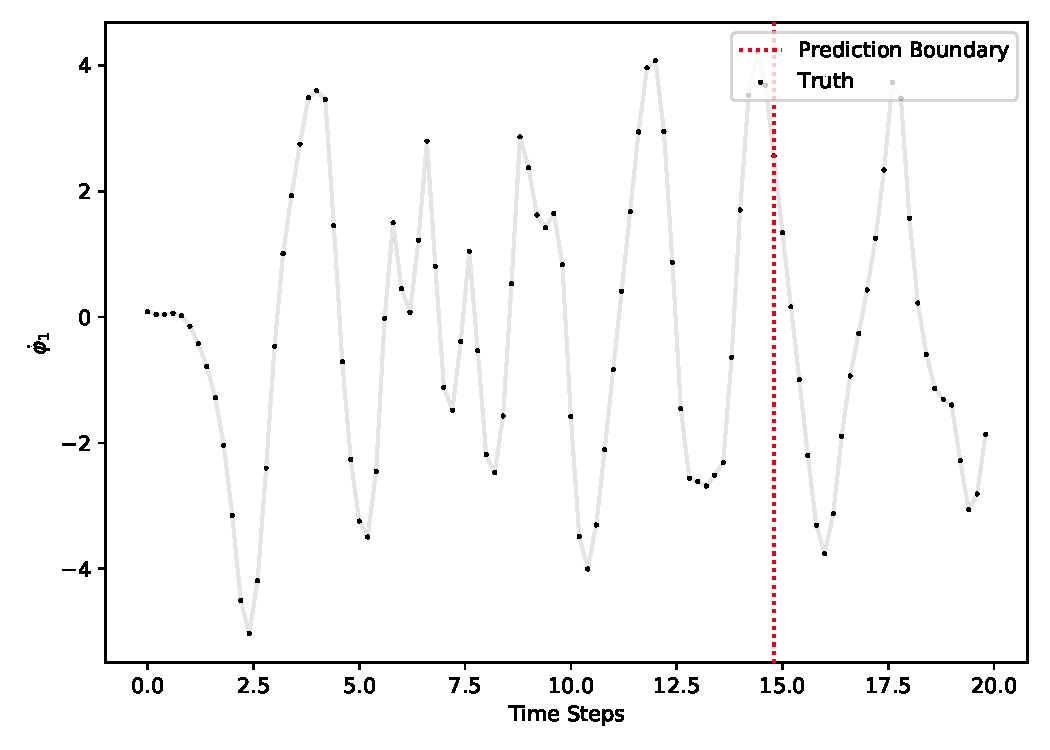
\includegraphics[width=\linewidth]{figures/experiments/environments/observations-acrobot-gym-N0-D4.pdf}
			\end{subfigure}%
			~
			\begin{subfigure}{0.5\linewidth}
				\centering
				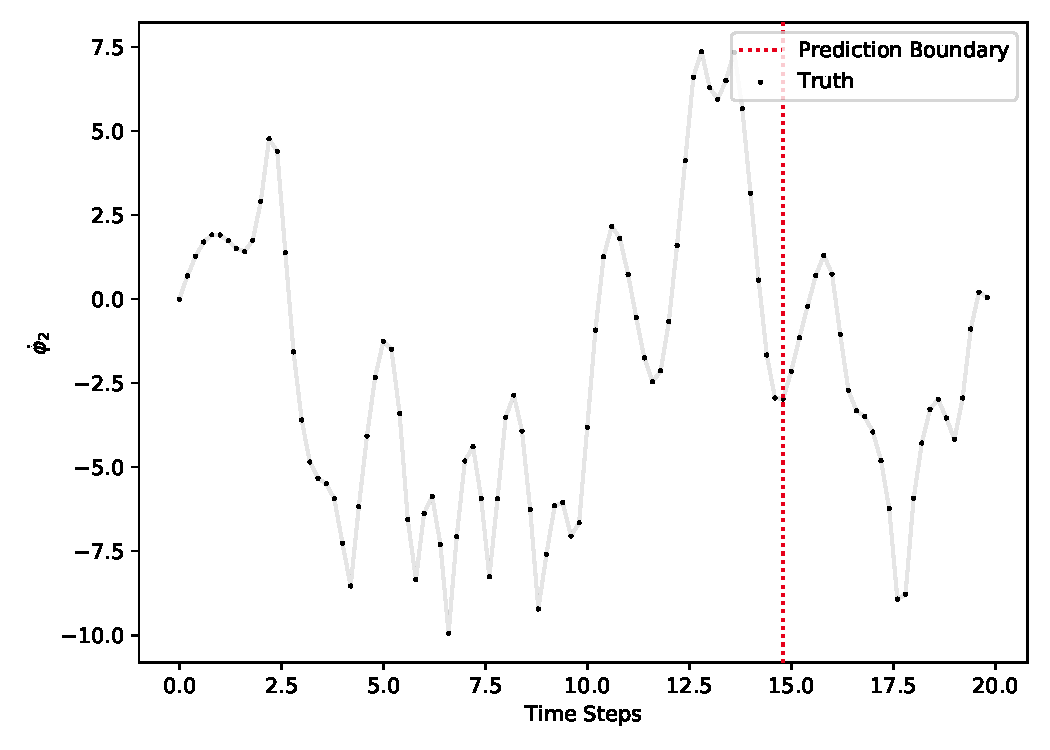
\includegraphics[width=\linewidth]{figures/experiments/environments/observations-acrobot-gym-N0-D5.pdf}
			\end{subfigure}
			\caption{Plot of the raw data used for training the Gym double pendulum environment. The black dots represent the actual data points, all before the red prediction boundary are used for training, the rest for validation. The faint gray line emphasizes the connection between the data points and that they are actually generated from a dynamical system.}
			\label{fig:envDoublePendulumGym}
		\end{figure}
	% end
% end

\section{Experiments with Hyperparameters}
	% Probably more if I can run more experiments… But all other hyperparameters are not as interesting.

	\todo{Exp: Hyper-experiments}

	\subsection{Influence of the Latent Dimensionality}
		\label{subsec:experimentLatentDim}

		\todo{Exp Hyper: Latent Dim}
	% end
% end

	\chapter{Discussion}
\label{c:dicussion}
\IMRADlabel{discussion}



\todo{Experiments}

\section{Performance}
	\todo{Exp: Performance}
% end

\section{Comparison with Related Work}
	% In-Depth Comparison with Lush et al.
	% In-Depth Comparsion with Morton et al.
	% Probably more qualitative comparisons with Sequential VAE or DVBF (Karl et al.).

	\todo{Exp: Comparison}
% end

	\chapter{Conclusion}
\label{c:conclusion}



\todo{Conclusion}

\section{Summary}
	\todo{Conclusion: Summary}
% end

\section{Control}  % Only if there is time left!
	% Introduce approach to control.
	% Show results of LGDS control which is working.
	% Highlight difficulties.

	\todo{Conclusion: Control}
% end

\section{Future Work}
	\label{sec:futureWork}

	% Control
	% Full Bayesian
	% Automatic Relevance Determination (ARD) on Latent Space, see Beal's Variational Kalman Smoother

	\todo{Conclusion: Future Work}
% end


	\cleardoublepage
	\bibliography{literature/lit}
	\nocite{*}

	\cleardoublepage
	\appendix
	\chapter{Invent some nice chapter title} \todo{Chapter title.}
	\section{Solution of the Harmonic Oscillator}
		\label{app:harmonicOscillatorSolution}
	
		To solve the differential motion equation
		\begin{align*}
			m\ddot{x} = -kx
		\end{align*}
		of the harmonic oscillator given in~\autoref{subsec:harmonicOscillator}, we use the solution approach
		\begin{align*}
			x(t) = c e^{\lambda t} \qquad \dot{x}(t) = \lambda c e^{\lambda t} \qquad \ddot{x}(t) = \lambda^2 c e^{\lambda t}
		\end{align*}
		and insert it into the differential equation:
		\begin{align*}
			m\ddot{x} = -kx \quad\implies\quad
			m \lambda^2 c e^{\lambda t} = -k c e^{\lambda t} \quad\iff\quad
			m \lambda^2 = -k \quad\iff\quad
			\lambda = \pm \sqrt{-\frac{k}{m}}
		\end{align*}
		As both \(k\) and \(m\) are defined to be positive, we get the complex solutions:
		\begin{align*}
			x_1(t) = e^{i t \sqrt{k / m}} \qquad x_2(t) = e^{-i t \sqrt{k / m}}
		\end{align*}
		Due to the superposition principle, also \( x_1 + x_2 \) and \( x_1 - x_2 \) are solutions. Hence, we get two real solutions by using Euler's identity \( e^{\varphi i} = \cos(\varphi) + i \sin(\varphi) \):
		\begin{align*}
			x_1 + x_2
				&= e^{i t \sqrt{k / m}} + e^{-i t \sqrt{k / m}} \\
				&= \cos\Big(t \sqrt{k / m}\Big) + i \sin\Big(t \sqrt{k / m}\Big) + \cos\Big(t \sqrt{k / m}\Big) - i \sin\Big(t \sqrt{k / m}\Big) \\
				&= 2 \cos\Big(t \sqrt{k / m}\Big) \\
			x_1 - x_2
				&= e^{i \sqrt{k / m} t} - e^{-i t \sqrt{k / m}} \\
				&= \cos\Big(t \sqrt{k / m}\Big) i \sin\Big(t \sqrt{k / m}\Big) - \cos\Big(t \sqrt{k / m}\Big) + i \sin\Big(t \sqrt{k / m}\Big) \\
				&=  2i \sin\Big(t \sqrt{k / m}\Big)
		\end{align*}
		This yields the following general solution:
		\begin{align*}
			x(t) = c_1 \cos\Big(t \sqrt{k / m}\Big) + c_2 \sin\Big(t \sqrt{k / m}\Big),\quad c_1, c_2 \in \C
		\end{align*}
		As both Sine and Cosine are Sinusoidal, different \( c_1 \neq c_2 \) only lead to a phase shift. Thus we can also write the solution as
		\begin{align*}
			x(t) = A \cos\Big(t \sqrt{k / m} + \varphi\Big)
		\end{align*}
		with the amplitude \(A\) and the phase \(\varphi\).
	% end
% end

	\chapter{Snippets}
		\section{Basics}



\subsection{Dynamical Systems}
	\subsubsection{Koopman Dynamical Systems and the Koopman Operator}
		As we have seen, classical linearization approaches like the small angle approximation are only valid in a narrow section around the linearization point. While this works well for simple control tasks such as swinging up and balancing an inverted pendulum~\cite{bugejaNonlinearSwingupStabilizing2003}, it does not work out for predicting future trajectories of the system. % TODO: Citation needed.

		Consider a first-order, autonomous dynamical system
		\begin{align*}
			\dot{\vec{x}} = \vec{f}(\vec{x}),\quad \vec{f} : \R^n \to \R^n
		\end{align*}
		and observables ("measurements") \( \vec{g} : \R^n \to \R^m \). The Koopman operator \( \mathcal{K} \), an infinite-dimensional linear operator, acts on them as follows:
		\begin{align*}
			\mathcal{K} \vec{g} = \vec{g} \circ \vec{F} \quad\iff\quad \mathcal{K} \vec{g}(\vec{x}_t) = \vec{g}\big(\vec{F}(\vec{x}_t)\big) = \vec{g}(\vec{x}_{t + 1})
		\end{align*}
		In other words, the Koopman operator advances our observables \(\vec{g}\) linearly forward in time. This behavior is illustrated in~\autoref{fig:koopmanOperatorBrunton}.

		The Koopman operator can also be formulated for time-continuous systems~\cite{abrahamManifoldsTensorAnalysis2012}:
		\begin{align*}
			\dv{t} \vec{g} = \mathcal{K} \vec{g}
		\end{align*}

		% TODO: Further explain Koopman theory after reading the corresponding sections in the Abraham book.

		\begin{figure}
			\centering
			\tikzKoopmanOperator
			\caption{Illustration of a Koopman dynamical system where time flows from left to right. The top row shows the linear embedding with the Koopman operator \( \mathcal{K} \) to transition from \(\vec{y}_t\) to \(\vec{y}_{t + 1}\). The bottom row shows the nonlinear dynamics produced by the dynamics function \(\vec{F}\). The measurement function \(\vec{g}\) allows transitioning between the two representations of the system state where \(\vec{g}^{-1}\) describes an "inverse" measurement function to recover the original nonlinear state from the linear embedding. We would like to find such a function. Adopted from~\cite{bruntonKoopmanInvariantSubspaces2016}.}
			\label{fig:koopmanOperatorBrunton}
		\end{figure}
	% end
% end

\subsection{Hidden Markov Models and Linear Gaussian Dynamical Systems}
	\subsubsection{Hidden Markov Models}
		\label{subsec:hiddenMarkovModel}

		\acp{hmm} are simple Bayesian networks described by a non-observable (\emph{hidden}) Markov chain. This non-observable discrete chain can be indirectly observed with measurements that are emitted by every state. One of the key features of a Markov chain is that a state does only depend on the previous state, but not on the second previous, third previous, and so on, states. That is, knowing only the previous state is sufficient and no more information can be gathered by knowing every other state before. This is described by the state transition distribution
		\begin{align*}
			s_{k + 1} \sim p(s_{k + 1} \given s_k)
		\end{align*}
		being only dependent on the previous state \(s_k\). Analogous, a measurement \(\vec{y}_k\) of a state \(s_k\) is only dependent on that specific state:
		\begin{align*}
			\vec{y}_k \sim p(\vec{y}_k \given s_k)
		\end{align*}
		These assumptions are called the \emph{Markov property} and a system fulfilling this property is called \emph{Markovian}. These conditional distributions can be written in a graphical model as shown in~\autoref{fig:hiddenMarkovModel}. Note that, in general, no assumption has to be made on the "type" of state/observation (\ac{ie} whether it is a scalar, a vector or something completely different). Also, no assumption is made on the specific transition distributions, \acp{hmm} can also be used to model deterministic transitions using a Dirac delta distribution.

		\begin{figure}
			\centering
			\tikzHiddenMarkovModel
			\caption{Illustration of a completely general Hidden Markov Model with states \(s_k\) and emissions/observations \(\vec{y}_k\).}
			\label{fig:hiddenMarkovModel}
		\end{figure}
	% end

	\subsubsection{Linear Gaussian Dynamical Systems}
		A general time-discrete linear system is described by a state transition
		\begin{align*}
			\vec{x}_{t + 1} = \mat{A} \vec{x}_t
		\end{align*}
		with a dynamics matrix \(\mat{A}\). Using purely additive Gaussian zero-mean noise \( \vec{\epsilon} \sim \normal(\vec{0}, \mat{Q}) \) with covariance matrix \( \mat{Q} \), the state transition becomes probabilistic:
		\begin{align*}
			\vec{x}_{t + 1} = \mat{A} \vec{x}_t + \vec{\epsilon} \quad\iff\quad \vec{x}_{t + 1} \sim \normal(\mat{A} \vec{x}_t, \mat{Q})
		\end{align*}
		With analogously defined measurements,
		\begin{align*}
			\vec{y}_t \sim \normal(\mat{C} \vec{x}_t, \mat{R})
		\end{align*}
		the dynamical system becomes a \ac{lgds}, which is very similar to the \ac{hmm} described in~\autoref{subsec:hiddenMarkovModel}. It can also be represented using a graphical model as shown in~\autoref{fig:lgds}. In fact, a \ac{lgds} is kind of a \ac{hmm}, except the states are not discrete but continuous.

		\begin{figure}
			\centering
			\tikzLinearGaussianDynamicalSystem
			\caption{Illustration of a Linear Gaussian Dynamical System with states \(\vec{x}_t\) and observations \(\vec{y}_t\). Solid arrows represent probabilistic dependency, where the matrix \(\mat{A}\) is the dynamics matrix indicating that the mean transitions linearly, so do the observations with the observation matrix \(\mat{C}\).}
			\label{fig:lgds}
		\end{figure}
	% end

	\subsubsection{Inference}
		% TODO: Stopped here.
	% end
% end

\subsection{The Expectation-Maximization Algorithm}
	The \ac{em} algorithm, first introduced by Ceppellini et al. in 1955~\cite{ceppelliniEstimationGeneFrequencies1955} and popularized by Dempster et al. in 1977~\cite{dempsterMaximumLikelihoodIncomplete1977}, can be used for tackling the following optimization problem: Assuming some model with latent (hidden) states \(\vec{x}\), observations \(\vec{y}\) and model parameters \(\vec{\theta}\), we want to maximize the likelihood \( p(\vec{y} \given \vec{\theta}) \) \ac{wrt} the latent states \(\vec{x}\) and the parameters \(\vec{\theta}\). However, the marginal distribution
	\begin{align*}
		p(\vec{y} \given \vec{\theta}) = \int\! p(\vec{x}, \vec{y} \given \vec{\theta}) \dd{\vec{x}}
	\end{align*}
	is generally intractable. As usual on maximum likelihood approaches, it is useful to not maximize the likelihood directly, but to maximize the log-likelihood
	\begin{align*}
		\mathcal{L}(\vec{\theta}) \coloneqq \log p(\vec{y} \given \vec{\theta}) = \log \int\! p(\vec{x}, \vec{y} \given \vec{\theta}) \dd{\vec{x}}
	\end{align*}
	instead. This yields the same maximum as the logarithm is strictly increasing. By introducing an auxiliary probability distribution \( q(\vec{x} \given \vec{y}) \) over the latent variables, we can rewrite the marginal and find a lower bound on \(\mathcal{L}\) by using Jensen's inequality~\cite{jensenFonctionsConvexesInegalites1906}:
	\begin{align}
		\mathcal{L}(\vec{\theta})
			&= \log \int\! p(\vec{x}, \vec{y} \given \vec{\theta}) \dd{\vec{x}}  \nonumber \\
			&= \log \int\! q(\vec{x} \given \vec{y}) \frac{p(\vec{x}, \vec{y} \given \vec{\theta})}{q(\vec{x} \given \vec{y})} \dd{\vec{x}}  \nonumber \\
			&\geq \int\! q(\vec{x} \given \vec{y}) \log \frac{p(\vec{x}, \vec{y} \given \vec{\theta})}{q(\vec{x} \given \vec{y})} \dd{\vec{x}}  \nonumber \\
			&= \int\! q(\vec{x} \given \vec{y}) \log p(\vec{x}, \vec{y} \given \vec{\theta}) \dd{\vec{x}} - \int\! q(\vec{x} \given \vec{y}) \log q(\vec{x} \given \vec{y}) \dd{\vec{x}} \eqqcolon \mathcal{L}_\mathrm{EM}[q, \vec{\theta}]  \label{eq:emLowerBound}
	\end{align}
	This draws a lower bound \( \mathcal{L}_\mathrm{EM}[q, \vec{\theta}] \) on the log-likelihood \( \mathcal{L}(\vec{\theta}) \) we can maximize instead, maximizing the log-likelihood simultaneously. Note that this lower bound is in fact a functional of the distribution \( q(\vec{x} \given \vec{y}) \).

	The \ac{em} algorithm now iteratively maximizes the lower bound and thus indirectly maximizes the original objective, the likelihood \( p(\vec{y} \given \vec{\theta}) \). The E and M step are as follows:
	\begin{description}
		\item[E-Step] Infers the auxiliary distribution \( q(\vec{x} \given \vec{y}) \) using the current estimations of the parameters \( \vec{\theta} \) by maximizing the lower bound \ac{wrt} the auxiliary distribution.
		\item[M-Step] Infers the parameters \(\vec{\theta}\) using the current auxiliary distribution by maximizing the lower bound \ac{wrt} the parameters.
	\end{description}
	Expressed in equations with the index \( \cdot^{(n)} \) to denote the values of the \(n\)-th iteration, we get the procedure which will be repeated until convergence:
	\begin{description}
		\item[E-Step] \eqparbox[r]{emSteps}{\(\displaystyle q^{(n + 1)} \)} \(\displaystyle = \arg\max_{q}\, \mathcal{L}_\mathrm{EM}\big[ q, \vec{\theta}^{(n)} \big] \)
		\item[M-Step] \eqparbox[r]{emSteps}{\(\displaystyle \vec{\theta}^{(n + 1)} \)} \(\displaystyle = \arg\max_{\vec{\theta}}\, \mathcal{L}_\mathrm{EM}\big[ q^{(n + 1)}, \vec{\theta} \big] \)
	\end{description}
	Additionally, the E-step has the constraint that \(q(\vec{x} \given \vec{y})\) really is a probability distribution, so it must integrate to one:
	\begin{align*}
		\int\! q(\vec{x} \given \vec{y}) \dd{\vec{x}} = 1
	\end{align*}
	We can incorporate this into the maximization, \ac{eg} using Lagrange multipliers. Using a bit of variational calculus, it can be shown~\cite{bealVariationalAlgorithmsApproximate2003} that the maximization is gained by choosing the auxiliary distribution \(q(\vec{x} \given \vec{y})\) to be the same as the distribution \( p(\vec{x} \given \vec{y}, \vec{\theta}) \). That is, we set
	\begin{align*}
		q^{(n + 1)}(\vec{x} \given \vec{y}) = p\big(\vec{x} \biggiven \vec{y}, \vec{\theta}^{(n)}\big)
	\end{align*}
	while holding the parameters \(\vec{\theta}\) fixed. This maximization turns the lower bound into an equality with the actual likelihood~\cite{bealVariationalAlgorithmsApproximate2003}.

	For the M-step, we keep the auxiliary distribution fixed and maximize the lower bound \ac{wrt} the parameters \(\vec{\theta}\). As this involves taking the derivative of \(\mathcal{L}_\mathrm{EM}\) \ac{wrt} \(\vec{\theta}\), we can safely omit the right hand side of the lower bound as it does not depend on \(\vec{\theta}\). Hence, we get the M-step as:
	\begin{align*}
		\vec{\theta}^{(n + 1)}
			&= \arg\max_{\vec{\theta}}\, \mathcal{L}_\mathrm{EM}\big[ q^{(n)}, \vec{\theta} \big] \\
			&= \arg\max_{\vec{\theta}} \int\! q^{(n)}(\vec{x} \given \vec{y}) \log p(\vec{x}, \vec{y} \given \vec{\theta}) \dd{\vec{x}} \\
			&= \arg\max_{\vec{\theta}} \int\! p\big(\vec{x} \biggiven \vec{y}, \vec{\theta}^{(n)}\big) \log p(\vec{x}, \vec{y} \given \vec{\theta}) \dd{\vec{x}} \\
			&= \arg\max_{\vec{\theta}}\, \E_{p\big(\vec{x} \given \vec{y}, \vec{\theta}^{(n)}\big)}[\log p(\vec{x}, \vec{y} \given \vec{\theta})]
	\end{align*}
	The quantity to optimize, \( Q(\vec{\theta}) \coloneqq \E[\log p(\vec{x}, \vec{y} \given \vec{\theta})] \), is also called the \emph{expected complete log-likelihood} as it involves both the observables and the latent variables.

	As shown in~\cite{bealVariationalAlgorithmsApproximate2003}, the lower bound turns into an equality after the E-step. Hence we are guaranteed to always rise the log-likelihood after each \ac{em} iteration if we do not already have the optimal auxiliary distribution and parameters. If this would be the case, both the E- and the M-step would not change anything, so our log-likelihood is monotonically increasing. Also we might not want to calculate the whole distribution in the E-step, but we might want to restrict our computations to sufficient statistics that cover our whole distribution. This procedure may include constraining our auxiliary distribution to some kind of parametric family, \ac{eg} a Gaussian. The procedure for the \ac{em} algorithm is analogous, but the lower bound does not turn into an equality after the E-step, see~\cite[49-51]{bealVariationalAlgorithmsApproximate2003} for more details.

	For the rest of this thesis, we know our distribution \( p(\vec{x} \given \vec{y}, \vec{\theta}) \) is Gaussian, so we can assume the auxiliary distribution to be Gaussian too, given that we set them equal. Hence, we only need to calculate the mean and correlation or covariance of each variable to cover the whole distribution and to be able to proceed. This will turn out to be really useful later on.
% end

\subsection{Variational Autoencoders and the Evidence Lower Bound}
	\acp{vae} have been first introduced in the context of the \ac{aevb} algorithm by Kingma and Welling in 2014~\cite{kingmaAutoEncodingVariationalBayes2014}. They tackle inference and learning in probabilistic models with latent variables, similar to the \ac{em} algorithm. To keep the notation analogous to the derivation of the \ac{em} algorithm, we deviate from~\cite{kingmaAutoEncodingVariationalBayes2014} in terms that we keep \(\vec{x}\) as our latent variables and \(\vec{y}\) as the observables.

	To perform inference, we want to maximize the (log-) likelihood
	\begin{align*}
		\mathcal{L}(\vec{\theta}) \coloneqq \log p(\vec{y} \given \vec{\theta}) = \int\! p(\vec{x}, \vec{y} \given \vec{\theta}) \dd{\vec{x}}
	\end{align*}
	by maximizing the \ac{elbo} \( \mathcal{L}_\mathrm{ELBO} \) which we can find by using Jensen's inequality~\cite{jensenFonctionsConvexesInegalites1906}:
	\begin{align}
		\mathcal{L}(\vec{\theta})
			&= \log \int\! p(\vec{x}, \vec{y} \given \vec{\theta}) \dd{\vec{x}}  \nonumber \\
			&= \log \int\! q(\vec{x} \given \vec{y}, \vec{\phi}) \frac{p(\vec{x}, \vec{y} \given \vec{\theta})}{q(\vec{x} \given \vec{y}, \vec{\phi})} \dd{\vec{x}}  \nonumber \\
			&\geq \int\! q(\vec{x} \given \vec{y}, \vec{\phi}) \log \frac{p(\vec{x}, \vec{y} \given \vec{\theta})}{q(\vec{x} \given \vec{y}, \vec{\phi})} \dd{\vec{x}}  \nonumber \\
			&= \int\! q(\vec{x} \given \vec{y}, \vec{\phi}) \log \frac{p(\vec{y} \given \vec{x}, \vec{\theta}) p(\vec{x} \given \vec{\theta})}{q(\vec{x} \given \vec{y}, \vec{\phi})} \dd{\vec{x}}  \nonumber \\
			&= \int\! q(\vec{x} \given \vec{y}, \vec{\phi}) \frac{p(\vec{y} \given \vec{x}, \vec{\theta})}{q(\vec{x} \given \vec{y}, \vec{\phi})} \dd{\vec{x}} + \int\! q(\vec{x} \given \vec{y}, \vec{\phi}) p(\vec{y} \given \vec{x}, \vec{\theta}) \dd{\vec{x}}  \nonumber \\
			&= -\KL{q(\vec{x} \given \vec{y}, \vec{\phi})}{p(\vec{y} \given \vec{x}, \vec{\theta})} + \E_{q(\vec{x} \given \vec{y}, \vec{\phi})}[p(\vec{y} \given \vec{x}, \vec{\theta})] \eqqcolon \mathcal{L}_\mathrm{ELBO}(\vec{\theta}, \vec{\psi})  \label{eq:elbo}
	\end{align}
	Note that we have introduced an auxiliary parametric distribution \( q(\vec{x} \given \vec{y}, \vec{\phi}) \) which originally leads to the first integral to be an expectation and makes the application of Jensen's inequality possible. We now seek to maximize the \ac{elbo}~\eqref{eq:elbo} \ac{wrt} the variational and generative parameters \(\vec{\phi}\) and \(\vec{\theta}\), respectively. But the gradient \ac{wrt} \(\vec{\phi}\) is problematic, as the usual naive Monte Carlo estimator exhibits very high variance~\cite{kingmaAutoEncodingVariationalBayes2014,paisleyVariationalBayesianInference2012a}.

	They propose a solution to this problem called the \emph{reparametrization trick}. Instead of sampling the latent state \( \tilde{\vec{x}} \sim q(\vec{x} \given \vec{y}, \vec{\phi}) \) directly, a (differentiable) transformation \( \vec{g}_{\varphi}(\vec{\epsilon}, \vec{y}) \) with an auxiliary noise variable \(\vec{\epsilon} \sim p(\vec{\epsilon})\) such that \( \tilde{\vec{x}} = \vec{g}_{\vec{\phi}}(\vec{\epsilon}, \vec{y}) \). By sampling the noise \(\vec{\epsilon}\) and applying the transformation \(\vec{g}_{\vec{\phi}}\), the expectation of some function \( \vec{f}(\vec{x}) \) can be easily calculated with Monte Carlo estimates~\cite{kingmaAutoEncodingVariationalBayes2014} which allows the gradients to flow through the expectation:
	\begin{align*}
		\E_{q_{\vec{\phi}}(\vec{x} \subgiven \vec{y})} [\vec{f}(\vec{x})]
			= \E_{p(\vec{\epsilon})}\big[ \vec{f}(\vec{g}_{\vec{\phi}}(\vec{\epsilon}, \vec{x})) \big]
			\approx \frac{1}{L} \sum_{l = 1}^{L} \vec{f}\big(\vec{g}_{\vec{\phi}}(\vec{\epsilon}^{(l)}, \vec{x})\big),\quad \vec{\epsilon}^{(l)} \sim p(\vec{\epsilon})
	\end{align*}
	This transformation is really simple for a multivariate Gaussian distribution \( \vec{x} \sim \normal(\vec{\mu}, \vec{\sigma}^2 \mat{I}) \) with diagonal covariance, where the reparametrization is just \( \vec{g}_{\vec{\phi}}(\vec{\epsilon}, \vec{y}) = \vec{\mu} + \vec{\sigma} \odot \vec{\epsilon} \) with \( \vec{\epsilon} \sim \normal(\vec{0}, \mat{I}) \) and the element-wise product \( \odot \), also known as the Hadamard product. See~\cite[5]{kingmaAutoEncodingVariationalBayes2014}.

	Shifting to Variational Auto-Encoders, we now represent the auxiliary distribution \( q(\vec{x} \given \vec{y}, \vec{\phi}) \) using a neural network with some prior \( p(\vec{x} \given \vec{\theta}) \), e.g. a standard Gaussian \( p(\vec{x} \given \vec{\theta}) = \normal(\vec{0}, \mat{I}) \) to keep the latents "close to the center". This neural network, called the \emph{amortization network}, produces the mean and the diagonal covariance of \( q(\vec{x} \given \vec{y}, \vec{\phi}) \) and computing the expectation is done using the Monte Carlo sampling method combined with the reparametrization trick. A second neural network is used for decoding the latent dimension, representing the decoding distribution \( p(\vec{y} \given \vec{x}, \vec{\theta}) \). If we assume a Gaussian decoding distribution with constant variance, the right side of the \ac{elbo}~\eqref{eq:elbo} just becomes the squared error between the decoding mean and the input \(\vec{y}\). Typically, we assume a smaller dimension of \(\vec{x}\) (the \emph{latent dimension}) than \( \vec{y} \) (the \emph{observation dimension}) to enforce an encoding of the observations and possibly find smaller representations. Such a network architecture is illustrated in~\autoref{fig:vae}.

	\begin{figure}
		\centering
		\tikzVariationalAutoEncoder
		\caption{Illustration of a Variational Auto-Encoder with the amortization network on the left and the decoder network on the right. Notice that the green-ish neurons in the middle are not "real", deterministic, neurons, but represent the sampling section of the \ac{vae} where the reparametrization takes place. The input and output size (on the left and right, respectively) are the same as we want to reconstruct our original data from the smaller latent state in the middle.}
		\label{fig:vae}
	\end{figure}

	\paragraph{Connection between EM and VAEs}
		As we have seen, the log-likelihood
		\begin{align*}
			\mathcal{L}(\vec{\theta}) = \log \int\! p(\vec{x}, \vec{y} \given \vec{\theta}) \dd{\vec{x}}
		\end{align*}
		gives rise to a lower bound \( \mathcal{L}_\mathrm{EM} \)~\eqref{eq:emLowerBound} and the \ac{elbo} \( \mathcal{L}_\mathrm{ELBO} \)~\eqref{eq:elbo}:
		\begin{align*}
			\mathcal{L}_\mathrm{EM}
				&= \int\! q(\vec{x} \given \vec{y}) \log p(\vec{x}, \vec{y} \given \vec{\theta}) \dd{\vec{x}} - \int\! q(\vec{x} \given \vec{y}) \log q(\vec{x} \given \vec{y}) \dd{\vec{x}}
		\end{align*}
		\begin{align*}
			\mathcal{L}_\mathrm{ELBO}
				&= -\KL{q(\vec{x} \given \vec{y}, \vec{\phi})}{p(\vec{y} \given \vec{x}, \vec{\theta})} + \E_{q(\vec{x} \given \vec{y}, \vec{\phi})}[p(\vec{y} \given \vec{x}, \vec{\theta})] \eqqcolon \mathcal{L}_\mathrm{ELBO}(\vec{\theta}, \vec{\psi})
		\end{align*}
		The lower bounds look quite different, but they are in fact equivalent,
		\begin{align*}
			\mathcal{L}_\mathrm{EM} = \mathcal{L}_\mathrm{ELBO}
		\end{align*}
		as the whole difference is just that the \ac{elbo} uses a factorization \( p(\vec{x}, \vec{y} \given \vec{\theta}) = p(\vec{y} \given \vec{x}, \vec{\theta}) p(\vec{x} \given \vec{\theta}) \) and the \ac{em} lower bound does not.

		The maximization procedures differ in the following way:
		\begin{itemize}
			\item In the \ac{em} algorithm, we separately maximize the components of the lower bound, firstly finding the next auxiliary distribution \(q\) and then maximizing the lower bound \ac{wrt} the parameters.
			\item In \acp{vae}, we use an amortization network to model the auxiliary distribution \(q\) in a parameterized way. Then we maximize the lower bound \ac{wrt} to both the variational and the generative parameters at once.
		\end{itemize}
		An obvious advantage of the \ac{em} algorithm is that we are guaranteed to always rise our lower bound and we will never get worse. But the great catch of the \ac{em} algorithm comes when evaluating the expected complete log-likelihood
		\begin{align*}
			Q(\vec{\theta}) = \int\! p\big(\vec{x} \given \vec{y}, \vec{\theta}^{(n)}\big) \log p(\vec{x}, \vec{y} \given \vec{\theta}) \dd{\vec{\theta}}
		\end{align*}
		to maximize it \ac{wrt} \(\vec{\theta}\): This expectation may not be tractable and thus we may not find update equations for \(\vec{\theta}\). \acp{vae} circumvent this issue by approximating the posterior and performing Monte Carlo sampling of the approximate posterior~\cite{kingmaAutoEncodingVariationalBayes2014}.

		% TODO: Highlight disadvantages of VAEs. If they are so great, why not use them instead of EM? Also, is "always rise out lower bound" really an advantage? Doesn't a regular SGD do the same thing?

		In the next section we will take a look at alternative methods for approximating Gaussian expectations like \(Q\) if the analytic integral is not tractable. That way we can still use an \ac{em} algorithm instead of a \ac{vae} for approximate inference.
	% end
% end

		\section{Cubature Rules}

\subsection{Spherical-Radial Cubature Rule}
	Using the spherical-radial cubature rules~\cite{solinCubatureIntegrationMethods2010}, any Gaussian-like integral
	\begin{equation*}
		\int\! \vec{f}(\vec{x}) \,\normal(\vec{x} \given \vec{\mu}, \mat{\Sigma}) \dd{\vec{x}}
	\end{equation*}
	can be approximated using the cubature points \( \vec{\xi}_i = \sqrt{n} [\vec{1}]_i \):
	\begin{equation}
		\int\! \vec{f}(\vec{x}) \,\normal(\vec{x} \given \vec{\mu}, \mat{\Sigma}) \dd{\vec{x}} \approx \frac{1}{2n} \sum_{i = 1}^{2n} \vec{f}\big( \sqrt{\mat{\Sigma}} \vec{\xi}_i + \vec{\mu} \big)  \label{eq:sphericalRadialGaussianCubatureRule}
	\end{equation}
	Here, \( \sqrt{\mat{\Sigma}} \) is a matrix such that \( \mat{\Sigma} = \sqrt{\mat{\Sigma}} \sqrt{\mat{\Sigma}}^T \), \ac{eg} the Cholesky decomposition of \(\mat{\Sigma}\), \(n\) is the dimension of \(\vec{x}\) and \( [\vec{1}]_i \) are "intersections between the Cartesian axes and the \(n\)-dimensional unit hypersphere."~\cite{solinCubatureIntegrationMethods2010}.
% end

		\section{Notation of Linear Gaussian Dynamical Systems}



\begin{table}[ht]
	\centering
	\begin{tabular}{l|ccc}
		\textbf{Element / Definition} & \textbf{Ghahramani}~\cite{ghahramaniParameterEstimationLinear1996} & \textbf{Minka}~\cite{minkaHiddenMarkovModels1999} & \textbf{This Thesis} \\ \hline
		Time                         & \( t \)                         & \( t \)                 & \( t \)                                                    \\
		Last Timestep                & \( T \)                         & \( T \)                 & \( T \)                                                    \\
		State                        & \( \vec{x}_t \)                 & \( \vec{s}_t \)         & \( \vec{s}_t \)                                            \\
		Observations                 & \( \vec{y}_t \)                 & \( \vec{x}_t \)         & \( \vec{y}_t \)                                            \\
		State Dynamics Matrix        & \( \mat{A} \)                   & \( \mat{A} \)           & \( \mat{A} \)                                              \\
		State Noise Covariance       & \( \mat{Q} \)                   & \( \mat{\Gamma} \)      & \( \mat{Q} \)                                              \\
		Observation Matrix           & \( \mat{C} \)                   & \( \mat{C} \)           & \( \mat{C} \)                                              \\
		Observation Noise Covariance & \( \mat{R} \)                   & \( \mat{\Sigma} \)      & \( \mat{R} \)                                              \\
		Full Sequence \( \big( \vec{x}_1, \vec{x}_2, \cdots, \vec{x}_T \big) \)
		                             & \( \{ \vec{x} \} \)             & \( \vec{x}_{1:T} \)     & \( \vec{x}_{1:T} \)                                        \\
		Subsequence \( \big( \vec{x}_{t_0}, \vec{x}_{t_0 + 1}, \cdots, \vec{x}_{t_1} \big) \)
		                             & \( \{ \vec{x} \}_{t_0}^{t_1} \) & \( \vec{x}_{t_0:t_1} \) & \( \vec{x}_{t_0:t_1} \)                                    \\
		Expected Log Likelihood      & \( Q \)                         & \( Q \)                 & \( Q \)                                                    \\
		Prior State \( \E\big[ \vec{x}_t \biggiven \{ \vec{y} \}_1^{t - 1} \big] \)
		                             & \( \vec{x}_t^{t - 1} \)         & -                       & \( \hat{\vec{s}}_{t \subgiven t - 1} \)                    \\
		Posterior State \( \E\big[ \vec{x}_t \biggiven \{ \vec{y} \}_1^t \big] \)
		                             & \( \vec{x}_t^t \)               & \( \vec{m}_t \)         & \( \hat{\vec{s}}_{t \subgiven t} \)                        \\
		Smoothed State \( \E\big[\vec{x}_t \biggiven \{ \vec{y} \}_1^T\big] \)
		                             & \( \hat{\vec{x}}_t \)           & \( \hat{\vec{m}}_t \)   & \( \hat{\vec{s}}_t \), \( \hat{\vec{s}}_{t \subgiven T} \) \\
		Self-Correlation \( \E\big[\vec{x}_t \vec{x}_t^T \biggiven \{ \vec{y} \}\big] \)
		                             & \( \mat{P}_t \)                 & -                       & \( \mat{P}_t \)                                            \\
		Cross-Correlation \( \E\big[\vec{x}_t \vec{x}_{t-1}^T \biggiven \{ \vec{y} \}\big] \)
		                             & \( \mat{P}_{t, t - 1} \)        & -                       & \( \mat{P}_{t, t - 1} \)
	\end{tabular}
	\caption{Notations used for linear Gaussian dynamical systems.}
\end{table}

		\section{Linear Dynamical Systems with Nonlinear Measurements}
\label{subsec:slds}



Our idea is to replace the linear measurements \( \vec{y}_t \) in an \ac{lgds}
\begin{align*}
	\vec{s}_{t + 1} & = \mat{A} \vec{s}_t + \vec{w}_t \\
	\vec{y}_t       & = \mat{C} \vec{s}_t + \vec{v}_t
\end{align*}
reported in~\cite{ghahramaniParameterEstimationLinear1996} with an arbitrary, possibly nonlinear but differentiable function \( \vec{g}_{\vec{\theta}} : \R^k \to \R^p \) with characterizing parameters \( \vec{\theta} \). In all of the following, we keep the parameters implicit for brevity.

The vectors \( \vec{w}_t \) and \( \vec{v}_t \) represent the purely additive Gaussian noise of the system (with zero mean and covariance \( \mat{Q} \) and \( \mat{R} \), respectively). Then the states \( \vec{s}_t \), \( \vec{s}_{t - 1} \) and emissions \( \vec{y}_t \) are jointly Gaussian~\cite{minkaHiddenMarkovModels1999}:
\begin{align*}
	p(\vec{s}_t \given \vec{s}_{t - 1}) & \sim \normal(\mat{A} \vec{s}_{t - 1}, \mat{Q})    \\
	p(\vec{y}_t \given \vec{s}_t)       & \sim \normal\big(\vec{g}(\vec{s}_t), \mat{R}\big)
\end{align*}
This model can also be written as a set of both linear and nonlinear equations:
\begin{align*}
	\vec{s}_{t + 1} & = \mat{A} \vec{s}_t + \vec{w}_t  \\
	\vec{w}_t       & \sim \normal(\vec{0}, \mat{Q})   \\
	\vec{y}_t       & = \vec{g}(\vec{s}_t) + \vec{v}_t \\
	\vec{v}_t       & \sim \normal(\vec{0}, \mat{R})
\end{align*}
In all of the following, we assume to have \(N\) \ac{iid} observation sequences. Let \( \vec{y}_{1:T}^{(n)} \) be the \(n\)-th observation sequence and \( \vec{s}_{1:T}^{(n)} \) the corresponding state sequence. All sequences share a single state dynamics matrix, the same noise covariances and observation function. Let \( \vec{y}_{1:T} \coloneqq \big(\vec{y}_{1:T}^{(1)}, \vec{y}_{1:T}^{(2)}, \cdots, \vec{y}_{1:T}^{(N)}\big) \) and \( \vec{s}_{1:T} \coloneqq \big(\vec{s}_{1:T}^{(1)}, \vec{s}_{1:T}^{(2)}, \cdots, \vec{s}_{1:T}^{(n)}\big) \) be the sequences of all observation and state sequences, respectively. The same goes for \( \vec{y}_t \) and \( \vec{s}_t \). We also denote \( \vec{g}_t^{(n)} \coloneqq \vec{g}\big(\vec{s}_t^{(n)}\big) \) for brevity.

\subsection{M-Step}
	For a single observation sequence, the complete log-likelihood \( \ln p\Big(\vec{s}_{1:T}^{(n)}, \vec{y}_{1:T}^{(n)}\Big) \) has the form
	\begin{align*}
		\ln p\Big(\vec{s}_{1:T}^{(n)}, \vec{y}_{1:T}^{(n)}\Big)
			&= \ln \Bigg(\! p\Big(\vec{s}_1^{(n)}\Big) \prod_{t = 2}^{T} p\Big(\vec{s}_t^{(n)} \given \vec{s}_{t - 1}^{(n)}\Big) \prod_{t = 1}^{T} p\Big(\vec{y}_t^{(n)} \given \vec{s}_t^{(n)}\Big) \!\Bigg) \\
			&= \ln p\Big(\vec{s}_1^{(n)}\Big) + \sum_{t = 2}^{T} \ln p\Big(\vec{s}_t^{(n)} \given \vec{s}_{t - 1}^{(n)}\Big) + \sum_{t = 1}^{T} \ln p\Big(\vec{y}_t^{(n)} \given \vec{s}_t^{(n)}\Big) \\
			&= \logGaussianMulti{\vec{s}_1^{(n)}}{\vec{m}_0}{\mat{V}_0}{k} \\
				&\qquad\qquad + \sum_{t = 2}^{T} \logGaussianMulti{\vec{s}_t^{(n)}}{\mat{A} \vec{s}_{t - 1}^{(n)}}{\mat{Q}}{k} \\
				&\qquad\qquad + \sum_{t = 1}^{T} \logGaussianMulti{\vec{y}_t^{(n)}}{\vec{g}_t^{(n)}}{\mat{R}}{p} \\
			&= -\frac{T(k + p)}{2} \ln(2\pi) - \frac{1}{2} \ln \lvert \mat{V}_0 \rvert - \frac{T - 1}{2} \ln \lvert \mat{Q} \rvert - \frac{T}{2} \ln \lvert \mat{R} \rvert \\
				&\qquad\qquad -\frac{1}{2} \Big( \vec{s}_1^{(n)} - \vec{m}_0 \Big)^T \mat{V}_0^{-1} \Big( \vec{s}_1^{(n)} - \vec{m}_0 \Big) \\
				&\qquad\qquad -\frac{1}{2} \sum_{t = 2}^{T} \Big( \vec{s}_t^{(n)} - \mat{A} \vec{s}_{t - 1}^{(n)} \Big)^T \mat{Q}^{-1} \Big( \vec{s}_t^{(n)} - \mat{A} \vec{s}_{t - 1}^{(n)} \Big) \\
				&\qquad\qquad -\frac{1}{2} \sum_{t = 1}^{T} \Big( \vec{y}_t^{(n)} - \vec{g}_t^{(n)} \Big)^T \mat{R}^{-1} \Big( \vec{y}_t^{(n)} - \vec{g}_t^{(n)} \Big)
	\end{align*}
	where \( \vec{m}_0 \) and \( \mat{V}_0 \) are the initial state mean and covariance. As the observation sequences are independent, we can formulate the joint complete log-likelihood \( \ln p(\vec{s}_{1:T}, \vec{y}_{1:T}) \) as the sum of all subsequent log-likelihoods:
	\begin{align*}
		\ln p(\vec{s}_{1:T}, \vec{y}_{1:T})
			&= \ln \prod_{n = 1}^{N} p\Big(\vec{s}_{1:T}^{(n)}, \vec{y}_{1:T}^{(n)}\Big) = \sum_{n = 1}^{N} \ln p\Big(\vec{s}_{1:T}^{(n)}, \vec{y}_{1:T}^{(n)}\Big) \\
			&= -\frac{NT(k + p)}{2} \ln(2\pi) - \frac{N}{2} \ln \lvert \mat{V}_0 \rvert - \frac{N(T - 1)}{2} \ln \lvert \mat{Q} \rvert - \frac{NT}{2} \ln \lvert \mat{R} \rvert \\
				&\qquad\qquad -\frac{1}{2} \sum_{n = 1}^{N} \Big( \vec{s}_1^{(n)} - \vec{m}_0 \Big)^T \mat{V}_0^{-1} \Big( \vec{s}_1^{(n)} - \vec{m}_0 \Big) \\
				&\qquad\qquad -\frac{1}{2} \sum_{n = 1}^{N} \sum_{t = 2}^{T} \Big( \vec{s}_t^{(n)} - \mat{A} \vec{s}_{t - 1}^{(n)} \Big)^T \mat{Q}^{-1} \Big( \vec{s}_t^{(n)} - \mat{A} \vec{s}_{t - 1}^{(n)} \Big) \\
				&\qquad\qquad -\frac{1}{2} \sum_{n = 1}^{N} \sum_{t = 1}^{T} \Big( \vec{y}_t^{(n)} - \vec{g}_t^{(n)} \Big)^T \mat{R}^{-1} \Big( \vec{y}_t^{(n)} - \vec{g}_t^{(n)} \Big)
	\end{align*}

	To derive the M-step formulas, we need to maximize the \emph{expected} complete log-likelihood. Therefore, we will now derive the expected log-likelihood
	\begin{equation*}
		Q = \E\big[ p(\vec{s}_{1:T}, \vec{y}_{1:T}) \given \vec{y}_{1:T} \big]
	\end{equation*}
	This quantity depends on three expectations
	\begin{align*}
		\hat{\vec{s}}_{t \subgiven t_0}^{(n)}  &\coloneqq \E\Big[\vec{s}_t^{(n)} \Biggiven \vec{y}_{1:t_0}\Big]
			& \hat{\vec{s}}_{t \subgiven t_0}           &\coloneqq \frac{1}{N} \sum_{n = 1}^{N} \hat{\vec{s}}_{t \subgiven t_0}^{(n)} \\
		\mat{P}_{t \subgiven t_0}^{(n)}        &\coloneqq \E\bigg[\vec{s}_t^{(n)} \vec{s}_t^{(n), T} \bigggiven \vec{y}_{1:t_0}\bigg]
			& \mat{P}_{t \subgiven t_0}        &\coloneqq \frac{1}{N} \sum_{n = 1}^{N} \mat{P}_{t \subgiven t_0}^{(n)} \\
		\mat{P}_{t, t - 1 \subgiven t_0}^{(n)} &\coloneqq \E\bigg[\vec{s}_t^{(n)} \vec{s}_{t - 1}^{(n), T} \bigggiven \vec{y}_{1:t_0}\bigg]
			& \mat{P}_{t, t - 1 \subgiven t_0} &\coloneqq \frac{1}{N} \sum_{n = 1}^{N} \mat{P}_{t, t - 1 \subgiven t_0}^{(n)}
	\end{align*}
	which form the expected state, self-correlation and cross-correlation, respectively. We call \( \hat{\vec{s}}_{t \subgiven t - 1} \) the prior, \( \hat{\vec{s}}_{t \subgiven t} \) the posterior and \( \hat{\vec{s}}_{t \subgiven T} \) the smoothed states (same for the self- and cross-correlation). For brevity, we also write \( \hat{\vec{s}}_t \) for the smoothed states \( \hat{\vec{s}}_{t \subgiven T} \) (same for the self- and cross-correlation). Additionally we define
	\begin{align}
		\hat{\vec{g}}_t^{(n)} &\coloneqq \E\Big[\vec{g}_t^{(n)} \Biggiven \vec{y}_{1:T}\Big]  \label{eq:expectedMeasurement} \\
		\mat{G}_t^{(n)}       &\coloneqq \E\Big[\vec{g}_t^{(n)} \vec{g}_t^{(n), T} \Biggiven \vec{y}_{1:T}\Big]  \label{eq:expectedMeasurementMat}
	\end{align}
	to be the expectations of the measurement function \( \vec{g}_t^{(n)} \). We will see that evaluating this expectation is not possible in a closed form and has to be approximated, but for now we will be deriving the expected complete log-likelihood dependent on the defined expectations.

	For simplicity, let
	\begin{align*}
		q_1 &\coloneqq -\frac{NT(k + p)}{2} \ln(2\pi) - \frac{N}{2} \ln \lvert \mat{V}_0 \rvert - \frac{N(T - 1)}{2} \ln \lvert \mat{Q} \rvert - \frac{NT}{2} \ln \lvert \mat{R} \rvert \\
		q_2 &\coloneqq -\frac{1}{2} \sum_{n = 1}^{N} \Big( \vec{s}_1^{(n)} - \vec{m}_0 \Big)^T \mat{V}_0^{-1} \Big( \vec{s}_1^{(n)} - \vec{m}_0 \Big) \\
		q_3 &\coloneqq -\frac{1}{2} \sum_{n = 1}^{N} \sum_{t = 2}^{T} \Big( \vec{s}_t^{(n)} - \mat{A} \vec{s}_{t - 1}^{(n)} \Big)^T \mat{Q}^{-1} \Big( \vec{s}_t^{(n)} - \mat{A} \vec{s}_{t - 1}^{(n)} \Big) \\
		q_4 &\coloneqq -\frac{1}{2} \sum_{n = 1}^{N} \sum_{t = 1}^{T} \Big( \vec{y}_t^{(n)} - \vec{g}_t^{(n)} \Big)^T \mat{R}^{-1} \Big( \vec{y}_t^{(n)} - \vec{g}_t^{(n)} \Big)
	\end{align*}
	such that \( \ln p(\vec{s}_{1:T}, \vec{y}_{1:T}) = q_1 + q_2 + q_3 + q_4 \) and, with \(Q_1\), \(Q_2\), \(Q_3\) and \(Q_4\) being the corresponding expectations, \( Q = Q_1 + Q_2 + Q_3 + Q_4 \).

	We start with \(Q_1\):
	\begin{equation*}
		Q_1 = \E[q_1 \given \vec{y}_{1:T}] = -\frac{NT(k + p)}{2} \ln(2\pi) - \frac{N}{2} \ln \lvert \mat{V}_0 \rvert - \frac{N(T - 1)}{2} \ln \lvert \mat{Q} \rvert - \frac{NT}{2} \ln \lvert \mat{R} \rvert
	\end{equation*}
	Then following \(Q_2\):
	\begin{align*}
		Q_2
			&= \E[q_2 \given \vec{y}_{1:T}] \\
			&= \E\Bigg[\! -\frac{1}{2} \sum_{n = 1}^{N} \Big( \vec{s}_1^{(n)} - \vec{m}_0 \Big)^T \mat{V}_0^{-1} \Big( \vec{s}_1^{(n)} - \vec{m}_0 \Big) \Bigggiven \vec{y}_{1:T} \Bigg] \\
			&= -\frac{1}{2} \sum_{n = 1}^{N} \E\Bigg[ \Big( \vec{s}_1^{(n)} - \vec{m}_0 \Big)^T \mat{V}_0^{-1} \Big( \vec{s}_1^{(n)} - \vec{m}_0 \Big) \Bigggiven \vec{y}_{1:T} \Bigg] \\
			&= -\frac{1}{2} \sum_{n = 1}^{N} \E\Bigg[ \tr\!\bigg(\!\Big( \vec{s}_1^{(n)} - \vec{m}_0 \Big)^T \mat{V}_0^{-1} \Big( \vec{s}_1^{(n)} - \vec{m}_0 \Big)\!\bigg) \Bigggiven \vec{y}_{1:T} \Bigg] \\
			&= -\frac{1}{2} \sum_{n = 1}^{N} \E\Bigg[ \tr\!\bigg(\!\Big( \vec{s}_1^{(n)} - \vec{m}_0 \Big) \Big( \vec{s}_1^{(n)} - \vec{m}_0 \Big)^T \mat{V}_0^{-1} \!\bigg) \Bigggiven \vec{y}_{1:T} \Bigg] \\
			&= -\frac{1}{2} \sum_{n = 1}^{N} \E\Bigg[ \tr\!\bigg(\!\Big( \vec{s}_1^{(n)} - \vec{m}_0 \Big) \Big( \vec{s}_1^{(n), T} - \vec{m}_0^T \Big) \mat{V}_0^{-1} \!\bigg) \Bigggiven \vec{y}_{1:T} \Bigg] \\
			&= -\frac{1}{2} \sum_{n = 1}^{N} \E\Bigg[ \tr\!\bigg(\! \Big( \vec{s}_1^{(n)} \vec{s}_1^{(n), T} - \vec{s}_1^{(n)} \vec{m}_0^T - \vec{m} \vec{s}_1^{(n), T} + \vec{m}_0 \vec{m}_0^T \Big) \mat{V}_0^{-1} \!\bigg) \Bigggiven \vec{y}_{1:T} \Bigg] \\
			&= -\frac{1}{2} \sum_{n = 1}^{N} \tr\!\Big( \mat{P}_1^{(n)} \mat{V}_0^{-1} - \hat{\vec{s}}_1^{(n)} \vec{m}_0^T \mat{V}_0^{-1} - \vec{m} \hat{\vec{s}}_1^{(n), T} \mat{V}_0^{-1} + \vec{m}_0 \vec{m}_0^T \mat{V}_0^{-1} \Big) \\
			&= -\frac{1}{2} \sum_{n = 1}^{N} \tr\!\Big( \mat{P}_1^{(n)} \mat{V}_0^{-1} \Big) - \tr\!\Big( \hat{\vec{s}}_1^{(n)} \vec{m}_0^T \mat{V}_0^{-1} \Big) - \tr\!\Big( \vec{m}_0 \hat{\vec{s}}_1^{(n), T} \mat{V}_0^{-1} \Big) + \tr\!\Big(\vec{m}_0 \vec{m}_0^T \mat{V}_0^{-1} \Big) \\
			&=  -\frac{N}{2} \tr\!\Big( \mat{P}_1 \mat{V}_0^{-1} \Big) + \frac{N}{2} \tr\!\Big( \hat{\vec{s}}_1 \vec{m}_0^T \mat{V}_0^{-1} \Big) + \frac{N}{2} \tr\!\Big( \vec{m}_0 \hat{\vec{s}}_1^T \mat{V}_0^{-1} \Big) - \frac{N}{2} \tr\!\Big(\vec{m}_0 \vec{m}_0^T \mat{V}_0^{-1} \Big)
	\end{align*}
	And \(Q_3\):
	\begin{align*}
		Q_3
			&= \E[q_3 \given \vec{y}_{1:T}] \\
			&= \E\Bigg[\! -\frac{1}{2} \sum_{n = 1}^{N} \sum_{t = 2}^{T} \Big( \vec{s}_t^{(n)} - \mat{A} \vec{s}_{t - 1}^{(n)} \Big)^T \mat{Q}^{-1} \Big( \vec{s}_t^{(n)} - \mat{A} \vec{s}_{t - 1}^{(n)} \Big) \Bigggiven \vec{y}_{1:T} \Bigg] \\
			&= -\frac{1}{2} \sum_{n = 1}^{N} \sum_{t = 2}^{T} \E\Bigg[ \Big( \vec{s}_t^{(n)} - \mat{A} \vec{s}_{t - 1}^{(n)} \Big)^T \mat{Q}^{-1} \Big( \vec{s}_t^{(n)} - \mat{A} \vec{s}_{t - 1}^{(n)} \Big) \Bigggiven \vec{y}_{1:T} \Bigg] \\
			&= -\frac{1}{2} \sum_{n = 1}^{N} \sum_{t = 2}^{T} \E\Bigg[ \tr\!\bigg(\!\Big( \vec{s}_t^{(n)} - \mat{A} \vec{s}_{t - 1}^{(n)} \Big)^T \mat{Q}^{-1} \Big( \vec{s}_t^{(n)} - \mat{A} \vec{s}_{t - 1}^{(n)} \Big)\!\bigg) \Bigggiven \vec{y}_{1:T} \Bigg] \\
			&= -\frac{1}{2} \sum_{n = 1}^{N} \sum_{t = 2}^{T} \E\Bigg[ \tr\!\bigg(\!\Big( \vec{s}_t^{(n)} - \mat{A} \vec{s}_{t - 1}^{(n)} \Big) \Big( \vec{s}_t^{(n)} - \mat{A} \vec{s}_{t - 1}^{(n)} \Big)^T \mat{Q}^{-1} \!\bigg) \Bigggiven \vec{y}_{1:T} \Bigg] \\
			&= -\frac{1}{2} \sum_{n = 1}^{N} \sum_{t = 2}^{T} \E\Bigg[ \tr\!\bigg(\!\Big( \vec{s}_t^{(n)} - \mat{A} \vec{s}_{t - 1}^{(n)} \Big) \Big(\vec{s}_t^{(n), T} - \vec{s}_{t - 1}^{(n), T} \mat{A}^T \Big) \mat{Q}^{-1} \!\bigg) \Bigggiven \vec{y}_{1:T} \Bigg] \\
			&= -\frac{1}{2} \sum_{n = 1}^{N} \sum_{t = 2}^{T} \E\Bigg[ \tr\!\bigg(\!\Big( \vec{s}_t^{(n)} \vec{s}_t^{(n), T} - \vec{s}_t^{(n)} \vec{s}_{t - 1}^{(n), T} \mat{A}^T - \mat{A} \vec{s}_{t - 1}^{(n)} \vec{s}_t^{(n), T} - \mat{A} \vec{s}_{t - 1}^{(n)} \vec{s}_{t - 1}^{(n), T} \mat{A}^T \Big) \mat{Q}^{-1} \!\bigg) \Bigggiven \vec{y}_{1:T} \Bigg] \\
			&= -\frac{1}{2} \sum_{n = 1}^{N} \sum_{t = 2}^{T} \tr\!\Big( \mat{P}_t^{(n)} \mat{Q}^{-1} - \mat{P}_{t, t - 1}^{(n)} \mat{A}^T \mat{Q}^{-1} - \mat{A} \underbrace{\mat{P}_{t - 1, t}^{(n)}}_{=\, \mat{P}_{t, t - 1}^{(n)}} \mat{Q}^{-1} - \mat{A} \mat{P}_{t - 1}^{(n)} \mat{A}^T \mat{Q}^{-1} \Big) \\
			&= -\frac{1}{2} \sum_{n = 1}^{N} \sum_{t = 2}^{T} \tr\!\Big( \mat{P}_t^{(n)} \mat{Q}^{-1} \Big) - \tr\!\Big( \mat{P}_{t, t - 1}^{(n)} \mat{A}^T \mat{Q}^{-1} \Big) - \tr\!\Big( \mat{A} \mat{P}_{t, t - 1}^{(n)} \mat{Q}^{-1} \Big) - \tr\!\Big( \mat{A} \mat{P}_{t - 1}^{(n)} \mat{A}^T \mat{Q}^{-1} \Big) \\
			&= -\frac{N}{2} \sum_{t = 2}^{T} \tr\!\Big( \mat{P}_t \mat{Q}^{-1} \Big) - \tr\!\Big( \mat{P}_{t, t - 1} \mat{A}^T \mat{Q}^{-1} \Big) - \tr\!\Big( \mat{A} \mat{P}_{t, t - 1} \mat{Q}^{-1} \Big) - \tr\!\Big( \mat{A} \mat{P}_{t - 1} \mat{A}^T \mat{Q}^{-1} \Big)
	\end{align*}
	Finally, we derive \(Q_4\). This is the one that depends on the non-closed-form expectations~\eqref{eq:expectedMeasurement} and~\eqref{eq:expectedMeasurementMat}:
	\begin{align*}
		Q_4
			&= \E[q_4 \given \vec{y}_{1:T}] \\
			&= \E\Bigg[\! -\frac{1}{2} \sum_{n = 1}^{N} \sum_{t = 1}^{T} \Big( \vec{y}_t^{(n)} - \vec{g}_t^{(n)} \Big)^T \mat{R}^{-1} \Big( \vec{y}_t^{(n)} - \vec{g}_t^{(n)} \Big) \bigggiven \vec{y}_{1:T} \Bigg] \\
			&= -\frac{1}{2} \sum_{n = 1}^{N} \sum_{t = 1}^{T} \E\Bigg[ \Big( \vec{y}_t^{(n)} - \vec{g}_t^{(n)} \Big)^T \mat{R}^{-1} \Big( \vec{y}_t^{(n)} - \vec{g}_t^{(n)} \Big) \bigggiven \vec{y}_{1:T} \Bigg] \\
			&= -\frac{1}{2} \sum_{n = 1}^{N} \sum_{t = 1}^{T} \E\Bigg[ \tr\!\bigg(\!\Big( \vec{y}_t^{(n)} - \vec{g}_t^{(n)} \Big)^T \mat{R}^{-1} \Big( \vec{y}_t^{(n)} - \vec{g}_t^{(n)} \Big)\!\bigg) \bigggiven \vec{y}_{1:T} \Bigg] \\
			&= -\frac{1}{2} \sum_{n = 1}^{N} \sum_{t = 1}^{T} \E\Bigg[ \tr\!\bigg(\!\Big( \vec{y}_t^{(n)} - \vec{g}_t^{(n)} \Big) \Big( \vec{y}_t^{(n)} - \vec{g}_t^{(n)} \Big)^T \mat{R}^{-1} \!\bigg) \bigggiven \vec{y}_{1:T} \Bigg] \\
			&= -\frac{1}{2} \sum_{n = 1}^{N} \sum_{t = 1}^{T} \E\Bigg[ \tr\!\bigg(\!\Big( \vec{y}_t^{(n)} - \vec{g}_t^{(n)} \Big) \Big( \vec{y}_t^{(n), T} - \vec{g}_t^{(n), T} \Big) \mat{R}^{-1} \!\bigg) \bigggiven \vec{y}_{1:T} \Bigg] \\
			&= -\frac{1}{2} \sum_{n = 1}^{N} \sum_{t = 1}^{T} \E\Bigg[ \tr\!\bigg(\!\Big( \vec{y}_t^{(n)} \vec{y}_t^{(n), T} - \vec{y}_t^{(n)} \vec{g}_t^{(n), T} - \vec{g}_t^{(n)} \vec{y}_t^{(n), T} + \vec{g}_t^{(n)} \vec{g}_t^{(n), T} \Big) \mat{R}^{-1} \!\bigg) \bigggiven \vec{y}_{1:T} \Bigg] \\
			&= -\frac{1}{2} \sum_{n = 1}^{N} \sum_{t = 1}^{T} \tr\!\Big( \vec{y}_t^{(n)} \vec{y}_t^{(n), T} \mat{R}^{-1} - \vec{y}_t^{(n)} \hat{\vec{g}}_t^{(n), T} \mat{R}^{-1} - \hat{\vec{g}}_t^{(n)} \vec{y}_t^{(n), T} \mat{R}^{-1} + \mat{G}_t^{(n)} \mat{R}^{-1} \Big) \\
			&= -\frac{1}{2} \sum_{n = 1}^{N} \sum_{t = 1}^{T} \tr\!\Big( \vec{y}_t^{(n)} \vec{y}_t^{(n), T} \mat{R}^{-1} \Big) - \tr\!\Big( \vec{y}_t^{(n)} \hat{\vec{g}}_t^{(n), T} \mat{R}^{-1} \Big) - \tr\!\Big( \hat{\vec{g}}_t^{(n)} \vec{y}_t^{(n), T} \mat{R}^{-1} \Big) + \tr\!\Big( \mat{G}_t^{(n)} \mat{R}^{-1} \Big)
	\end{align*}

	Putting it all together, the expected complete log-likelihood across all observation sequences is given as
	\begin{align*}
		Q
			&= Q_1 + Q_2 + Q_3 + Q_4 \\
			&= -\frac{NT(k + p)}{2} \ln(2\pi) - \frac{N}{2} \ln \lvert \mat{V}_0 \rvert - \frac{N(T - 1)}{2} \ln \lvert \mat{Q} \rvert - \frac{NT}{2} \ln \lvert \mat{R} \rvert \\
				&\qquad\qquad -\frac{N}{2} \tr\!\Big( \mat{P}_1 \mat{V}_0^{-1} \Big) + \frac{N}{2} \tr\!\Big( \hat{\vec{s}}_1 \vec{m}_0^T \mat{V}_0^{-1} \Big) + \frac{N}{2} \tr\!\Big( \vec{m}_0 \hat{\vec{s}}_1^T \mat{V}_0^{-1} \Big) - \frac{N}{2} \tr\!\Big(\vec{m}_0 \vec{m}_0^T \mat{V}_0^{-1} \Big) \\
				&\qquad\qquad -\frac{N}{2} \sum_{t = 2}^{T} \tr\!\Big( \mat{P}_t \mat{Q}^{-1} \Big) - \tr\!\Big( \mat{P}_{t, t - 1} \mat{A}^T \mat{Q}^{-1} \Big) - \tr\!\Big( \mat{A} \mat{P}_{t, t - 1} \mat{Q}^{-1} \Big) - \tr\!\Big( \mat{A} \mat{P}_{t - 1} \mat{A}^T \mat{Q}^{-1} \Big) \\
				&\qquad\qquad -\frac{1}{2} \sum_{n = 1}^{N} \sum_{t = 1}^{T} \tr\!\Big( \vec{y}_t^{(n)} \vec{y}_t^{(n), T} \mat{R}^{-1} \Big) - \tr\!\Big( \vec{y}_t^{(n)} \hat{\vec{g}}_t^{(n), T} \mat{R}^{-1} \Big) - \tr\!\Big( \hat{\vec{g}}_t^{(n)} \vec{y}_t^{(n), T} \mat{R}^{-1} \Big) + \tr\!\Big( \mat{G}_t^{(n)} \mat{R}^{-1} \Big)
	\end{align*}
	where \( Q_1 \), \( Q_2 \), \( Q_3 \) and \( Q_4 \) are functions of the parameters \( \mat{A} \), \( \mat{Q} \), \( \vec{\theta} \), \( \mat{R} \), \( \vec{m}_0 \) and \( \mat{V}_0 \):
	\begin{align*}
		Q_1 & = Q_1(\mat{V}_0, \mat{Q}, \mat{R}) \\
		Q_2 & = Q_2(\vec{m}_0, \mat{V}_0)        \\
		Q_3 & = Q_3(\mat{A}, \mat{Q})            \\
		Q_4 & = Q_4(\vec{\theta}, \mat{R})
	\end{align*}

	Now we have everything together to derive the M-step equations by maximizing \(Q\). To maximize \(Q\) \ac{wrt} all parameters, that is
	\begin{itemize}
		\item state dynamics matrix \(\mat{A}\),
		\item state noise covariance \(\mat{Q}\),
		\item measurement function parameters \(\vec{\theta}\),
		\item measurement noise covariance \(\mat{R}\),
		\item initial state mean \(\vec{m}_0\) and
		\item initial state covariance \(\mat{V}_0\),
	\end{itemize}
	we have to take the derivatives \ac{wrt} to all the above parameters and set them to zero.
	\begin{itemize}
		\item State dynamics matrix \(\mat{A}\):
	\end{itemize}
	\begin{align}
		&&\pdv{Q}{\mat{A}}
			&= \pdv{Q_1}{\mat{A}} + \pdv{Q_2}{\mat{A}} + \pdv{Q_3}{\mat{A}} + \pdv{Q_4}{\mat{A}} = \pdv{Q_3}{\mat{A}} & \nonumber \\
		&&	&= -\frac{N}{2} \sum_{t = 2}^{T} -\mat{Q}^{-1} \mat{P}_{t, t - 1} - \mat{Q}^{-T} \mat{P}_{t, t - 1}^T + \mat{Q}^{-T} \mat{A} \mat{P}_{t - 1}^T + \mat{Q}^{-1} \mat{A} \mat{P}_{t - 1} & \nonumber \\
		&&	&\oversetfootnotemark{=} -N \sum_{t = 2}^{T} -\mat{Q}^{-1} \mat{P}_{t, t - 1} + \mat{Q}^{-1} \mat{A} \mat{P}_{t - 1} \overset{!}{=} \mat{0} & \nonumber \\
		\implies && \mat{A}^\new &= \Bigg(\! \sum_{t = 2}^{T} \mat{P}_{t, t - 1} \!\Bigg) \Bigg(\! \sum_{t = 2}^{T} \mat{P}_{t - 1} \!\Bigg)^{-1} & \label{eq:stateDynamicsMatrix}
	\end{align}
	\footnotetext{Covariance and correlation matrices (\( \mat{Q} \), \( \mat{R} \), \( \mat{P}_t \), \( \mat{P}_{t, t - 1} \)) are symmetric by definition.}

	\begin{itemize}
		\item State noise covariance \(\mat{Q}\): \\ Instead of maximizing \ac{wrt} \(\mat{Q}\), we can also minimize \ac{wrt} \(\mat{Q}^{-1}\) which has the same effect.
	\end{itemize}
	\begin{align}
		&&\pdv{Q}{\mat{Q}^{-1}}
			&= \pdv{Q_1}{\mat{Q}^{-1}} + \pdv{Q_2}{\mat{Q}^{-1}} + \pdv{Q_3}{\mat{Q}^{-1}} + \pdv{Q_4}{\mat{Q}^{-1}} = \pdv{Q_1}{\mat{Q}^{-1}} + \pdv{Q_3}{\mat{Q}^{-1}} & \nonumber \\
		&&	&\oversetfootnotemark{=} \frac{N(T - 1)}{2} \mat{Q} - \frac{N}{2} \sum_{t = 2}^{T} \mat{P}_t^T - \mat{A} \mat{P}_{t, t - 1}^T - \mat{P}_{t, t - 1}^T \mat{A}^T + \mat{A} \mat{P}_{t - 1}^T \mat{A}^T & \nonumber \\
		&&	&= \frac{N(T - 1)}{2} \mat{Q} - \frac{N}{2} \sum_{t = 2}^{T} \mat{P}_t - \mat{A} \mat{P}_{t, t - 1} - \mat{P}_{t, t - 1} \mat{A}^T + \mat{A} \mat{P}_{t - 1} \mat{A}^T & \nonumber \\
		&&	&= \frac{N(T - 1)}{2} \mat{Q} - \frac{N}{2} \sum_{t = 2}^{T} \mat{P}_t + \frac{N}{2} \sum_{t = 2}^{T} \mat{A} \mat{P}_{t, t - 1} + \frac{N}{2} \sum_{t = 2}^{T} \mat{P}_{t, t - 1} \mat{A}^T - \frac{N}{2} \sum_{t = 2}^{T} \mat{A} \mat{P}_{t - 1} \mat{A}^T & \nonumber \\
		&&	&= \frac{N(T - 1)}{2} \mat{Q} - \frac{N}{2} \sum_{t = 2}^{T} \mat{P}_t + \frac{N}{2} \mat{A}^\new \sum_{t = 2}^{T} \mat{P}_{t, t - 1} + \frac{N}{2} \Bigg(\! \sum_{t = 2}^{T} \mat{P}_{t, t - 1} \!\Bigg) \big(\mat{A}^\new\big)^T & \nonumber \\
			&&	&\qquad\qquad - \frac{N}{2} \mat{A}^\new \Bigg(\! \sum_{t = 2}^{T} \mat{P}_{t - 1} \!\Bigg) \big(\mat{A}^\new\big)^T & \nonumber \\
		&&	&= \frac{N(T - 1)}{2} \mat{Q} - \frac{N}{2} \sum_{t = 2}^{T} \mat{P}_t + \frac{N}{2} \mat{A}^\new \sum_{t = 2}^{T} \mat{P}_{t, t - 1} + \frac{N}{2} \Bigg(\! \sum_{t = 2}^{T} \mat{P}_{t, t - 1} \!\Bigg) \Bigg(\! \sum_{t = 2}^{T} \mat{P}_{t - 1} \!\Bigg)^{-T} \Bigg(\! \sum_{t = 2}^{T} \mat{P}_{t, t - 1} \!\Bigg)^T & \nonumber \\
			&&	&\qquad\qquad - \frac{N}{2} \Bigg(\! \sum_{t = 2}^{T} \mat{P}_{t, t - 1} \!\Bigg) \Bigg(\! \sum_{t = 2}^{T} \mat{P}_{t - 1} \!\Bigg)^{-1} \Bigg(\! \sum_{t = 2}^{T} \mat{P}_{t - 1} \!\Bigg) \Bigg(\! \sum_{t = 2}^{T} \mat{P}_{t - 1} \!\Bigg)^{-T} \Bigg(\! \sum_{t = 2}^{T} \mat{P}_{t, t - 1} \!\Bigg)^T & \nonumber \\
		&&	&= \frac{N(T - 1)}{2} \mat{Q} - \frac{N}{2} \sum_{t = 2}^{T} \mat{P}_t + \frac{N}{2} \mat{A}^\new \sum_{t = 2}^{T} \mat{P}_{t, t - 1} + \frac{N}{2} \Bigg(\! \sum_{t = 2}^{T} \mat{P}_{t, t - 1} \!\Bigg) \Bigg(\! \sum_{t = 2}^{T} \mat{P}_{t - 1} \!\Bigg)^{-1} \Bigg(\! \sum_{t = 2}^{T} \mat{P}_{t, t - 1} \!\Bigg) & \nonumber \\
			&&	&\qquad\qquad - \frac{N}{2} \Bigg(\! \sum_{t = 2}^{T} \mat{P}_{t, t - 1} \!\Bigg) \Bigg(\! \sum_{t = 2}^{T} \mat{P}_{t - 1} \!\Bigg)^{-1} \cancel{\Bigg(\! \sum_{t = 2}^{T} \mat{P}_{t - 1} \!\Bigg) \Bigg(\! \sum_{t = 2}^{T} \mat{P}_{t - 1} \!\Bigg)^{-1}} \Bigg(\! \sum_{t = 2}^{T} \mat{P}_{t, t - 1} \!\Bigg) & \nonumber \\
		&&	&= \frac{N(T - 1)}{2} \mat{Q} - \frac{N}{2} \Bigg(\! \sum_{t = 2}^{T} \mat{P}_t - \mat{A}^\new \sum_{t = 2}^{T} \mat{P}_{t, t - 1} \!\Bigg) \overset{!}{=} \mat{0} & \nonumber \\
		\implies && \mat{Q}^\new &= \frac{1}{T - 1} \Bigg(\! \sum_{t = 2}^{T} \mat{P}_t - \mat{A}^\new \sum_{t = 2}^{T} \mat{P}_{t, t - 1} \!\Bigg) & \label{eq:stateNoiseCovariance}
	\end{align}
	\footnotetext{Note that \( \pdv{\mat{Q}^{-1}} \ln \det \mat{Q} = \pdv{\mat{Q}^{-1}} \ln \det \big(\mat{Q}^{-1}\big)^{-1} = \bigg( \pdv{\det (\mat{Q}^{-1})^{-1}} \ln \det \big(\mat{Q}^{-1}\big)^{-1} \bigg) \bigg( \pdv{\mat{Q}^{-1}} \det \big(\mat{Q}^{-1}\big)^{-1} \bigg) \overset{\text{cov. matrix}}{=} -\mat{Q} \)}

	\begin{itemize}
		\item Initial state mean \(\vec{m}_0\):
	\end{itemize}
	\begin{align}
		&&\pdv{Q}{\vec{m}_0}
			&= \pdv{Q_1}{\vec{m}_0} + \pdv{Q_2}{\vec{m}_0} + \pdv{Q_3}{\vec{m}_0} + \pdv{Q_4}{\vec{m}_0} = \pdv{Q_2}{\vec{m}_0} & \nonumber \\
		&&	&= \frac{N}{2} \mat{V}_0^{-1} \hat{\vec{s}}_1 + \frac{N}{2} \mat{V}_0^{-T} \hat{\vec{s}}_1 - \frac{N}{2} \big( \mat{V}_0^{-1} \vec{m}_0 + \mat{V}_0^{-T} \vec{m}_0 \big) & \nonumber \\
		&&	&= N \mat{V}_0^{-1} \hat{\vec{s}}_1 - N \mat{V}_0^{-1} \vec{m}_0 & \nonumber \\
		&&	&= N \mat{V}_0^{-1} \big( \hat{\vec{s}}_1 - \vec{m}_0 \big) \overset{!}{=} \vec{0} & \nonumber \\
		\implies && \vec{m}_0^\new &= \hat{\vec{s}}_1 = \frac{1}{N} \sum_{n = 1}^{N} \hat{\vec{s}}_1^{(n)} & \label{eq:initialStateMean}
	\end{align}

	\begin{itemize}
		\item Initial state covariance \(\mat{V}_0\):
	\end{itemize}
	\begin{align}
		&&\pdv{Q}{\mat{V}_0^{-1}}
			&= \pdv{Q_1}{\mat{V}_0^{-1}} + \pdv{Q_2}{\mat{V}_0^{-1}} + \pdv{Q_3}{\mat{V}_0^{-1}} + \pdv{Q_4}{\mat{V}_0^{-1}} = \pdv{Q_1}{\mat{V}_0^{-1}} + \pdv{Q_2}{\mat{V}_0^{-1}} & \nonumber \\
		&&	&= \frac{N}{2} \mat{V}_0 - \frac{N}{2} \mat{P}_1^T + \frac{N}{2} \vec{m}_0 \hat{\vec{s}}_1^T + \frac{N}{2} \hat{\vec{s}}_1 \vec{m}_0^T - \frac{N}{2} \vec{m}_0 \vec{m}_0^T & \nonumber \\
		&&	&= \frac{N}{2} \mat{V}_0 - \frac{N}{2} \mat{P}_1^T + \frac{N}{2} \hat{\vec{s}}_1 \hat{\vec{s}}_1^T + \frac{N}{2} \hat{\vec{s}}_1 \hat{\vec{s}}_1^T - \frac{N}{2} \hat{\vec{s}}_1 \hat{\vec{s}}_1^T & \nonumber \\
		&&	&= \frac{N}{2} \mat{V}_0 - \frac{N}{2} \mat{P}_1^T + \frac{N}{2} \hat{\vec{s}}_1 \hat{\vec{s}}_1^T \overset{!}{=} \mat{0} & \nonumber \\
		\implies && \mat{V}_0^\new &= \mat{P}_1 - \hat{\vec{s}}_1 \hat{\vec{s}}_1^T & \label{eq:initialStateCovariance}
	\end{align}

	\begin{itemize}
		\item Measurement noise covariance \(\mat{R}\):
	\end{itemize}
	\begin{align}
		&&\pdv{Q}{\mat{R}^{-1}}
			&= \pdv{Q_1}{\mat{R}^{-1}} + \pdv{Q_2}{\mat{R}^{-1}} + \pdv{Q_3}{\mat{R}^{-1}} + \pdv{Q_4}{\mat{R}^{-1}} = \pdv{Q_1}{\mat{R}^{-1}} + \pdv{Q_4}{\mat{R}^{-1}} & \nonumber \\
		&&	&= \frac{NT}{2} \mat{R} - \frac{1}{2} \sum_{n = 1}^{N} \sum_{t = 1}^{T} \vec{y}_t^{(n)} \vec{y}_t^{(n), T} - \hat{\vec{g}}_t^{(n)} \vec{y}_t^{(n), T} - \vec{y}_t^{(n)} \hat{\vec{g}}_t^{(n), T} + \mat{G}_t^{(n), T} \overset{!}{=} \mat{0} & \nonumber \\
		\implies && \mat{R}^\new &= \frac{1}{NT} \sum_{n = 1}^{N} \sum_{t = 1}^{T} \vec{y}_t^{(n)} \vec{y}_t^{(n), T} - \hat{\vec{g}}_t^{(n)} \vec{y}_t^{(n), T} - \vec{y}_t^{(n)} \hat{\vec{g}}_t^{(n), T} + \mat{G}_t^{(n), T} & \label{eq:measurementNoiseCovariance}
	\end{align}

	The equations for the state dynamics matrix~\eqref{eq:stateDynamicsMatrix}, the state noise covariance~\eqref{eq:stateNoiseCovariance}, the initial state mean~\eqref{eq:initialStateMean} and the initial state covariance~\eqref{eq:initialStateCovariance} match exactly the equations given in~\cite{ghahramaniParameterEstimationLinear1996}. The equation for the measurement noise covariance~\eqref{eq:measurementNoiseCovariance} differs from the one given in~\cite{ghahramaniParameterEstimationLinear1996} as we are having nonlinear measurements and thus we cannot write the covariance in such a compact form.

	As said before, the expectations~\eqref{eq:expectedMeasurement} and~\eqref{eq:expectedMeasurementMat} are problematic as we cannot evaluate the integrals
	\begin{align*}
		\hat{\vec{g}}_t^{(n)} &= \int\! \vec{g}_t^{(n)} p\Big(\vec{s}_t^{(n)} \Biggiven \vec{y}_{1:T}\Big) \dd{\vec{s}_{1:T}^{(n)}} \\
		\mat{G}_t^{(n)}       &= \int\! \vec{g}_t^{(n)} \vec{g}\vec{s}_t^{(n), T} p\Big(\vec{s}_t^{(n)} \Biggiven \vec{y}_{1:T} \Big) \dd{\vec{s}_{1:T}^{(n)}}
	\end{align*}
	in closed form (the function \( \vec{g}(\cdot) \) is nonlinear). Note that the posterior distribution is Gaussian
	\begin{equation*}
		p\Big(\vec{s}_t^{(n)} \Biggiven \vec{y}_{1:T}\Big) \sim \normal\Big(\hat{\vec{s}}_{t}^{(n)}, \mat{V}_t^{(n)}\Big)
	\end{equation*}
	where \( \hat{\vec{s}}_{t}^{(n)} \) and \( \mat{V}_{t} \) form the posterior mean and covariance, respectively. These are calculated in the E-step (formulas~\eqref{eq:posteriorMean} and~\eqref{eq:posteriorCov}). Due to this Gaussian behavior, we can approximate the integrals using the spherical-radial cubature rule~\cite{solinCubatureIntegrationMethods2010} given in equation~\eqref{eq:sphericalRadialGaussianCubatureRule} (with \( \vec{\xi}_i = \sqrt{k} [\vec{1}]_i \)):
	\begin{align}
		\int\! \vec{g}_t^{(n)} p\Big(\vec{s}_t^{(n)} \Biggiven \vec{y}_{1:T}\Big) \dd{\vec{s}_t^{(n)}}
			&\approx \frac{1}{2k} \sum_{i = 1}^{2k} \vec{g}\Big(\!\sqrt{\mat{V}_t^{(n)}} \vec{\xi}_i + \hat{\vec{s}}_t^{(n)}\Big) = \SRC\Big[\vec{g};\, \hat{\vec{s}}_t^{(n)}, \mat{V}_t^{(n)}\Big]  \label{eq:lgsCubatureG} \\
		\int\! \vec{g}_t^{(n)} \vec{g}_t^{(n), T} p\Big(\vec{s}_t^{(n)} \Biggiven \vec{y}_{1:T} \Big) \dd{\vec{s}_t^{(n)}}
			&\approx \frac{1}{2k} \sum_{i = 1}^{2k} \vec{g}\Big(\!\sqrt{\mat{V}_t^{(n)}} \vec{\xi}_i + \hat{\vec{s}}_t^{(n)}\Big) \vec{g}^T\!\Big(\!\sqrt{\mat{V}_t^{(n)}} \vec{\xi}_i + \hat{\vec{s}}_t^{(n)}\Big) = \SRC\Big[\vec{g} \vec{g}^T;\, \hat{\vec{s}}_t^{(n)}, \mat{V}_t^{(n)}\Big]  \label{eq:lgsCubatureGG}
	\end{align}
	These approximations can be inserted into the closed-form calculation of \(\mat{R}\) given in equation~\eqref{eq:measurementNoiseCovariance} and can be easily differentiated \ac{wrt} \(\vec{\theta}\), \ac{eg} by using a neural network for approximating \(\vec{g}(\cdot)\) and an autograd engine like PyTorch~\cite{paszkePyTorchImperativeStyle2019}. Then we can use a numerical optimizer (\ac{eg} Adam~\cite{kingmaAdamMethodStochastic2017} or Adagrad~\cite{duchiAdaptiveSubgradientMethods2011}) and take one optimization step in each invocation of the M-step. That way we do not maximize \(Q\) in every M-step, but increase \(Q\) such that the convergence properties will still hold~\cite{moonExpectationmaximizationAlgorithm1996}.

	We are now able to perform the M-step with the closed-form maximizations given in equations~\eqref{eq:stateDynamicsMatrix},~\eqref{eq:stateNoiseCovariance},~\eqref{eq:initialStateMean},~\eqref{eq:initialStateCovariance} and~\eqref{eq:measurementNoiseCovariance} and using a numerical approach for the measurement parameters \(\vec{\theta}\) by applying cubature approximations given in~\eqref{eq:lgsCubatureG} and~\eqref{eq:lgsCubatureGG}. For completeness, we summarize all of them here:
	\begin{align*}
		\mat{A}^\new &= \Bigg(\! \sum_{t = 2}^{T} \mat{P}_{t, t - 1} \!\Bigg) \Bigg(\! \sum_{t = 2}^{T} \mat{P}_{t - 1} \!\Bigg)^{-1} \\
		\mat{Q}^\new &= \frac{1}{T - 1} \Bigg(\! \sum_{t = 2}^{T} \mat{P}_t - \mat{A}^\new \sum_{t = 2}^{T} \mat{P}_{t, t - 1} \!\Bigg) \\
		\vec{m}_0^\new &= \hat{\vec{s}}_1 = \frac{1}{N} \sum_{n = 1}^{N} \hat{\vec{s}}_1^{(n)} \\
		\mat{V}_0^\new &= \mat{P}_1 - \hat{\vec{s}}_1 \hat{\vec{s}}_1^T \\
		\mat{R}^\new &= \frac{1}{NT} \sum_{n = 1}^{N} \sum_{t = 1}^{T} \vec{y}_t^{(n)} \vec{y}_t^{(n), T} - \hat{\vec{g}}_t^{(n)} \vec{y}_t^{(n), T} - \vec{y}_t^{(n)} \hat{\vec{g}}_t^{(n), T} + \mat{G}_t^{(n), T} \\
		\hat{\vec{g}}_t^{(n)} &\approx \SRC\Big[\vec{g};\, \hat{\vec{s}}_t^{(n)}, \mat{V}_t^{(n)}\Big] \\
		\mat{G}_t^{(n)} &\approx \SRC\Big[\vec{g} \vec{g}^T;\, \hat{\vec{s}}_t^{(n)}, \mat{V}_t^{(n)}\Big]
	\end{align*}

	We proceed by deriving the E-step.
% end

\subsection{E-Step}
	To get the expectations \( \hat{\vec{s}}_t^{(n)} \), \( \mat{P}_{t}^{(n)} \) and \( \mat{P}_{t, t - 1}^{(n)} \), we need to calculate the distribution \( p\Big(\vec{s}_t^{(n)} \biggiven \vec{y}_{1:T}\Big) \) for each time step \(t\) (and, consequently, for each observation sequence \(n\)). This is exactly the posterior distribution calculated by a smoother. Thus we divide the E-step into two parts~\cite{minkaHiddenMarkovModels1999}:
	\begin{enumerate}
		\item Filtering: To calculate the posterior distribution \( p\Big(\vec{s}_t^{(n)} \biggiven \vec{y}_{1:t}\Big) \), we employ a Gaussian filter similar to the standard Kalman filter.
		\item Smoothing: To calculate the smoothed posterior distribution \( p\Big(\vec{s}_t^{(n)} \biggiven \vec{y}_{1:T}\Big) \), we employ a Gaussian \ac{rts} smoother.
	\end{enumerate}

	\subsubsection{Forward Pass}
		To derive the forward pass equations, we utilize the groundwork done in~\cite{deisenrothProbabilisticPerspectiveGaussian2011} which concludes that the filter is given as
		\begin{align*}
			\hat{\vec{s}}_{t \subgiven t}^{(n)} &= \hat{\vec{s}}_{t \subgiven t - 1}^{(n)} + \mat{K}_{t \subgiven t - 1}^{(n)} \Big(\vec{y}_t^{(n)} - \hat{\vec{y}}_{t \subgiven t - 1}^{(n)}\Big) \\
			\mat{V}_{t \subgiven t}^{(n)}       &= \mat{V}_{t \subgiven t - 1}^{(n)} - \mat{K}_{t \subgiven t - 1}^{(n)} \mat{S}_{t \subgiven t - 1}^{(n)} \mat{K}_{t \subgiven t - 1}^{(n), T}
		\end{align*}
		with \( \mat{K}_{t \subgiven t - 1}^{(n)} = \mat{P}_{t \subgiven t - 1}^{(n)} \Big(\mat{S}_{t \subgiven t - 1}^{(n)}\Big)^{-1} \) and the expectations and covariances
		\begin{align}
			\hat{\vec{s}}_{t \subgiven t - 1}^{(n)} &\coloneqq \E_{\vec{s}_t^{(n)}}\Big[\vec{s}_t^{(n)} \Biggiven \vec{y}_{1:t - 1}\Big]  \label{eq:filterPriorState} \\
			\mat{V}_{t \subgiven t - 1}^{(n)}       &\coloneqq \Cov_{\vec{s}_t^{(n)}}\!\Big[\vec{s}_t^{(n)} \Biggiven \vec{y}_{1:t - 1}\Big]  \label{eq:filterPriorCovariance} \\
			\hat{\vec{y}}_{t \subgiven t - 1}^{(n)} &\coloneqq \E_{\vec{y}_t^{(n)}}\Big[\vec{y}_t^{(n)} \Biggiven \vec{y}_{1:t - 1}\Big]  \label{eq:filterPriorMeas} \\
			\mat{S}_{t \subgiven t - 1}^{(n)}       &\coloneqq \Cov_{\vec{y}_t^{(n)}}\!\Big[\vec{y}_t^{(n)} \Biggiven \vec{y}_{1:t - 1}\Big]  \label{eq:filterPriorMeasCov} \\
			\mat{P}_{t \subgiven t - 1}^{(n)}       &\coloneqq \Cov_{\vec{s}_t^{(n)}, \vec{y}_t^{(n)}}\!\Big[\vec{s}_t^{(n)}, \vec{y}_t^{(n)} \Biggiven \vec{y}_{1:t - 1}\Big]  \label{eq:filterPriorKalman}
		\end{align}
		which are priors for the state, state covariance, measurement, measurement covariance and cross-covariance, respectively. As in our case only the measurements are nonlinear, we can easily evaluate the prior state~\eqref{eq:filterPriorState} and the prior covariance~\eqref{eq:filterPriorCovariance} by exploiting the linearity of the expectation operator:
		\begin{align*}
			\hat{\vec{s}}_{t \subgiven t - 1}^{(n)}
				&= \E_{\vec{s}_t^{(n)}}\Big[\vec{s}_t^{(n)} \Biggiven \vec{y}_{1:t - 1}\Big] \\
				&= \E_{\vec{s}_{t - 1}^{(n)}, \vec{w}_t^{(n)}}\Big[\mat{A} \vec{s}_{t - 1}^{(n)} + \vec{w}_t^{(n)} \Biggiven \vec{y}_{1:t - 1}\Big] \\
				&= \mat{A} \E_{\vec{s}_{t - 1}^{(n)}}\Big[\vec{s}_{t - 1}^{(n)} \Biggiven \vec{y}_{1:t - 1}\Big] \\
				&= \mat{A} \hat{\vec{s}}_{t - 1 \subgiven t - 1}^{(n)} \\
			\mat{V}_{t \subgiven t - 1}^{(n)}
				&= \Cov_{\vec{s}_t^{(n)}}\!\Big[\vec{s}_t^{(n)} \Biggiven \vec{y}_{1:t - 1}\Big] \\
				&= \Cov_{\vec{s}_{t - 1}^{(n)}}\!\Big[\mat{A} \vec{s}_{t - 1}^{(n)} \Biggiven \vec{y}_{1:t - 1}\Big] + \Cov_{\vec{w}_t^{(n)}}\!\Big[\vec{w}_t^{(n)} \Biggiven \vec{y}_{1:t - 1}\Big] \\
				&= \E_{\vec{s}_t^{(n)}}\Big[ \vec{s}_t^{(n)} \vec{s}_t^{(n), T} \Biggiven \vec{y}_{1:t - 1} \Big] - \E_{\vec{s}_t^{(n)}}\Big[\vec{s}_t^{(n)}\Big] \E_{\vec{s}_t^{(n)}}^T\Big[\vec{s}_t^{(n)}\Big] + \mat{Q} \\
				&= \E_{\vec{s}_{t - 1}^{(n)}}\Big[ \mat{A} \vec{s}_{t - 1}^{(n)} \vec{s}_{t - 1}^{(n), T} \mat{A}^T \Biggiven \vec{y}_{1:t - 1} \Big] - \hat{\vec{s}}_{t \subgiven t - 1}^{(n)} \hat{\vec{s}}_{t \subgiven t - 1}^{(n), T} + \mat{Q} \\
				&= \mat{A} \E_{\vec{s}_{t - 1}^{(n)}}\Big[ \vec{s}_{t - 1}^{(n)} \vec{s}_{t - 1}^{(n), T} \Biggiven \vec{y}_{1:t - 1} \Big] \mat{A}^T - \mat{A} \hat{\vec{s}}_{t - 1 \subgiven t - 1}^{(n)} \hat{\vec{s}}_{t - 1\subgiven t - 1}^{(n), T} \mat{A}^T + \mat{Q} \\
				&= \mat{A} \bigg( \E_{\vec{s}_{t - 1}^{(n)}}\Big[ \vec{s}_{t - 1}^{(n)} \vec{s}_{t - 1}^{(n), T} \Biggiven \vec{y}_{1:t - 1} \Big] - \hat{\vec{s}}_{t - 1 \subgiven t - 1}^{(n)} \hat{\vec{s}}_{t - 1\subgiven t - 1}^{(n), T} \bigg) \mat{A}^T + \mat{Q} \\
				&= \mat{A} \Cov_{\vec{s}_{t - 1}^{(n)}}\Big[ \vec{s}_{t - 1}^{(n)} \Biggiven \vec{y}_{1:t - 1} \Big] + \mat{Q} \\
				&= \mat{A} \mat{V}_{t - 1 \subgiven t - 1}^{(n)} \mat{A}^T + \mat{Q}
		\end{align*}

		But we are using a nonlinear measurement function \( \vec{g}(\cdot) \). Hence, it is not possible to compute the integrals produced by the expectations/covariances~\eqref{eq:filterPriorMeas},~\eqref{eq:filterPriorMeasCov} and~\eqref{eq:filterPriorKalman}. As in the derivation of the M-step, we apply cubature methods to approximate the integrals:
		\begin{align}
			\hat{\vec{y}}_{t \subgiven t - 1}^{(n)}
				&= \E_{\vec{y}_t^{(n)}}\Big[\vec{y}_t^{(n)} \Biggiven \vec{y}_{1:t - 1}\Big]  \nonumber \\
				&= \E_{\vec{s}_t^{(n)}, \vec{v}_t^{(n)}}\Big[\vec{g}_t^{(n)} + \vec{v}_t^{(n)} \Biggiven \vec{y}_{1:t - 1}\Big]  \nonumber \\
				&= \E_{\vec{s}_t^{(n)}}\Big[\vec{g}_t^{(n)} \Biggiven \vec{y}_{1:t - 1}\Big]  \nonumber \\
				&= \int\! \vec{g}_t^{(n)} p\Big(\vec{s}_t^{(n)} \Biggiven \vec{y}_{1:t - 1}\Big) \dd{\vec{s}_t^{(n)}}  \nonumber \\
				&= \int\! \vec{g}_t^{(n)} \,\normal\Big(\hat{\vec{s}}_{t \subgiven t - 1}^{(n)}, \mat{V}_{t \subgiven t - 1}^{(n)}\Big) \dd{\vec{s}_t^{(n)}}  \nonumber \\
				&\approx \SRC\Big[ \vec{g};\, \hat{\vec{s}}_{t \subgiven t - 1}^{(n)}, \mat{V}_{t \subgiven t - 1}^{(n)} \Big]  \label{eq:cubatureY}
		\end{align}
		\begin{align}
			\mat{S}_{t \subgiven t - 1}^{(n)}
				&= \Cov_{\vec{y}_t^{(n)}}\!\Big[\vec{y}_t^{(n)} \Biggiven \vec{y}_{1:t - 1}\Big]  \nonumber \\
				&= \Cov_{\vec{s}_t^{(n)}}\!\Big[\vec{g}_t^{(n)} \Biggiven \vec{y}_{1:t - 1}\Big] + \Cov_{\vec{v}_t^{(n)}}\!\Big[\vec{v}_t^{(n)} \Biggiven \vec{y}_{1:t - 1}\Big]  \nonumber \\
				&= \E_{\vec{s}_t^{(n)}}\Big[\vec{g}_t^{(n)} \vec{g}_t^{(n), T} \Biggiven \vec{y}_{1:t - 1}\Big] - \E_{\vec{s}_t^{(n)}}\Big[\vec{g}_t^{(n)} \Biggiven \vec{y}_{1:t - 1}\Big] \E_{\vec{s}_t^{(n)}}^T\Big[\vec{g}_t^{(n)} \Biggiven \vec{y}_{1:t - 1}\Big] + \mat{R}  \nonumber \\
				&= \int\! \vec{g}_t^{(n)} \vec{g}_t^{(n), T} p\Big(\vec{s}_t^{(n)} \given \vec{y}_{1:t - 1}\Big) \dd{\vec{s}_t^{(n)}} - \hat{\vec{y}}_{t \subgiven t - 1}^{(n)} \hat{\vec{y}}_{t \subgiven t - 1}^{(n), T} + \mat{R}  \nonumber \\
				&= \int\! \vec{g}_t^{(n)} \vec{g}_t^{(n), T} \,\normal\Big(\hat{\vec{s}}_{t \subgiven t - 1}^{(n)}, \mat{V}_{t \subgiven t - 1}^{(n)}\Big) \dd{\vec{s}_t^{(n)}} - \hat{\vec{y}}_{t \subgiven t - 1}^{(n)} \hat{\vec{y}}_{t \subgiven t - 1}^{(n), T} + \mat{R}  \nonumber \\
				&\approx \SRC\Big[ \vec{g} \vec{g}^T;\, \hat{\vec{s}}_{t \subgiven t - 1}^{(n)}, \mat{V}_{t \subgiven t - 1}^{(n)} \Big] - \hat{\vec{y}}_{t \subgiven t - 1}^{(n)} \hat{\vec{y}}_{t \subgiven t - 1}^{(n), T} + \mat{R}  \label{eq:cubatureS}
		\end{align}
		\begin{align}
			\mat{P}_{t \subgiven t - 1}^{(n)}
				&= \Cov_{\vec{s}_t^{(n)}, \vec{y}_t^{(n)}}\!\Big[\vec{s}_t^{(n)}, \vec{y}_t^{(n)} \Biggiven \vec{y}_{1:t - 1}\Big]  \nonumber \\
				&= \E_{\vec{s}_t^{(n)}, \vec{y}_t^{(n)}}\Big[\vec{s}_t^{(n)} \vec{y}_t^{(n), T} \Biggiven \vec{y}_{1:t - 1}^{(n)}\Big] - \E_{\vec{s}_t^{(n)}}\Big[\vec{s}_t^{(n)} \Biggiven \vec{y}_{1:t - 1}\Big] \E_{\vec{y}_t^{(n)}}^T\Big[\vec{y}_t^{(n)} \Biggiven \vec{y}_{1:t - 1}\Big]  \nonumber \\
				&= \E_{\vec{s}_t^{(n)}, \vec{y}_t^{(n)}}\Big[\vec{s}_t^{(n)} \vec{y}_t^{(n), T} \Biggiven \vec{y}_{1:t - 1}\Big] - \hat{\vec{s}}_{t \subgiven t - 1}^{(n)} \hat{\vec{y}}_{t \subgiven t - 1}^{(n), T}  \nonumber \\
				&= \E_{\vec{s}_t^{(n)}}\Big[\vec{s}_t^{(n)} \vec{g}_t^{(n), T} \Biggiven \vec{y}_{1:t - 1}\Big] - \hat{\vec{s}}_{t \subgiven t - 1}^{(n)} \hat{\vec{y}}_{t \subgiven t - 1}^{(n), T}  \nonumber \\
				&= \int\! \vec{s}_t^{(n)} \vec{g}_t^{(n), T} p\Big(\vec{s}_t^{(n)} \Biggiven \vec{y}_{1:t - 1}\Big) \dd{\vec{s}_t^{(n)}} - \hat{\vec{s}}_{t \subgiven t - 1}^{(n)} \hat{\vec{y}}_{t \subgiven t - 1}^{(n), T}  \nonumber \\
				&= \int\! \vec{s}_t \vec{g}_t^{(n), T} \,\normal\Big(\hat{\vec{s}}_{t \subgiven t - 1}^{(n)}, \mat{V}_{t \subgiven t - 1}^{(n)}\Big) \dd{\vec{s}_t} - \hat{\vec{s}}_{t \subgiven t - 1}^{(n)} \hat{\vec{y}}_{t \subgiven t - 1}^{(n), T}  \nonumber \\
				&\approx \SRC\Big[ \vec{g} \vec{g}^T;\, \hat{\vec{s}}_{t \subgiven t - 1}^{(n)}, \mat{V}_{t \subgiven t - 1}^{(n)} \Big] - \hat{\vec{s}}_{t \subgiven t - 1}^{(n)} \hat{\vec{y}}_{t \subgiven t - 1}^{(n), T}  \label{eq:cubatureK}
		\end{align}
		This completes the derivation of the forward pass equations.

		For completeness, we summarize all of them here:
		\begin{align*}
			\hat{\vec{s}}_{t \subgiven t - 1}^{(n)} &= \mat{A} \hat{\vec{s}}_{t - 1 \subgiven t - 1}^{(n)} \\
			\mat{V}_{t \subgiven t - 1}^{(n)} &= \mat{A} \mat{V}_{t - 1 \subgiven t - 1}^{(n)} \mat{A}^T + \mat{Q} \\
			\hat{\vec{y}}_{t \subgiven t - 1}^{(n)} &= \SRC\Big[ \vec{g};\, \hat{\vec{s}}_{t \subgiven t - 1}^{(n)}, \mat{V}_{t \subgiven t - 1}^{(n)} \Big] \\
			\mat{S}_{t \subgiven t - 1}^{(n)} &= \SRC\Big[ \vec{g} \vec{g}^T;\, \hat{\vec{s}}_{t \subgiven t - 1}^{(n)}, \mat{V}_{t \subgiven t - 1}^{(n)} \Big] - \hat{\vec{y}}_{t \subgiven t - 1}^{(n)} \hat{\vec{y}}_{t \subgiven t - 1}^{(n), T} + \mat{R} \\
			\mat{P}_{t \subgiven t - 1}^{(n)} &= \SRC\Big[ \vec{g} \vec{g}^T;\, \hat{\vec{s}}_{t \subgiven t - 1}^{(n)}, \mat{V}_{t \subgiven t - 1}^{(n)} \Big] - \hat{\vec{s}}_{t \subgiven t - 1}^{(n)} \hat{\vec{y}}_{t \subgiven t - 1}^{(n), T} \\
			\mat{K}_{t \subgiven t - 1}^{(n)} &= \mat{P}_{t \subgiven t - 1}^{(n)} \Big(\mat{S}_{t \subgiven t - 1}^{(n)}\Big)^{-1} \\
			\hat{\vec{s}}_{t \subgiven t}^{(n)} &= \hat{\vec{s}}_{t \subgiven t - 1}^{(n)} + \mat{K}_{t \subgiven t - 1} \Big(\vec{y}_t^{(n)} - \hat{\vec{y}}_{t \subgiven t - 1}^{(n)}\Big) \\
			\mat{V}_{t \subgiven t}^{(n)} &= \mat{V}_{t \subgiven t - 1}^{(n)} - \mat{K}_{t \subgiven t - 1}^{(n)} \mat{S}_{t \subgiven t - 1}^{(n)} \mat{K}_{t \subgiven t - 1}^{(n), T}
		\end{align*}
		The forward pass is initialized with \( \hat{\vec{s}}_{0 \subgiven 0}^{(n)} = \vec{m}_0 \) and \( \mat{V}_{0 \subgiven 0}^{(n)} = \mat{V}_0 \) for all \( n = 1, 2, \,\cdots\!, N \).
	% end

	\subsubsection{Backward Pass}
		To derive the backward pass equations, we utilize the groundwork done in~\cite{deisenrothProbabilisticPerspectiveGaussian2011} which concludes that the smoother is given as
		\begin{align*}
			\hat{\vec{s}}_{t - 1 \subgiven T}^{(n)} &= \hat{\vec{s}}_{t - 1 \subgiven t - 1}^{(n)} + \mat{J}_{t - 1}^{(n)} \Big(\hat{\vec{s}}_{t \subgiven T}^{(n)} - \hat{\vec{s}}_{t \subgiven t - 1}^{(n)}\Big) \\
			\mat{V}_{t - 1 \subgiven T}^{(n)}       &= \mat{V}_{t - 1 \subgiven t - 1}^{(n)} + \mat{J}_{t - 1}^{(n)} \Big(\mat{V}_{t \subgiven T}^{(n)} - \mat{V}_{t \subgiven t - 1}^{(n)}\Big) \mat{J}_{t - 1}^{(n), T}
		\end{align*}
		with
		\begin{align}
			\mat{J}_{t - 1}^{(n)}                    &\coloneqq \mat{V}_{t - 1, t \subgiven t - 1}^{(n)} \Big(\mat{V}_{t \subgiven t - 1}^{(n)}\Big)^{-1}  \nonumber \\
			\mat{V}_{t - 1, t \subgiven t - 1}^{(n)} &\coloneqq \Cov_{\vec{s}_{t - 1}^{(n)}, \vec{s}_t^{(n)}}\Big[\vec{s}_{t - 1}^{(n)}, \vec{s}_t^{(n)} \Biggiven \vec{y}_{1:t - 1}\Big]  \label{eq:smootherPriorCrossCov}
		\end{align}
		Like for the filter, we can easily evaluate the cross-covariance matrix \( \mat{V}_{t - 1, t \subgiven t - 1} \) by exploiting the linearity of the expectation:
		\begin{align*}
			\mat{V}_{t - 1, t \subgiven t - 1}^{(n)}
				&= \Cov_{\vec{s}_{t - 1}^{(n)}, \vec{s}_t^{(n)}}\Big[\vec{s}_{t - 1}^{(n)}, \vec{s}_t^{(n)} \Biggiven \vec{y}_{1:t - 1}\Big] \\
				&= \E_{\vec{s}_{t - 1}^{(n)}, \vec{s}_t^{(n)}}\Big[\vec{s}_{t - 1}^{(n)} \vec{s}_t^{(n), T} \Biggiven \vec{y}_{1:t - 1}\Big] - \E_{\vec{s}_{t - 1}^{(n)}}\Big[\vec{s}_{t - 1}^{(n)} \Biggiven \vec{y}_{1:t - 1}\Big] \E_{\vec{s}_t^{(n)}}^T\Big[\vec{s}_t^{(n)} \Biggiven \vec{y}_{1:t - 1}\Big] \\
				&\oversetfootnotemark{=} \E_{\vec{s}_{t - 1}^{(n)}}\Big[\vec{s}_{t - 1}^{(n)} \vec{s}_{t - 1}^{(n), T} \mat{A}^T \Biggiven \vec{y}_{1:t - 1}\Big] - \hat{\vec{s}}_{t - 1 \subgiven t - 1}^{(n)} \hat{\vec{s}}_{t \subgiven t - 1}^{(n), T} \\
				&= \E_{\vec{s}_{t - 1}^{(n)}}\Big[\vec{s}_{t - 1}^{(n)} \vec{s}_{t - 1}^{(n), T} \Biggiven \vec{y}_{1:t - 1}\Big] \mat{A}^T - \hat{\vec{s}}_{t - 1 \subgiven t - 1}^{(n)} \hat{\vec{s}}_{t - 1 \subgiven t - 1}^{(n), T} \mat{A}^T \\
				&= \bigg(\! \E_{\vec{s}_{t - 1}^{(n)}}\Big[\vec{s}_{t - 1}^{(n)} \vec{s}_{t - 1}^{(n), T} \Biggiven \vec{y}_{1:t - 1}\Big] - \hat{\vec{s}}_{t - 1 \subgiven t - 1}^{(n)} \hat{\vec{s}}_{t - 1 \subgiven t - 1}^{(n), T} \bigg) \mat{A}^T \\
				&= \Cov_{\vec{s}_{t - 1}^{(n)}}\Big[\vec{s}_{t - 1}^{(n)} \Biggiven \vec{y}_{1:t - 1}\Big] \mat{A}^T \\
				&= \mat{V}_{t - 1 \subgiven t - 1}^{(n)} \mat{A}^T
		\end{align*}
		\footnotetext{
			Due to the independence and zero mean of the noise, it disappears in the expectation:
			\( \E_{\vec{s}_{t - 1}^{(n)}, \vec{s}_t^{(n)}}\Big[\vec{s}_{t - 1}^{(n)} \big(\vec{s}_t^{(n)}\big)^T \Biggiven \vec{y}_{1:t - 1}\Big]
					= \E_{\vec{s}_{t - 1}^{(n)}, \vec{w}_t^{(n)}}\Big[\vec{s}_{t - 1}^{(n)} \Big(\!\big(\vec{s}_{t - 1}^{(n)}\big)^T \mat{A}^T + \big(\vec{w}_t^{(n)}\big)^T\Big) \Biggiven \vec{y}_{1:t - 1}\Big]
					= \E_{\vec{s}_{t - 1}^{(n)}, \vec{w}_t^{(n)}}\Big[\vec{s}_{t - 1}^{(n)} \big(\vec{s}_{t - 1}^{(n)}\big)^T \mat{A}^T + \vec{s}_{t - 1}^{(n)} \big(\vec{w}_t^{(n)}\big)^T \Biggiven \vec{y}_{1:t - 1}\Big]
					= \E_{\vec{s}_{t - 1}^{(n)}, \vec{w}_t^{(n)}}\Big[\vec{s}_{t - 1}^{(n)} \big(\vec{s}_{t - 1}^{(n)}\big)^T \mat{A}^T \Biggiven \vec{y}_{1:t - 1}\Big] \)
		}
		This completes the derivation of the backward pass equations.

		For completeness, we summarize all of them here:
		\begin{align}
			\mat{V}_{t - 1, t \subgiven t - 1}^{(n)} &= \mat{V}_{t - 1 \subgiven t - 1}^{(n)} \mat{A}^T  \nonumber \\
			\mat{J}_{t - 1}^{(n)} &= \mat{V}_{t - 1, t \subgiven t - 1}^{(n)} \Big(\mat{V}_{t \subgiven t - 1}^{(n)}\Big)^{-1}  \nonumber \\
			\hat{\vec{s}}_{t - 1 \subgiven T}^{(n)} &= \hat{\vec{s}}_{t - 1 \subgiven t - 1}^{(n)} + \mat{J}_{t - 1} \Big(\hat{\vec{s}}_{t \subgiven T}^{(n)} - \hat{\vec{s}}_{t \subgiven t - 1}^{(n)}\Big)  \label{eq:posteriorMean} \\
			\mat{V}_{t - 1 \subgiven T}^{(n)} &= \mat{V}_{t - 1 \subgiven t - 1}^{(n)} + \mat{J}_{t - 1}^{(n)} \Big(\mat{V}_{t \subgiven T}^{(n)} - \mat{V}_{t \subgiven t - 1}^{(n)}\Big) \mat{J}_{t - 1}^{(n), T}  \label{eq:posteriorCov}
		\end{align}
		According to~\cite{minkaBayesianLinearRegression1999}, the self- and cross-correlations are given as
		\begin{align*}
			\mat{P}_t^{(n)} &= \mat{V}_{t \subgiven T}^{(n)} + \hat{\vec{s}}_{t \subgiven T}^{(n)} \hat{\vec{s}}_{t \subgiven T}^{(n), T} \\
			\mat{P}_{t, t - 1}^{(n)} &= \mat{J}_{t - 1}^{(n)} \mat{V}_{t \subgiven T}^{(n)} + \hat{\vec{s}}_{t \subgiven T}^{(n)} \hat{\vec{s}}_{t - 1 \subgiven T}^{(n), T}
		\end{align*}

		That wraps up the derivation of the E- and M-step of the EM-algorithm for partially linear dynamical Gaussian systems.
	% end

	\subsection{Exactness of the Cubature Rule for Linear Systems}
		If we restrict the previous generalization of the nonlinear measurement function \( \vec{g}_{\vec{\theta}} : \R^k \to \R^p \) to a linear function \( \vec{g}(\vec{s}) = \mat{C} \vec{s} \) where \( \vec{\theta} = \{ \mat{C} \} \), we can show that the approximations for \( \hat{\vec{g}}_t^{(n)} \), \( \mat{G}_t^{(n)} \), \( \hat{\vec{y}}_{t \subgiven t - 1}^{(n)} \), \( \mat{S}_{t \subgiven t - 1}^{(n)} \) and \( \mat{K}_{t \subgiven t - 1}^{(n)} \), given in equations~\eqref{eq:lgsCubatureG},~\eqref{eq:lgsCubatureGG},~\eqref{eq:cubatureY},~\eqref{eq:cubatureS} and~\eqref{eq:cubatureK} are exact, \ac{ie} they match the real expectation/covariance value.

		\begin{lemma}
			For any matrix \( \mat{A} \in \R^{n \times n} \), there exists exactly one skew-symmetric matrix \( \mat{B} \in \R^{n \times n} \) such that \( \mat{A}^T = \mat{A} + \mat{B} \) holds.
		\end{lemma}
		\begin{proof}
			Let \( \mat{A} \in \R^{n \times n} \) be any matrix. It then holds that
			\begin{align*}
				\mat{A} = \mat{A} + \mat{A}^T - \mat{A}^T \quad\iff\quad \mat{A}^T = \mat{A} - \mat{A} + \mat{A}^T = \mat{A} + \underbrace{(\mat{A}^T - \mat{A})}_{B \coloneqq} = \mat{A} + \mat{B}
			\end{align*}
			where \( \mat{B} \) is skew-symmetric:
			\begin{align*}
				\mat{B}^T = (\mat{A}^T - \mat{A})^T = \mat{A} - \mat{A}^T = -(\mat{A}^T - \mat{A}) = -\mat{B}
			\end{align*}
			As \(\mat{B}\) is fully determined by \( \mat{B} = \mat{A}^T - \mat{A} \), it is also unique.
		\end{proof}

		\begin{lemma}
			Given a symmetric and positive-semidefinite matrix \( \mat{A} \in \R^{n \times n} \), its corresponding principal square root \( \sqrt{\mat{A}} \) which is also positive-semidefinite with \( \mat{A} = \sqrt{\mat{A}} \sqrt{\mat{A}} \) is also symmetric.
		\end{lemma}
		\begin{proof}
			Let \( \mat{A} \in \R^{n \times n} \) be any symmetric and positive-semidefinite matrix and let \( \mat{B} \) be a skew-symmetric matrix such that \( \sqrt{\mat{A}}^T = \sqrt{\mat{A}} + \mat{B} \). Obviously, \( \sqrt{\mat{A}} \) is symmetric if and only if \( \mat{B} = \mat{0} \) holds. We proceed by massaging the matrices:
			\begin{align*}
				\sqrt{\mat{A}}^T = \sqrt{\mat{A}} + \mat{B}
					\quad\iff\quad \sqrt{\mat{A}} = \sqrt{\mat{A}}^T - \mat{B}
					\quad\iff\quad \sqrt{\mat{A}^T} = \sqrt{\mat{A}}^T - \mat{B}
					\quad\iff\quad \sqrt{\mat{A}}^T = \sqrt{\mat{A}}^T - \mat{B}
			\end{align*}
			This equation can only hold if \(\mat{B}\) zeros out: \( \mat{B} = \mat{0} \). Hence, \( \sqrt{\mat{A}} \) must be symmetric.
		\end{proof}

		\begin{theorem}
			The spherical-radial cubature approximations for, \( \hat{\vec{g}}_t^{(n)} \), \( \mat{G}_t^{(n)} \), \( \hat{\vec{y}}_{t \subgiven t - 1}^{(n)} \), \( \mat{S}_{t \subgiven t - 1} \) and \( \mat{K}_{t \subgiven t - 1} \) are exact (\ac{ie} they equal the analytical result) if the measurement function is linear.
		\end{theorem}
		\begin{proof}
			Let \( \mat{C} \in \R^{p \times k} \) be a matrix such that \( \vec{g}(\cdot) \) is linear and given as \( \vec{g}(\vec{s}) = \mat{C} \vec{s} \). Firstly, we will evaluate the analytical values of the given quantities.
			\begin{itemize}
				\item Expected measurement \( \hat{\vec{g}}_t^{(n)} = \E\Big[\vec{g}_t^{(n)} \Biggiven \vec{y}_{1:T}\Big] \):
			\end{itemize}
			\begin{align*}
				\hat{\vec{g}}_t^{(n)}
					= \int\! \mat{C} \vec{s}_t^{(n)} p\Big( \vec{s}_t^{(n)} \Biggiven \vec{y}_{1:T} \Big) \dd{\vec{s}_t^{(n)}}
					= \mat{C} \! \int\! \vec{s}_t^{(n)} p\Big( \vec{s}_t^{(n)} \Biggiven \vec{y}_{1:T} \Big) \dd{\vec{s}_t^{(n)}}
					= \mat{C} \hat{\vec{s}}_{t}^{(n)}
			\end{align*}
			\begin{itemize}
				\item Measurement correlation \( \mat{G}_t^{(n)} = \E\Big[\vec{g}_t^{(n)} \vec{g}_t^{(n), T} \Biggiven \vec{y}_{1:T}\Big] \):
			\end{itemize}
			\begin{align*}
				\mat{G}_t^{(n)}
					= \int\! \mat{C} \vec{s}_t^{(n)} \vec{s}_t^{(n), T} \mat{C}^T p\Big( \vec{s}_t^{(n)} \Biggiven \vec{y}_{1:T} \Big) \dd{\vec{s}_t^{(n)}}
					= \mat{C} \Bigg(\! \int\! \vec{s}_t^{(n)} \vec{s}_t^{(n), T} p\Big( \vec{s}_t^{(n)} \Biggiven \vec{y}_{1:T} \Big) \dd{\vec{s}_t^{(n)}} \!\Bigg) \mat{C}^T
					= \mat{C} \mat{P}_t^{(n)} \mat{C}^T
			\end{align*}
			\begin{itemize}
				\item Expected prior measurement \( \hat{\vec{y}}_{t \subgiven t - 1}^{(n)} = \E_{\vec{s}_t^{(n)}}\Big[\vec{g}_t^{(n)} \Biggiven \vec{y}_{1:t - 1}\Big] \):
			\end{itemize}
			\begin{align*}
				\hat{\vec{y}}_{t \subgiven t - 1}^{(n)}
					= \int\! \mat{C} \vec{s}_t^{(n)} p\Big(\vec{s}_t^{(n)} \Biggiven \vec{y}_{1:t - 1}\Big) \dd{\vec{s}_t^{(n)}}
					= \mat{C} \! \int\! \vec{s}_t^{(n)} p\Big(\vec{s}_t^{(n)} \Biggiven \vec{y}_{1:t - 1}\Big) \dd{\vec{s}_t^{(n)}}
					= \mat{C} \hat{\vec{s}}_{t \subgiven t - 1}
			\end{align*}
			\begin{itemize}
				\item Prior measurement covariance \( \mat{S}_{t \subgiven t - 1}^{(n)} = \Cov_{\vec{y}_t^{(n)}}\!\Big[\vec{y}_t^{(n)} \Biggiven \vec{y}_{1:t - 1}\Big] \):
			\end{itemize}
			\begin{align*}
				\mat{S}_{t \subgiven t - 1}^{(n)}
					&= \int\! \mat{C} \vec{s}_t^{(n)} \vec{s}_t^{(n), T} \mat{C}^T p\Big(\vec{s}_t^{(n)} \Biggiven \vec{y}_{1:t - 1}\Big) \dd{\vec{s}_t^{(n)}} - \hat{\vec{y}}_{t \subgiven t - 1}^{(n)} \hat{\vec{y}}_{t \subgiven t - 1}^{(n), T} + \mat{R} \\
					&= \mat{C} \Bigg(\! \int\! \vec{s}_t^{(n)} \vec{s}_t^{(n), T} p\Big(\vec{s}_t^{(n)} \Biggiven \vec{y}_{1:t - 1}\Big) \dd{\vec{s}_t^{(n)}} \!\Bigg) \mat{C}^T - \mat{C} \hat{\vec{s}}_{t \subgiven t - 1}^{(n)} \hat{\vec{s}}_{t \subgiven t - 1}^{(n), T} \mat{C}^T + \mat{R} \\
					&= \mat{C} \underbrace{\Bigg(\! \int\! \vec{s}_t^{(n)} \vec{s}_t^{(n), T} p\Big(\vec{s}_t^{(n)} \Biggiven \vec{y}_{1:t - 1}\Big) \dd{\vec{s}_t^{(n)}} - \hat{\vec{s}}_{t \subgiven t - 1}^{(n)} \hat{\vec{s}}_{t \subgiven t - 1}^{(n), T} \!\Bigg)}_{=\, \Cov_{\vec{s}_t^{(n)}}\!\big[\vec{s}_t^{(n)} \biggiven \vec{y}_{1:t - 1}\big]} \mat{C}^T + \mat{R} \\
					&= \mat{C} \mat{V}_{t \subgiven t - 1}^{(n)} \mat{C}^T + \mat{R}
			\end{align*}
			\begin{itemize}
				\item Prior measurement-state covariance \( \mat{P}_{t \subgiven t - 1}^{(n)} = \Cov_{\vec{s}_t^{(n)}, \vec{y}_t^{(n)}}\!\Big[\vec{s}_t^{(n)}, \vec{y}_t^{(n)} \Biggiven \vec{y}_{1:t - 1}\Big] \):
			\end{itemize}
			\begin{align*}
				\mat{P}_{t \subgiven t - 1}^{(n)}
					&= \int\! \vec{s}_t^{(n)} \vec{s}_t^{(n), T} \mat{C}^T p\Big(\vec{s}_t^{(n)} \Biggiven \vec{y}_{1:t - 1}\Big) \dd{\vec{s}_t^{(n)}} - \hat{\vec{s}}_{t \subgiven t - 1}^{(n)} \hat{\vec{y}}_{t \subgiven t - 1}^{(n), T} \\
					&= \Bigg(\! \int\! \vec{s}_t^{(n)} \vec{s}_t^{(n), T} p\Big(\vec{s}_t^{(n)} \Biggiven \vec{y}_{1:t - 1}\Big) \dd{\vec{s}_t^{(n)}} \!\Bigg) \mat{C}^T - \hat{\vec{s}}_{t \subgiven t - 1}^{(n)} \hat{\vec{s}}_{t \subgiven t - 1}^{(n), T} \mat{C}^T \\
					&= \underbrace{\Bigg(\! \int\! \vec{s}_t^{(n)} \vec{s}_t^{(n), T} p\Big(\vec{s}_t^{(n)} \Biggiven \vec{y}_{1:t - 1}\Big) \dd{\vec{s}_t^{(n)}} - \hat{\vec{s}}_{t \subgiven t - 1}^{(n)} \hat{\vec{s}}_{t \subgiven t - 1}^{(n), T} \!\Bigg)}_{=\, \Cov_{\vec{s}_t^{(n)}}\!\big[\vec{s}_t^{(n)} \biggiven \vec{y}_{1:t - 1}\big]} \mat{C}^T \\
					&= \mat{V}_{t \subgiven t - 1}^{(n)} \mat{C}^T
			\end{align*}
			These match exactly the well-known Kalman filter equations.

			We now plug the measurement function \( \vec{g}(\vec{s}) = \mat{C} \vec{s} \) into the various cubature rules:
			\begin{itemize}
				\item Expected measurement \( \hat{\vec{g}}_t^{(n)} \):
			\end{itemize}
			\begin{align*}
				\hat{\vec{g}}_t^{(n)}
					\approx \frac{1}{2k} \sum_{i = 1}^{2k} \vec{g}\bigg(\!\sqrt{\mat{V}_t^{(n)}} \vec{\xi}_i + \hat{\vec{s}}_t^{(n)}\bigg)
					= \frac{1}{2k} \sum_{i = 1}^{2k} \mat{C} \sqrt{\mat{V}_t^{(n)}} \vec{\xi}_i + \mat{C} \hat{\vec{s}}_t^{(n)}
					= \mat{C} \hat{\vec{s}}_t^{(n)}
			\end{align*}
			\begin{itemize}
				\item Measurement correlation \( \mat{G}_t^{(n)} \):
			\end{itemize}
			\begin{align*}
				\mat{G}_t^{(n)}
					&\approx \frac{1}{2k} \sum_{i = 1}^{2k} \vec{g}\bigg(\! \sqrt{\mat{V}_t^{(n)}} \vec{\xi}_i + \hat{\vec{s}}_t^{(n)}\bigg) \vec{g}^T\!\bigg(\! \sqrt{\mat{V}_t^{(n)}} \vec{\xi}_i + \hat{\vec{s}}_t^{(n)} \bigg) \\
					&= \frac{1}{2k} \sum_{i = 1}^{2k} \mat{C} \bigg(\! \sqrt{\mat{V}_t^{(n)}} \vec{\xi}_i + \hat{\vec{s}}_t^{(n)}\bigg) \bigg(\! \sqrt{\mat{V}_t^{(n)}} \vec{\xi}_i + \hat{\vec{s}}_t^{(n)}\bigg)^T \mat{C}^T \\
					&= \frac{1}{2k} \sum_{i = 1}^{2k} \mat{C} \bigg(\! \sqrt{\mat{V}_t^{(n)}} \vec{\xi}_i \vec{\xi}_i^T \sqrt{\mat{V}_t^{(n)}}^T + \sqrt{\mat{V}_t^{(n)}} \vec{\xi}_i \hat{\vec{s}}_t^{(n), T} + \hat{\vec{s}}_t^{(n)} \vec{\xi}_i^T \sqrt{\mat{V}_t^{(n)}}^T + \hat{\vec{s}}_t^{(n)} \hat{\vec{s}}_t^{(n), T} \bigg) \mat{C}^T \\
					&= \frac{1}{2k} \sum_{i = 1}^{2k} \mat{C} \sqrt{\mat{V}_t^{(n)}} \vec{\xi}_i \vec{\xi}_i^T \sqrt{\mat{V}_t^{(n)}}^T \mat{C}^T + \frac{1}{2k} \sum_{i = 1}^{2k} \mat{C}^T \hat{\vec{s}}_t^{(n)} \hat{\vec{s}}_t^{(n), T} \mat{C}^T \\
						&\qquad\qquad + \frac{1}{2k} \cancel{\sum_{i = 1}^{2k} \mat{C} \sqrt{\mat{V}_t^{(n)}} \vec{\xi}_i \hat{\vec{s}}_t^{(n), T} \mat{C}^T} + \frac{1}{2k} \cancel{\sum_{i = 1}^{2k} \mat{C} \hat{\vec{s}}_t^{(n)} \vec{\xi}_i^T \sqrt{\mat{V}_t^{(n), T} \mat{C}^T}} \\
					&= \mat{C} \sqrt{\mat{V}_t^{(n)}} \cancel{\Bigg(\! \sum_{i = 1}^{k} \vec{e}_i \vec{e}_i^T \!\Bigg)} \sqrt{\mat{V}_t^{(n)}}^T \mat{C}^T + \mat{C}^T \hat{\vec{s}}_t^{(n)} \hat{\vec{s}}_t^{(n), T} \mat{C}^T \\
					&= \mat{C} \mat{V}_t \mat{C}^T + \mat{C}^T \hat{\vec{s}}_t^{(n)} \hat{\vec{s}}_t^{(n), T} \mat{C}^T \\
					&= \mat{C} \mat{P}_t^{(n)} \mat{C}^T
			\end{align*}
			\begin{itemize}
				\item Expected prior measurement \( \hat{\vec{y}}_{t \subgiven t - 1}^{(n)} \):
			\end{itemize}
			\begin{align*}
				\hat{\vec{y}}_{t \subgiven t - 1}^{(n)}
					\approx \frac{1}{2k} \sum_{i = 1}^{2k} \vec{g}\bigg(\! \sqrt{\mat{V}_{t \subgiven t - 1}^{(n)}} \vec{\xi}_i + \hat{\vec{s}}_{t \subgiven t - 1}^{(n)} \!\bigg)
					= \frac{1}{2k} \sum_{i = 1}^{2k} \mat{C} \sqrt{\mat{V}_{t \subgiven t - 1}^{(n)}} \vec{\xi}_i + \mat{C} \hat{\vec{s}}_{t \subgiven t - 1}^{(n)}
					= \mat{C} \hat{\vec{s}}_{t \subgiven t - 1}^{(n)}
			\end{align*}
			\begin{itemize}
				\item Prior measurement covariance \( \mat{S}_{t \subgiven t - 1} \):
			\end{itemize}
			\begin{align*}
				\mat{S}_{t \subgiven t - 1}^{(n)}
					&\approx \frac{1}{2k} \sum_{i = 1}^{2k} \vec{g}\bigg(\!\sqrt{\mat{V}_{t \subgiven t - 1}^{(n)}} \vec{\xi}_i + \hat{\vec{s}}_{t \subgiven t - 1}^{(n)}\!\bigg) \vec{g}^T\!\bigg(\!\sqrt{\mat{V}_{t \subgiven t - 1}^{(n)}} \vec{\xi}_i + \hat{\vec{s}}_{t \subgiven t - 1}^{(n)}\!\bigg) - \hat{\vec{y}}_{t \subgiven t - 1}^{(n)}  \hat{\vec{y}}_{t \subgiven t - 1}^{(n), T} + \mat{R} \\
					&= \frac{1}{2k} \sum_{i = 1}^{2k} \mat{C} \bigg(\!\sqrt{\mat{V}_{t \subgiven t - 1}^{(n)}} \vec{\xi}_i + \hat{\vec{s}}_{t \subgiven t - 1}^{(n)}\!\bigg) \bigg(\!\sqrt{\mat{V}_{t \subgiven t - 1}^{(n)}} \vec{\xi}_i + \hat{\vec{s}}_{t \subgiven t - 1}^{(n)}\!\bigg)^T \mat{C}^T - \hat{\vec{y}}_{t \subgiven t - 1}^{(n)} \hat{\vec{y}}_{t \subgiven t - 1}^{(n), T} + \mat{R} \\
					&= \frac{1}{2k} \sum_{i = 1}^{2k} \mat{C} \sqrt{\mat{V}_{t \subgiven t - 1}^{(n)}} \vec{\xi}_i \vec{\xi}_i^T \sqrt{\mat{V}_{t \subgiven t - 1}^{(n)}}^T \mat{C}^T + \frac{1}{2k} \cancel{\sum_{i = 1}^{2k} \mat{C} \sqrt{\mat{V}_{t \subgiven t - 1}^{(n)}} \vec{\xi}_i \hat{\vec{s}}_{t \subgiven t - 1}^{(n), T} \mat{C}^T} \\
						&\qquad\qquad + \frac{1}{2k} \cancel{\sum_{i = 1}^{2k} \mat{C} \hat{\vec{s}}_{t \subgiven t - 1}^{(n)} \vec{\xi}_i^T \sqrt{\mat{V}_{t \subgiven t - 1}^{(n)}}^T \mat{C}^T} + \frac{1}{2k} \sum_{i = 1}^{2k} \underbrace{\mat{C} \hat{\vec{s}}_{t \subgiven t - 1}^{(n)} \hat{\vec{s}}_{t \subgiven t - 1}^{(n), T} \mat{C}^T}_{=\, \hat{\vec{y}}_{t \subgiven t - 1}^{(n)} \hat{\vec{y}}_{t \subgiven t - 1}^{(n), T}} - \hat{\vec{y}}_{t \subgiven t - 1}^{(n)} \hat{\vec{y}}_{t \subgiven t - 1}^{(n), T} + \mat{R} \\
					&= \frac{1}{2k} \sum_{i = 1}^{2k} \mat{C} \sqrt{\mat{V}_{t \subgiven t - 1}^{(n)}} \vec{\xi}_i \vec{\xi}_i^T \sqrt{\mat{V}_{t \subgiven t - 1}^{(n)}}^T \mat{C}^T + \hat{\vec{y}}_{t \subgiven t - 1}^{(n)} \hat{\vec{y}}_{t \subgiven t - 1}^{(n), T} - \hat{\vec{y}}_{t \subgiven t - 1}^{(n)} \hat{\vec{y}}_{t \subgiven t - 1}^{(n), T} + \mat{R} \\
					&= \mat{C} \mat{V}_{t \subgiven t - 1} \mat{C}^T + \mat{R}
			\end{align*}
			\begin{itemize}
				\item Prior measurement-state covariance \( \mat{P}_{t \subgiven t - 1}^{(n)} \):
			\end{itemize}
			\begin{align*}
				\mat{P}_{t \subgiven t - 1}^{(n)}
					&\approx \frac{1}{2k} \sum_{i = 1}^{2k} \bigg(\!\sqrt{\mat{V}_{t \subgiven t - 1}^{(n)}} \vec{\xi}_i + \hat{\vec{s}}_{t \subgiven t - 1}^{(n)}\!\bigg) \vec{g}^T\!\bigg(\!\sqrt{\mat{V}_{t \subgiven t - 1}^{(n)}} \vec{\xi}_i + \hat{\vec{s}}_{t \subgiven t - 1}^{(n)}\!\bigg)\ - \hat{\vec{s}}_{t \subgiven t - 1}^{(n)} \hat{\vec{y}}_{t \subgiven t - 1}^{(n), T} \\
					&= \frac{1}{2k} \sum_{i = 1}^{2k} \bigg(\!\sqrt{\mat{V}_{t \subgiven t - 1}^{(n)}} \vec{\xi}_i + \hat{\vec{s}}_{t \subgiven t - 1}^{(n)}\!\bigg) \bigg(\!\sqrt{\mat{V}_{t \subgiven t - 1}^{(n)}} \vec{\xi}_i + \hat{\vec{s}}_{t \subgiven t - 1}^{(n)}\!\bigg)^T \mat{C}^T - \hat{\vec{s}}_{t \subgiven t - 1}^{(n)} \hat{\vec{y}}_{t \subgiven t - 1}^{(n), T} \\
					&= \frac{1}{2k} \sum_{i = 1}^{2k} \sqrt{\mat{V}_{t \subgiven t - 1}^{(n)}} \vec{\xi}_i \vec{\xi}_i^T \sqrt{\mat{V}_{t \subgiven t - 1}^{(n)}}^T \mat{C}^T + \cancel{\frac{1}{2k} \sum_{i = 1}^{2k} \sqrt{\mat{V}_{t \subgiven t - 1}^{(n)}} \vec{\xi}_i \hat{\vec{s}}_{t \subgiven t - 1}^{(n), T} \mat{C}^T} \\
						&\qquad\qquad + \cancel{\frac{1}{2k} \sum_{i = 1}^{2k} \hat{\vec{s}}_{t \subgiven t - 1}^{(n)} \vec{\xi}_i^T \sqrt{\mat{V}_{t \subgiven t - 1}^{(n)}}^T \mat{C}^T} + \frac{1}{2k} \sum_{i = 1}^{2k} \underbrace{\hat{\vec{s}}_{t \subgiven t - 1}^{(n)} \hat{\vec{s}}_{t \subgiven t - 1}^{(n), T} \mat{C}^T}_{=\, \hat{\vec{s}}_{t \subgiven t - 1}^{(n)} \hat{\vec{y}}_{t \subgiven t - 1}^{(n), T}} - \hat{\vec{s}}_{t \subgiven t - 1}^{(n)} \hat{\vec{y}}_{t \subgiven t - 1}^{(n), T} \\
					&= \frac{1}{2k} \sum_{i = 1}^{2k} \sqrt{\mat{V}_{t \subgiven t - 1}^{(n)}} \vec{\xi}_i \vec{\xi}_i^T \sqrt{\mat{V}_{t \subgiven t - 1}^{(n)}}^T \mat{C}^T + \hat{\vec{s}}_{t \subgiven t - 1}^{(n)} \Big( \hat{\vec{y}}_{t \subgiven t - 1}^{(n)} \Big)^T - \hat{\vec{s}}_{t \subgiven t - 1}^{(n)} \Big( \hat{\vec{y}}_{t \subgiven t - 1}^{(n)} \Big)^T \\
					&= \mat{V}_{t \subgiven t - 1}^{(n)} \mat{C}^T
			\end{align*}
			All these equations match exactly the analytic equations we derived before. Thus, the cubature rule is exact if \(\vec{g}(\cdot)\) is a linear function.
		\end{proof}
	% end

	\subsection{Extension for Control}
		To further extend our algorithm derived in~\autoref{subsec:slds} to support control inputs \( \vec{u}_{1:T - 1}^{(n)} \) for each observation sequence, we extend our state transition as follows:
		\begin{align*}
			\vec{s}_{t + 1} = \mat{A} \vec{s}_t + \mat{B} \vec{u}_t + \vec{w}_t,\quad \vec{w}_t \sim \normal(\vec{0}, \mat{Q})
			\qquad\iff\qquad
			\vec{s}_{t + 1} \sim \normal(\mat{A} \vec{s}_t + \mat{B} \vec{u}_t,\, \mat{Q})
		\end{align*}
		We also want to learn the control dynamics matrix \(\mat{B}\). To implement this, we have to adjust the following parts of the M-step:
		\begin{itemize}
			\item The likelihood part \(q_3\).
			\item The corresponding expected likelihood part \(Q_3\).
			\item Update equations for \(\mat{A}\) and \(Q\).
			\item And obviously derive the update equation for \(\mat{B}\).
		\end{itemize}

		With \( \mat{C} \coloneqq \begin{bmatrix} \mat{A} & \mat{B} \end{bmatrix} \) and \( \vec{x}_t^{(n)} \coloneqq \begin{bmatrix} \vec{s}_t^{(n)} \\ \vec{u}_t^{(n)} \end{bmatrix} \), the third log-likelihood part is:
		\begin{align*}
			q_3
				&= -\frac{1}{2} \sum_{n = 1}^{N} \sum_{t = 2}^{T} \Big(\vec{s}_t^{(n)} - \mat{A} \vec{s}_{t - 1}^{(n)} - \mat{B} \vec{u}_{t - 1}^{(n)}\Big)^T \mat{Q}^{-1} \Big(\vec{s}_t^{(n)} - \mat{A} \vec{s}_{t - 1}^{(n)} - \mat{B} \vec{u}_{t - 1}^{(n)}\Big) \\
				&= -\frac{1}{2} \sum_{n = 1}^{N} \sum_{t = 2}^{T} \Big(\vec{s}_t^{(n)} - \mat{C} \vec{x}_{t - 1}^{(n)}\Big)^T \mat{Q}^{-1} \Big(\vec{s}_t^{(n)} - \mat{C} \vec{x}_{t - 1}^{(n)}\Big)
		\end{align*}
		We used an auxiliary matrix \( \mat{C} \) to treat both the state dynamics and the control matrix at the same time because otherwise we would get circular M-step equations. To formulate the expected log-likelihood, let:
		\begin{align*}
			\mat{M}_t^{(n)} &\coloneqq \E\Big[ \vec{s}_t^{(n)} \vec{x}_{t - 1}^{(n), T} \Biggiven \vec{y}_{1:T} \Big] = \E\bigg[ \begin{bmatrix} \vec{s}_t^{(n)} \vec{s}_{t - 1}^{(n), T} & \vec{s}_t^{(n)} \vec{u}_{t - 1}^{(n), T} \end{bmatrix} \bigggiven \vec{y}_{1:T} \bigg] = \begin{bmatrix} \mat{P}_{t, t - 1}^{(n)} & \hat{\vec{s}}_t \vec{u}_{t - 1}^{(n), T} \end{bmatrix} \\
			\mat{W}_t^{(n)} &\coloneqq \E\Big[ \vec{x}_t^{(n)} \vec{x}_t^{(n), T} \Biggiven \vec{y}_{1:T} \Big] = \E\Bigg[ \begin{bmatrix} \vec{s}_t^{(n)} \vec{s}_t^{(n), T} & \vec{s}_t^{(n)} \vec{u}_t^{(n), T} \\ \vec{u}_t^{(n)} \vec{s}_t^{(n), T} & \vec{u}_t^{(n)} \vec{u}_t^{(n), T} \end{bmatrix} \Bigggiven \vec{y}_{1:T} \Bigg] = \begin{bmatrix} \mat{P}_t^{(n)} & \hat{\vec{s}}_t^{(n)} \vec{u}_t^{(n), T} \\ \vec{u}_t^{(n)} \hat{\vec{s}}_t^{(n), T} & \vec{u}_t^{(n)} \vec{u}_t^{(n), T} \end{bmatrix}
		\end{align*}
		The corresponding expected log-likelihood is then given as:
		\begin{align*}
			Q_3
				&= \E[q_3 \given \vec{y}_{1:T}] \\
				&= \E\Bigg[ -\frac{1}{2} \sum_{n = 1}^{N} \sum_{t = 2}^{T} \Big(\vec{s}_t^{(n)} - \mat{C} \vec{x}_{t - 1}^{(n)}\Big)^T \mat{Q}^{-1} \Big(\vec{s}_t^{(n)} - \mat{C} \vec{x}_{t - 1}^{(n)}\Big) \Bigggiven \vec{y}_{1:T} \Bigg] \\
				&= -\frac{1}{2} \sum_{n = 1}^{N} \sum_{t = 2}^{T} \E\Bigg[ \Big(\vec{s}_t^{(n)} - \mat{C} \vec{x}_{t - 1}^{(n)}\Big)^T \mat{Q}^{-1} \Big(\vec{s}_t^{(n)} - \mat{C} \vec{x}_{t - 1}^{(n)}\Big) \Bigggiven \vec{y}_{1:T} \Bigg] \\
				&= -\frac{1}{2} \sum_{n = 1}^{N} \sum_{t = 2}^{T} \E\Bigg[ \tr\!\bigg(\! \Big(\vec{s}_t^{(n)} - \mat{C} \vec{x}_{t - 1}^{(n)}\Big)^T \mat{Q}^{-1} \Big(\vec{s}_t^{(n)} - \mat{C} \vec{x}_{t - 1}^{(n)}\Big) \!\Bigg) \Bigggiven \vec{y}_{1:T} \Bigg] \\
				&= -\frac{1}{2} \sum_{n = 1}^{N} \sum_{t = 2}^{T} \E\Bigg[ \tr\!\bigg(\! \Big(\vec{s}_t^{(n)} - \mat{C} \vec{x}_{t - 1}^{(n)}\Big) \Big(\vec{s}_t^{(n)} - \mat{C} \vec{x}_{t - 1}^{(n)}\Big) \mat{Q}^{-1} \!\bigg) \Bigggiven \vec{y}_{1:T} \Bigg] \\
				&= -\frac{1}{2} \sum_{n = 1}^{N} \sum_{t = 2}^{T} \E\Bigg[ \tr\!\bigg(\! \Big(\vec{s}_t^{(n)} - \mat{C} \vec{x}_{t - 1}^{(n)}\Big) \Big(\vec{s}_t^{(n), T} - \vec{x}_{t - 1}^{(n), T} \mat{C}^T\Big) \mat{Q}^{-1} \!\bigg) \Bigggiven \vec{y}_{1:T} \Bigg] \\
				&= -\frac{1}{2} \sum_{n = 1}^{N} \sum_{t = 2}^{T} \E\Bigg[ \tr\!\bigg(\! \Big( \vec{s}_t^{(n)} \vec{s}_t^{(n), T} - \vec{s}_t^{(n)} \vec{x}_{t - 1}^{(n), T} \mat{C}^T - \mat{C} \vec{x}_{t - 1}^{(n)} \vec{s}_t^{(n), T} + \mat{C} \vec{x}_{t - 1}^{(n)} \vec{x}_{t - 1}^{(n), T} \mat{C}^T \Big) \mat{Q}^{-1} \!\bigg) \Bigg] \\
				&= -\frac{1}{2} \sum_{n = 1}^{N} \sum_{t = 2}^{T} \tr\Big( \mat{P}_t^{(n)} \mat{Q}^{-1} - \mat{M}_t^{(n)} \mat{C}^T \mat{Q}^{-1} - \mat{C} \mat{M}_t^{(n), T} \mat{Q}^{-1} + \mat{C} \mat{W}_{t - 1}^{(n)} \mat{C}^T \mat{Q}^{-1} \Big) \\
				&= -\frac{1}{2} \sum_{n = 1}^{N} \sum_{t = 2}^{T} \tr\Big( \mat{P}_t^{(n)} \mat{Q}^{-1} \Big) - \tr\Big( \mat{M}_t^{(n)} \mat{C}^T \mat{Q}^{-1} \Big) - \tr\Big( \mat{C} \mat{M}_t^{(n), T} \mat{Q}^{-1} \Big) + \tr\Big( \mat{C} \mat{W}_{t - 1}^{(n)} \mat{C}^T \mat{Q}^{-1} \Big)
		\end{align*}
		We can now maximize this expected log-likelihood \ac{wrt} \(\mat{C}\) to get the new estimates for the state dynamics matrix \(\mat{A}\) and the control matrix \(\mat{B}\) at once:
		\begin{align*}
			&& \pdv{Q}{\mat{C}}
				&= \pdv{Q_1}{\mat{C}} + \pdv{Q_2}{\mat{C}} + \pdv{Q_3}{\mat{C}} + \pdv{Q_4}{\mat{C}} = \pdv{Q_3}{\mat{C}} & \\
			&&	&= -\frac{1}{2} \sum_{n = 1}^{N} \sum_{t = 2}^{T} -\mat{Q}^{-1} \mat{M}_t^{(n)} - \mat{Q}^{-T} \mat{M}_t^{(n)} + \mat{Q}^{-T} \mat{C} \mat{W}_{t - 1}^{(n), T} + \mat{Q}^{-1} \mat{C} \mat{W}_{t - 1}^{(n)} & \\
			&&	&= -\frac{1}{2} \sum_{n = 1}^{N} \sum_{t = 2}^{T} -2\mat{Q}^{-1} \mat{M}_t^{(n)} + \mat{Q}^{-1} \mat{C} \Big( \mat{W}_{t - 1}^{(n), T} + \mat{W}_{t - 1}^{(n)} \Big) & \\
			\implies && \mat{C}^\new &= 2 \Bigg(\! \sum_{n = 1}^{N} \sum_{t = 2}^{T} \mat{M}_t^{(n)} \!\Bigg) \Bigg(\! \sum_{n = 1}^{N} \sum_{t = 2}^{T} \mat{W}_{t - 1}^{(n)} + \mat{W}_{t - 1}^{(n), T} \!\Bigg)^{-1} &
		\end{align*}
		We now derive the remaining state dynamics noise covariance \(\mat{Q}\):
		\begin{align*}
			&& \pdv{Q}{\mat{Q}^{-1}}
				&= \pdv{Q_1}{\mat{Q}^{-1}} + \pdv{Q_2}{\mat{Q}^{-1}} + \pdv{Q_3}{\mat{Q}^{-1}} + \pdv{Q_4}{\mat{Q}^{-1}} = \pdv{Q_1}{\mat{Q}^{-1}} + \pdv{Q_3}{\mat{Q}^{-1}} & \\
			&&	&= \frac{N (T - 1)}{2} \mat{Q} - \frac{1}{2} \sum_{n = 1}^{N} \sum_{t = 2}^{T} \mat{P}_t^{(n), T} - \mat{C} \mat{M}_t^{(n), T} - \mat{M}_t^{(n)} \mat{C}^T + \mat{C} \mat{W}_{t - 1}^{(n), T} \mat{C}^T & \\
			&&	&= \frac{N (T - 1)}{2} \mat{Q} - \frac{1}{2} \sum_{n = 1}^{N} \sum_{t = 2}^{T} \mat{P}_t^{(n)} - \mat{C} \mat{M}_t^{(n), T} - \mat{M}_t^{(n)} \mat{C}^T + \mat{C} \mat{W}_{t - 1}^{(n)} \mat{C}^T & \\
			\implies && \mat{Q}^\new &= \frac{1}{N (T - 1)} \sum_{n = 1}^{N} \sum_{t = 2}^{T} \mat{P}_t^{(n)} - \mat{C} \mat{M}_t^{(n), T} - \mat{M}_t^{(n)} \mat{C}^T + \mat{C} \mat{W}_{t - 1}^{(n)} \mat{C}^T &
		\end{align*}
		This concludes the derivation of the M-step for the case with control inputs.

		We now have to adjust equation~\eqref{eq:filterPriorState} for the E-step forward pass and equation~\eqref{eq:smootherPriorCrossCov} for the backward pass according to the new state transition \( \vec{s}_{t + 1} = \mat{A} \vec{s}_t + \mat{B} \vec{u}_t \):
		\begin{align*}
			\hat{\vec{s}}_{t \subgiven t - 1}^{(n)}  &\coloneqq \E_{\vec{s}_t^{(n)}}\Big[\vec{s}_t^{(n)} \Biggiven \vec{y}_{1:t - 1}\Big] \\
			\mat{V}_{t - 1, t \subgiven t - 1}^{(n)} &\coloneqq \Cov_{\vec{s}_{t - 1}^{(n)}, \vec{s}_t^{(n)}} \Big[\vec{s}_{t - 1}^{(n)}, \vec{s}_t^{(n)} \Biggiven \vec{y}_{1:t - 1}\Big]
		\end{align*}
		We start with the forward pass equation by exploiting the linearity of the expectation:
		\begin{align*}
			\hat{\vec{s}}_{t \subgiven t - 1}^{(n)}
				&= \E_{\vec{s}_t^{(n)}}\Big[\vec{s}_t^{(n)} \Biggiven \vec{y}_{1:t - 1}\Big] \\
				&= \E_{\vec{s}_{t - 1}^{(n)}, \vec{w}_t^{(n)}}\Big[ \mat{A} \vec{s}_{t - 1}^{(n)} + \mat{B} \vec{u}_{t - 1}^{(n)} + \vec{w}_{t - 1}^{(n)} \Biggiven \vec{y}_{1:t - 1} \Big] \\
				&= \mat{A} \E_{\vec{s}_{t - 1}^{(n)}}\Big[\vec{s}_{t - 1}^{(n)} \Biggiven \vec{y}_{1:t - 1}\Big] + \mat{B} \vec{u}_{t - 1}^{(n)} \\
				&= \mat{A} \hat{\vec{s}}_{t - 1 \subgiven t - 1}^{(n)} + \mat{B} \vec{u}_{t - 1}^{(n)}
		\end{align*}
		Now follows the cross-covariance matrix \( \mat{V}_{t - 1, t \subgiven t - 1}^{(n)} \):
		\begin{align*}
			\mat{V}_{t - 1, t \subgiven t - 1}^{(n)}
				&= \Cov_{\vec{s}_{t - 1}^{(n)}, \vec{s}_t^{(n)}} \Big[\vec{s}_{t - 1}^{(n)}, \vec{s}_t^{(n)} \Biggiven \vec{y}_{1:t - 1}\Big] \\
				&= \E_{\vec{s}_{t - 1}^{(n)}, \vec{s}_t^{(n)}}\Big[ \vec{s}_{t - 1}^{(n)} \vec{s}_t^{(n), T} \Biggiven \vec{y}_{1:t - 1} \Big] - \E_{\vec{s}_{t - 1}^{(n)}}\Big[\vec{s}_{t - 1}^{(n)} \Biggiven \vec{y}_{1:t - 1}\Big] \E_{\vec{s}_t^{(n)}}^T\Big[ \vec{s}_t^{(n)} \Biggiven \vec{y}_{1:t - 1} \Big] \\
				&= \E_{\vec{s}_{t - 1}^{(n)}, \vec{w}_{t - 1}^{(n)}}\bigg[ \vec{s}_{t - 1}^{(n)} \Big( \mat{A} \vec{s}_{t - 1}^{(n)} + \mat{B} \vec{u}_{t - 1}^{(n)} + \vec{w}_t^{(n)} \Big)^T \bigggiven \vec{y}_{1:t - 1} \bigg] - \hat{\vec{s}}_{t - 1 \subgiven t - 1}^{(n)} \hat{\vec{s}}_{t \subgiven t - 1}^{(n), T} \\
				&= \E_{\vec{s}_{t - 1}^{(n)}}\Big[\vec{s}_{t - 1}^{(n)} \vec{s}_{t - 1}^{(n), T} \Biggiven \vec{y}_{1:t - 1}\Big] \mat{A}^T + \E_{\vec{s}_{t - 1}^{(n)}}\Big[\vec{s}_{t - 1}^{(n)} \Biggiven \vec{y}_{1:t - 1}\Big] \vec{u}_{t - 1}^{(n), T} \mat{B}^T - \hat{\vec{s}}_{t - 1 \subgiven t - 1}^{(n)} \Big( \mat{A} \hat{\vec{s}}_{t - 1 \subgiven t - 1}^{(n)} + \mat{B} \vec{u}_{t - 1}^{(n)} \Big)^T \\
				&= \bigg( \E_{\vec{s}_{t - 1}^{(n)}}\Big[\vec{s}_{t - 1}^{(n)} \vec{s}_{t - 1}^{(n), T} \Biggiven \vec{y}_{1:t - 1}\Big] - \hat{\vec{s}}_{t - 1 \subgiven t - 1}^{(n)} \hat{\vec{s}}_{t - 1 \subgiven t - 1}^{(n), T} \bigg) \mat{A}^T \\
				&\qquad\qquad + \cancel{\E_{\vec{s}_{t - 1}^{(n)}}\Big[\vec{s}_{t - 1}^{(n)} \Biggiven \vec{y}_{1:t - 1}\Big] \vec{u}_{t - 1}^{(n), T} \mat{B}^T} - \cancel{\E_{\vec{s}_{t - 1}^{(n)}}\Big[\vec{s}_{t - 1}^{(n)} \Biggiven \vec{y}_{1:t - 1}\Big] \vec{u}_{t - 1}^{(n), T} \mat{B}^T} \\
				&= \Cov_{\vec{s}_{t - 1}^{(n)}}\Big( \vec{s}_{t - 1}^{(n)} \Biggiven \vec{y}_{1:t - 1} \Big) \mat{A}^T \\
				&= \mat{V}_{t - 1 \subgiven t - 1}^{(n)} \mat{A}^T
		\end{align*}
		This wraps up the derivation of the E-step equations for systems with control inputs.
	% end
% end
















	% end
\end{document}
